% Encoding and base class
\documentclass[12pt]{article}
\usepackage[T1]{fontenc}
\usepackage[utf8]{inputenc}

% Geometry and typography
\usepackage[letterpaper,margin=1in]{geometry}
\usepackage{microtype}
\usepackage{setspace}
\setstretch{1.12}
\addtolength{\parskip}{.45\baselineskip}
\usepackage{tikz}
\usetikzlibrary{arrows.meta}
\usepackage{tikz-cd}

% Math packages
\usepackage{amsmath,amssymb,amsthm,mathtools,bm}
\mathtoolsset{showonlyrefs,centercolon}
\numberwithin{equation}{section}

% Graphics & tables
\usepackage{graphicx}
\usepackage{booktabs}
\usepackage{float}

% Hyperlinks and clever references
\usepackage[pdfusetitle,unicode,psdextra]{hyperref}
\hypersetup{
  colorlinks=true,
  linkcolor=blue!60!black,
  citecolor=blue!60!black,
  urlcolor=blue!60!black
}
\usepackage[nameinlink,capitalize]{cleveref}

% Lists
\usepackage{enumitem}
\setlist{itemsep=2pt,topsep=4pt}
\usepackage[ruled,vlined]{algorithm2e}

% Date/time
\usepackage{datetime}
\newdateformat{mydate}{\THEDAY~\monthname[\THEMONTH] \THEYEAR}

% ---------- Math macros ----------
\newcommand{\RR}{\mathbb{R}}
\newcommand{\CC}{\mathbb{C}}
\newcommand{\QQ}{\mathbb{Q}}
\newcommand{\ZZ}{\mathbb{Z}}
\newcommand{\NN}{\mathbb{N}}

\newcommand{\vect}[1]{\boldsymbol{#1}}   % vector
\newcommand{\mat}[1]{\mathbf{#1}}        % matrix
\newcommand{\trans}{\mathsf{T}}          % transpose symbol
\newcommand{\ip}[2]{\left\langle #1,\,#2\right\rangle} % inner product
\newcommand{\norm}[1]{\left\lVert #1\right\rVert}
\newcommand{\Span}{\operatorname{span}}
\newcommand{\rank}{\operatorname{rank}}
\newcommand{\nullity}{\operatorname{null}}
\newcommand{\tr}{\operatorname{tr}}
\newcommand{\diag}{\operatorname{diag}}
\newcommand{\adj}{\operatorname{adj}}
\newcommand{\sgn}{\operatorname{sgn}}
\newcommand{\Ker}{\operatorname{Ker}}
\newcommand{\Img}{\operatorname{Im}}
\newcommand{\Argmin}{\operatorname*{arg\,min}}
\newcommand{\Argmax}{\operatorname*{arg\,max}}

% Augmented matrix environment: \begin{amatrix}{rcl} ... \end{amatrix}
\newenvironment{amatrix}[1]{%
  \left[\begin{array}{#1}}
  {\end{array}\right]}

% Piecewise shortcut
\newcommand{\casesm}[1]{\left\{\begin{array}{l}#1\end{array}\right.}

% ---------- Theorem-like environments ----------
\theoremstyle{plain}
\newtheorem{theorem}{Theorem}[section]
\newtheorem{proposition}[theorem]{Proposition}
\newtheorem{lemma}[theorem]{Lemma}
\newtheorem{corollary}[theorem]{Corollary}

\theoremstyle{definition}
\newtheorem{definition}[theorem]{Definition}
\newtheorem{example}[theorem]{Example}
\newtheorem{exercise}[theorem]{Exercise}

\theoremstyle{remark}
\newtheorem{remark}[theorem]{Remark}
\newtheorem{notation}[theorem]{Notation}

% Proof QED already from amsthm
\usepackage{tcolorbox}
\tcbset{colback=blue!2!white,colframe=blue!40!black,sharp corners,boxrule=.4pt}
\newenvironment{keyidea}{\begin{tcolorbox}\textbf{Key Idea.}}{\end{tcolorbox}}

% ---------- Metadata ----------
\title{Multivariable Calculus and Vector Analysis}
\author{Zihan Liang}

% ---------- Begin document ----------
\begin{document}
\maketitle

\noindent\textbf{About these notes.}
These are English notes for the Calculus III (Multivariable Calculus).
They follow a Chapter--Lesson--Subsection hierarchy and blend rigorous statements and proofs with geometric intuition, worked examples, and short exercises.
The emphasis is on building reliable computational skills (partial derivatives, multiple integrals, coordinate changes) while also clarifying the underlying ideas (linearization, optimization, flux/circulation, and the major integral theorems).
Whenever a formula appears, the goal is not only to use it correctly, but also to understand \emph{why} it is true and \emph{when} it is the right tool.

\tableofcontents
\newpage

% =========================
% Chapter 1 (no preamble)
% =========================

\section{Chapter 1: Vectors and the Geometry of Space}

\begin{keyidea}
Multivariable Calculus is built on \emph{geometry in $\RR^2$ and $\RR^3$}. Vectors encode direction and magnitude, dot products measure alignment, cross products encode oriented area and normals, and lines/planes give the basic language for geometry in space.
\end{keyidea}

\subsection{Lesson 1.1: Vectors in Two and Three Dimensions}

\subsubsection{Scalars and Vectors}

\begin{definition}[Scalar vs.\ Vector]
A \emph{scalar} is a real number (e.g., temperature, mass, time).  
A \emph{vector} is a quantity with both \emph{magnitude} and \emph{direction}. In $\RR^2$ or $\RR^3$, vectors are typically written in component form:
\[
\vect{v}=\langle v_1,v_2\rangle \in \RR^2,
\qquad
\vect{v}=\langle v_1,v_2,v_3\rangle \in \RR^3.
\]
\end{definition}

\begin{remark}[Two equivalent viewpoints]
A vector can be viewed as (i) a directed line segment (free to slide without changing the vector), or (ii) a coordinate tuple.  
The \emph{geometry} is the reason vectors matter; the \emph{coordinates} are how we compute.
\end{remark}

\subsubsection{Geometric Interpretation and Component Form}

\begin{definition}[Position vector and displacement]
If $P=(x_1,y_1,z_1)$ and $Q=(x_2,y_2,z_2)$ in $\RR^3$, the displacement vector from $P$ to $Q$ is
\[
\overrightarrow{PQ}=\langle x_2-x_1,\; y_2-y_1,\; z_2-z_1\rangle.
\]
When $P=(0,0,0)$, the vector $\overrightarrow{OQ}$ is called the \emph{position vector} of $Q$.
\end{definition}

\begin{figure}[H]
\centering
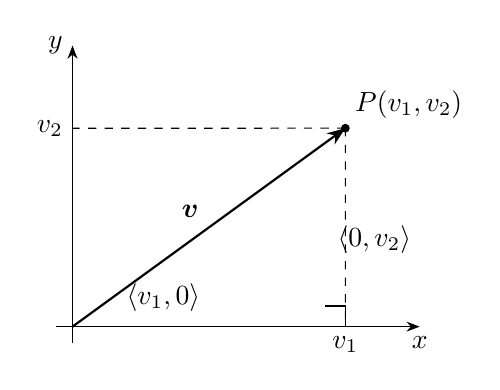
\begin{tikzpicture}[scale=1.05]
  % axes
  \draw[-{Stealth}] (-0.2,0) -- (4.2,0) node[below] {$x$};
  \draw[-{Stealth}] (0,-0.2) -- (0,3.4) node[left] {$y$};

  % point and vector
  \coordinate (O) at (0,0);
  \coordinate (P) at (3.3,2.4);
  \draw[-{Stealth},thick] (O) -- (P) node[midway,above left] {$\vect{v}$};
  \fill (P) circle (1.5pt) node[above right] {$P(v_1,v_2)$};

  % dashed projections
  \draw[dashed] (P) -- (3.3,0) node[below] {$v_1$};
  \draw[dashed] (P) -- (0,2.4) node[left] {$v_2$};

  % right angle marker
  \draw (3.3,0) -- (3.3,0.25) -- (3.05,0.25);

  % labels
  \node at (1.1,0.35) {$\langle v_1,0\rangle$};
  \node at (3.65,1.05) {$\langle 0,v_2\rangle$};
\end{tikzpicture}
\caption{A vector $\vect{v}=\langle v_1,v_2\rangle$ in $\RR^2$ and its components.}
\label{fig:vec-components}
\end{figure}

\subsubsection{Magnitude, Distance, and Unit Vectors}

\begin{definition}[Magnitude (length)]
For $\vect{v}=\langle v_1,v_2,v_3\rangle \in \RR^3$, the magnitude is
\begin{equation}\label{eq:length}
\norm{\vect{v}}=\sqrt{v_1^2+v_2^2+v_3^2}.
\end{equation}
In $\RR^2$ the same formula holds without the $v_3$ term.
\end{definition}

\begin{proposition}[Distance formula]
For points $P,Q\in \RR^n$, the distance is
\[
d(P,Q)=\norm{\overrightarrow{PQ}}.
\]
\end{proposition}

\begin{definition}[Unit vector]
If $\vect{v}\neq \vect{0}$, the unit vector in the direction of $\vect{v}$ is
\begin{equation}\label{eq:unit}
\hat{\vect{v}}=\frac{\vect{v}}{\norm{\vect{v}}}.
\end{equation}
\end{definition}

\begin{example}[Displacement, length, and direction]
Let $P=(1,-2,3)$ and $Q=(4,2,1)$. Then
\[
\overrightarrow{PQ}=\langle 4-1,\;2-(-2),\;1-3\rangle=\langle 3,4,-2\rangle.
\]
Its length is $\norm{\overrightarrow{PQ}}=\sqrt{3^2+4^2+(-2)^2}=\sqrt{29}$, and the unit direction is
\[
\widehat{\overrightarrow{PQ}}=\frac{1}{\sqrt{29}}\langle 3,4,-2\rangle.
\]
\end{example}

\subsubsection{Standard Basis and Direction Cosines}

\begin{definition}[Standard basis]
In $\RR^3$, the standard basis vectors are
\[
\vect{e}_1=\langle 1,0,0\rangle,\quad
\vect{e}_2=\langle 0,1,0\rangle,\quad
\vect{e}_3=\langle 0,0,1\rangle.
\]
Any $\vect{v}=\langle v_1,v_2,v_3\rangle$ can be written as $\vect{v}=v_1\vect{e}_1+v_2\vect{e}_2+v_3\vect{e}_3$.
\end{definition}

\begin{definition}[Direction angles and direction cosines]
Let $\vect{v}=\langle a,b,c\rangle\neq \vect{0}$ in $\RR^3$. The \emph{direction angles} $\alpha,\beta,\gamma$ are the angles between $\vect{v}$ and the positive $x$-, $y$-, $z$-axes respectively. The \emph{direction cosines} are
\begin{equation}\label{eq:dircos}
\cos\alpha=\frac{a}{\norm{\vect{v}}},\qquad
\cos\beta=\frac{b}{\norm{\vect{v}}},\qquad
\cos\gamma=\frac{c}{\norm{\vect{v}}}.
\end{equation}
They satisfy $\cos^2\alpha+\cos^2\beta+\cos^2\gamma=1$.
\end{definition}

\begin{exercise}
Let $\vect{v}=\langle -2,1,2\rangle$.
\begin{enumerate}[label=(\alph*)]
\item Compute $\norm{\vect{v}}$ and $\hat{\vect{v}}$.
\item Compute the direction cosines.
\end{enumerate}
\end{exercise}


\subsection{Lesson 1.2: Vector Operations}

\subsubsection{Addition, Subtraction, and Scalar Multiplication}

\begin{definition}[Algebraic operations]
For $\vect{u}=\langle u_1,u_2,u_3\rangle$ and $\vect{v}=\langle v_1,v_2,v_3\rangle$ in $\RR^3$ and scalar $c\in\RR$:
\[
\vect{u}+\vect{v}=\langle u_1+v_1,\;u_2+v_2,\;u_3+v_3\rangle,\qquad
\vect{u}-\vect{v}=\langle u_1-v_1,\;u_2-v_2,\;u_3-v_3\rangle,
\]
\[
c\vect{v}=\langle cv_1,\;cv_2,\;cv_3\rangle.
\]
(Identical formulas hold in $\RR^2$.)
\end{definition}

\begin{figure}[H]
\centering
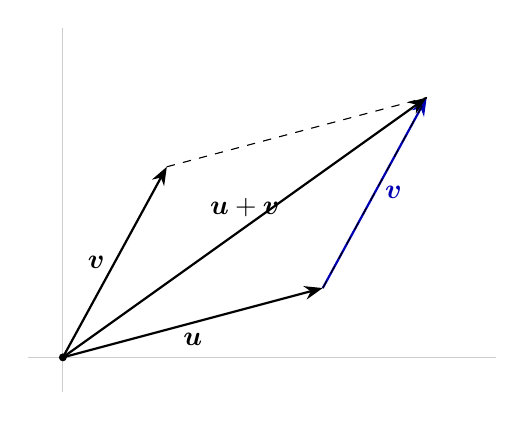
\begin{tikzpicture}[scale=1.1]
  \coordinate (O) at (0,0);
  \coordinate (U) at (3.0,0.8);
  \coordinate (V) at (1.2,2.2);
  \coordinate (S) at (4.2,3.0);

  % axes (light)
  \draw[gray!40] (-0.4,0) -- (5.0,0);
  \draw[gray!40] (0,-0.4) -- (0,3.8);

  % vectors
  \draw[-{Stealth},thick] (O) -- (U) node[midway,below] {$\vect{u}$};
  \draw[-{Stealth},thick] (O) -- (V) node[midway,left] {$\vect{v}$};

  % translated vector
  \draw[-{Stealth},thick,blue!70!black] (U) -- (S) node[midway,right] {$\vect{v}$};

  % sum
  \draw[-{Stealth},thick] (O) -- (S) node[midway,above] {$\vect{u}+\vect{v}$};

  % parallelogram edges
  \draw[dashed] (V) -- (S);
  \draw[dashed] (U) -- (S);

  \fill (O) circle (1.3pt);
\end{tikzpicture}
\caption{Vector addition via the head-to-tail rule / parallelogram rule.}
\label{fig:addition}
\end{figure}

\begin{remark}[Geometric meaning]
$\vect{u}+\vect{v}$ means: start at the tail of $\vect{u}$, walk to its head, then place $\vect{v}$ at that head and walk again. The overall displacement is the sum.
\end{remark}

\subsubsection{Linear Combinations and Span}

\begin{definition}[Linear combination]
A vector of the form $a\vect{u}+b\vect{v}$ (with scalars $a,b\in\RR$) is called a \emph{linear combination} of $\vect{u}$ and $\vect{v}$.
\end{definition}

\begin{keyidea}
Thinking in linear combinations is the bridge from geometry to computation: choose convenient vectors, then express what you need as a combination of them.
\end{keyidea}

\begin{example}[Midpoint formula as a vector statement]
Let $A,B\in\RR^n$ with position vectors $\vect{a},\vect{b}$. The midpoint $M$ of segment $AB$ has position vector
\[
\vect{m}=\frac{\vect{a}+\vect{b}}{2}.
\]
\emph{Reason:} from $A$, moving halfway toward $B$ means adding $\tfrac12(\vect{b}-\vect{a})$:
$\vect{m}=\vect{a}+\tfrac12(\vect{b}-\vect{a})=\tfrac12(\vect{a}+\vect{b})$.
\end{example}

\subsubsection{Basic Vector Identities}

\begin{proposition}[Core identities]
For vectors $\vect{u},\vect{v},\vect{w}$ and scalar $c$:
\[
\vect{u}+\vect{v}=\vect{v}+\vect{u},\quad
(\vect{u}+\vect{v})+\vect{w}=\vect{u}+(\vect{v}+\vect{w}),\quad
c(\vect{u}+\vect{v})=c\vect{u}+c\vect{v},
\]
\[
(c+d)\vect{v}=c\vect{v}+d\vect{v},\quad
c(d\vect{v})=(cd)\vect{v},\quad
1\cdot\vect{v}=\vect{v},\quad
0\cdot\vect{v}=\vect{0}.
\]
\end{proposition}

\begin{exercise}
Let $\vect{u}=\langle 1,-2,0\rangle$ and $\vect{v}=\langle 3,1,4\rangle$.
\begin{enumerate}[label=(\alph*)]
\item Compute $\vect{u}+2\vect{v}$ and $\vect{v}-\vect{u}$.
\item Find scalars $a,b$ such that $a\vect{u}+b\vect{v}=\langle 7,0,8\rangle$ (if possible).
\end{enumerate}
\end{exercise}


\subsection{Lesson 1.3: The Dot Product}

\subsubsection{Definition and Algebraic Properties}

\begin{definition}[Dot product]
For $\vect{a}=\langle a_1,\dots,a_n\rangle$ and $\vect{b}=\langle b_1,\dots,b_n\rangle$ in $\RR^n$, the \emph{dot product} is
\begin{equation}\label{eq:dot}
\vect{a}\cdot\vect{b}=\sum_{i=1}^n a_i b_i.
\end{equation}
\end{definition}

\begin{proposition}[Basic properties]
For $\vect{a},\vect{b},\vect{c}\in\RR^n$ and $k\in\RR$:
\[
\vect{a}\cdot\vect{b}=\vect{b}\cdot\vect{a},\quad
(\vect{a}+\vect{b})\cdot\vect{c}=\vect{a}\cdot\vect{c}+\vect{b}\cdot\vect{c},\quad
(k\vect{a})\cdot\vect{b}=k(\vect{a}\cdot\vect{b}).
\]
Also $\vect{a}\cdot\vect{a}\ge 0$ with equality iff $\vect{a}=\vect{0}$.
\end{proposition}

\begin{remark}[Length from dot product]
From \cref{eq:dot}, we get $\norm{\vect{a}}=\sqrt{\vect{a}\cdot\vect{a}}$, consistent with \cref{eq:length}.
\end{remark}

\subsubsection{Geometric Interpretation, Angles, and Orthogonality}

\begin{theorem}[Dot product and angle]\label{thm:dot-angle}
For nonzero vectors $\vect{a},\vect{b}\in\RR^n$, the angle $\theta\in[0,\pi]$ between them satisfies
\begin{equation}\label{eq:dot-angle}
\vect{a}\cdot\vect{b}=\norm{\vect{a}}\;\norm{\vect{b}}\cos\theta.
\end{equation}
\end{theorem}

\begin{definition}[Orthogonality]
Vectors $\vect{a}$ and $\vect{b}$ are \emph{orthogonal} (perpendicular) if $\vect{a}\cdot\vect{b}=0$.
\end{definition}

\subsubsection{Projections}

\begin{definition}[Vector projection]
For $\vect{b}\neq\vect{0}$, the projection of $\vect{a}$ onto $\vect{b}$ is
\begin{equation}\label{eq:proj}
\operatorname{proj}_{\vect{b}}(\vect{a})
=\left(\frac{\vect{a}\cdot\vect{b}}{\norm{\vect{b}}^2}\right)\vect{b}.
\end{equation}
The \emph{scalar projection} (signed length) is
$\operatorname{comp}_{\vect{b}}(\vect{a})=\dfrac{\vect{a}\cdot\vect{b}}{\norm{\vect{b}}}$.
\end{definition}

\begin{figure}[H]
\centering
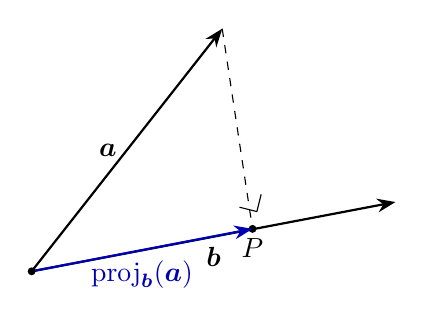
\begin{tikzpicture}[scale=1.1]
  \coordinate (O) at (0,0);
  \coordinate (B) at (4.2,0.8);
  \coordinate (A) at (2.2,2.8);

  % baseline b
  \draw[-{Stealth},thick] (O) -- (B) node[midway,below] {$\vect{b}$};

  % vector a
  \draw[-{Stealth},thick] (O) -- (A) node[midway,left] {$\vect{a}$};

  % projection point
  % compute a perpendicular drop visually by choosing a point on line OB
  \coordinate (P) at (2.55,0.49);

  \draw[dashed] (A) -- (P);
  \fill (P) circle (1.3pt) node[below] {$P$};

  % proj vector
  \draw[-{Stealth},thick,blue!70!black] (O) -- (P) node[midway,below] {$\operatorname{proj}_{\vect{b}}(\vect{a})$};

  % right angle marker at P (approx)
  \draw (P) ++(-0.15,0.25) -- ++(0.20,-0.05) -- ++(0.05,0.20);

  \fill (O) circle (1.3pt);
\end{tikzpicture}
\caption{Projection of $\vect{a}$ onto $\vect{b}$: the shadow of $\vect{a}$ along the direction of $\vect{b}$.}
\label{fig:projection}
\end{figure}

\begin{example}[Angle and projection]
Let $\vect{a}=\langle 1,2,2\rangle$ and $\vect{b}=\langle 2,1,-2\rangle$.
\[
\vect{a}\cdot\vect{b}=1\cdot 2+2\cdot 1+2\cdot(-2)=2+2-4=0,
\]
so $\vect{a}\perp\vect{b}$. Therefore the projection in \cref{eq:proj} is $\operatorname{proj}_{\vect{b}}(\vect{a})=\vect{0}$.
\end{example}

\begin{exercise}
A force $\vect{F}=\langle 10,0,0\rangle$ moves an object along displacement $\vect{d}=\langle 3,4,0\rangle$.  
Compute the work $W=\vect{F}\cdot\vect{d}$ and interpret it geometrically via \cref{thm:dot-angle}.
\end{exercise}


\subsection{Lesson 1.4: The Cross Product}

\subsubsection{Definition and Computation}

\begin{definition}[Cross product in $\RR^3$]
For $\vect{a}=\langle a_1,a_2,a_3\rangle$ and $\vect{b}=\langle b_1,b_2,b_3\rangle$ in $\RR^3$, the \emph{cross product} is
\begin{equation}\label{eq:cross}
\vect{a}\times\vect{b}
=
\left\langle
a_2b_3-a_3b_2,\;
a_3b_1-a_1b_3,\;
a_1b_2-a_2b_1
\right\rangle.
\end{equation}
\end{definition}

\begin{proposition}[Algebraic properties]
For $\vect{a},\vect{b},\vect{c}\in\RR^3$ and $k\in\RR$:
\[
\vect{a}\times\vect{b}=-(\vect{b}\times\vect{a}),\qquad
(\vect{a}+\vect{b})\times\vect{c}=\vect{a}\times\vect{c}+\vect{b}\times\vect{c},\qquad
(k\vect{a})\times\vect{b}=k(\vect{a}\times\vect{b}),
\]
and $\vect{a}\times\vect{a}=\vect{0}$.
\end{proposition}

\subsubsection{Geometry: Orientation and Area}

\begin{theorem}[Magnitude and geometric meaning]\label{thm:cross-geom}
If $\theta$ is the angle between nonzero $\vect{a},\vect{b}\in\RR^3$, then
\begin{equation}\label{eq:cross-mag}
\norm{\vect{a}\times\vect{b}}=\norm{\vect{a}}\;\norm{\vect{b}}\sin\theta.
\end{equation}
Moreover, $\vect{a}\times\vect{b}$ is perpendicular to both $\vect{a}$ and $\vect{b}$, with direction determined by the right-hand rule.
\end{theorem}

\begin{keyidea}
Dot product measures \emph{alignment} (via $\cos\theta$). Cross product measures \emph{perpendicular area} (via $\sin\theta$) and produces a \emph{normal direction}.
\end{keyidea}

\begin{figure}[H]
\centering
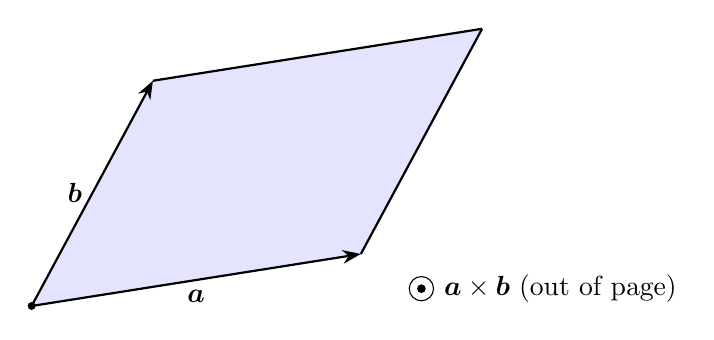
\begin{tikzpicture}[scale=1.1]
  \coordinate (O) at (0,0);
  \coordinate (A) at (3.8,0.6);
  \coordinate (B) at (1.4,2.6);
  \coordinate (C) at (5.2,3.2);

  % parallelogram fill
  \fill[blue!15,opacity=0.7] (O) -- (A) -- (C) -- (B) -- cycle;

  % edges
  \draw[-{Stealth},thick] (O) -- (A) node[midway,below] {$\vect{a}$};
  \draw[-{Stealth},thick] (O) -- (B) node[midway,left] {$\vect{b}$};
  \draw[thick] (A) -- (C);
  \draw[thick] (B) -- (C);

  % indicate normal direction (out of page) as a dot in a circle
  \draw (4.5,0.2) circle (0.14);
  \fill (4.5,0.2) circle (0.05);
  \node[right] at (4.65,0.2) {$\vect{a}\times\vect{b}$ (out of page)};

  \fill (O) circle (1.3pt);
\end{tikzpicture}
\caption{The area of the parallelogram spanned by $\vect{a}$ and $\vect{b}$ equals $\norm{\vect{a}\times\vect{b}}$.}
\label{fig:cross-area}
\end{figure}

\begin{corollary}[Areas]
The area of the parallelogram spanned by $\vect{a},\vect{b}$ is $\norm{\vect{a}\times\vect{b}}$, and the area of the triangle spanned by them is $\tfrac12\norm{\vect{a}\times\vect{b}}$.
\end{corollary}

\begin{example}[Area of a triangle from three points]
Let $A=(1,0,0)$, $B=(2,1,0)$, and $C=(0,2,1)$. Then
\[
\overrightarrow{AB}=\langle 1,1,0\rangle,\qquad
\overrightarrow{AC}=\langle -1,2,1\rangle.
\]
Compute
\[
\overrightarrow{AB}\times\overrightarrow{AC}
=
\langle 1\cdot 1-0\cdot 2,\; 0\cdot(-1)-1\cdot 1,\; 1\cdot 2-1\cdot(-1)\rangle
=
\langle 1,-1,3\rangle.
\]
So $\norm{\overrightarrow{AB}\times\overrightarrow{AC}}=\sqrt{1^2+(-1)^2+3^2}=\sqrt{11}$, and the triangle area is $\dfrac12\sqrt{11}$.
\end{example}

\begin{exercise}
Find a nonzero normal vector to the plane through $P=(1,0,2)$, $Q=(2,1,2)$, and $R=(0,2,3)$ using a cross product.
\end{exercise}


\subsection{Lesson 1.5: Lines and Planes in Space}

\subsubsection{Vector and Parametric Equations of Lines}

\begin{definition}[Line in $\RR^3$]
A line through a point with position vector $\vect{r}_0$ and direction vector $\vect{v}\neq \vect{0}$ has vector equation
\begin{equation}\label{eq:line-vector}
\vect{r}(t)=\vect{r}_0+t\vect{v},\qquad t\in\RR.
\end{equation}
If $\vect{r}=\langle x,y,z\rangle$, $\vect{r}_0=\langle x_0,y_0,z_0\rangle$, and $\vect{v}=\langle a,b,c\rangle$, then \cref{eq:line-vector} is equivalent to the parametric equations
\begin{equation}\label{eq:line-param}
x=x_0+at,\qquad y=y_0+bt,\qquad z=z_0+ct.
\end{equation}
\end{definition}

\begin{example}[Line through two points]
The line through $P=(1,2,0)$ and $Q=(4,0,3)$ has direction $\overrightarrow{PQ}=\langle 3,-2,3\rangle$, hence
\[
\vect{r}(t)=\langle 1,2,0\rangle+t\langle 3,-2,3\rangle.
\]
\end{example}

\subsubsection{Equations of Planes}

\begin{definition}[Plane (point-normal form)]
A plane through $\vect{r}_0$ with normal vector $\vect{n}\neq \vect{0}$ is the set of points $\vect{r}$ satisfying
\begin{equation}\label{eq:plane-point-normal}
\vect{n}\cdot(\vect{r}-\vect{r}_0)=0.
\end{equation}
\end{definition}

\begin{remark}[From point-normal to $ax+by+cz=d$]
If $\vect{n}=\langle a,b,c\rangle$ and $\vect{r}=\langle x,y,z\rangle$, then \cref{eq:plane-point-normal} becomes
\[
a(x-x_0)+b(y-y_0)+c(z-z_0)=0
\quad\Longleftrightarrow\quad
ax+by+cz=d,\ \ d=ax_0+by_0+cz_0.
\]
\end{remark}

\begin{figure}[H]
\centering
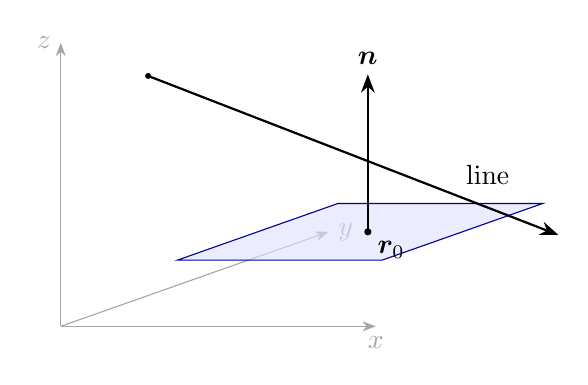
\begin{tikzpicture}[scale=1.0,
  x={(1.0cm,0.0cm)},
  y={(0.85cm,0.30cm)},
  z={(0.0cm,1.0cm)}]

  % axes
  \draw[-{Stealth},gray!70] (0,0,0) -- (4.0,0,0) node[below] {$x$};
  \draw[-{Stealth},gray!70] (0,0,0) -- (0,4.0,0) node[right] {$y$};
  \draw[-{Stealth},gray!70] (0,0,0) -- (0,0,3.6) node[left] {$z$};

  % plane as a parallelogram (z = 0.6)
  \coordinate (A) at (0.8,0.8,0.6);
  \coordinate (B) at (3.4,0.8,0.6);
  \coordinate (C) at (3.4,3.2,0.6);
  \coordinate (D) at (0.8,3.2,0.6);

  \fill[blue!12,opacity=0.6] (A) -- (B) -- (C) -- (D) -- cycle;
  \draw[blue!60!black] (A) -- (B) -- (C) -- (D) -- cycle;

  % point on plane
  \coordinate (P0) at (2.2,2.0,0.6);
  \fill (P0) circle (1.3pt) node[below right] {$\vect{r}_0$};

  % normal vector
  \coordinate (Ntip) at (2.2,2.0,2.6);
  \draw[-{Stealth},thick] (P0) -- (Ntip) node[above] {$\vect{n}$};

  % a line (direction v) passing through a point above plane
  \coordinate (L0) at (0.6,0.6,3.0);
  \coordinate (L1) at (3.6,3.2,0.2);
  \draw[-{Stealth},thick] (L0) -- (L1) node[near end,above right] {line};

  % mark L0
  \fill (L0) circle (1.1pt);

\end{tikzpicture}
\caption{A plane with normal vector $\vect{n}$ and a line in space.}
\label{fig:line-plane}
\end{figure}

\subsubsection{Distances Between Points, Lines, and Planes}

\begin{proposition}[Distance from a point to a plane]\label{prop:dist-point-plane}
For a plane $ax+by+cz=d$ and point $P=(x_0,y_0,z_0)$, the distance is
\begin{equation}\label{eq:dist-point-plane}
\operatorname{dist}(P,\Pi)=\frac{|ax_0+by_0+cz_0-d|}{\sqrt{a^2+b^2+c^2}}.
\end{equation}
\end{proposition}

\begin{remark}[Why the formula is reasonable]
The numerator is the signed ``how much the plane equation fails'' at $P$. Dividing by $\sqrt{a^2+b^2+c^2}=\norm{\langle a,b,c\rangle}$ rescales that failure into an actual geometric distance along the normal direction.
\end{remark}

\begin{proposition}[Distance from a point to a line in $\RR^3$]\label{prop:dist-point-line}
Let a line be $\vect{r}(t)=\vect{r}_0+t\vect{v}$ with $\vect{v}\neq \vect{0}$. For a point with position vector $\vect{p}$,
\begin{equation}\label{eq:dist-point-line}
\operatorname{dist}(P,\ell)=\frac{\norm{(\vect{p}-\vect{r}_0)\times\vect{v}}}{\norm{\vect{v}}}.
\end{equation}
\end{proposition}

\begin{example}[Point-to-plane distance]
Find the distance from $P=(1,2,3)$ to the plane $2x-y+2z=5$.
Using \cref{eq:dist-point-plane} with $(a,b,c,d)=(2,-1,2,5)$:
\[
\operatorname{dist}(P,\Pi)=\frac{|2(1)-1(2)+2(3)-5|}{\sqrt{2^2+(-1)^2+2^2}}
=\frac{|2-2+6-5|}{\sqrt{9}}
=\frac{1}{3}.
\]
\end{example}

\begin{example}[Plane through three points]
Find an equation for the plane through $A=(1,0,2)$, $B=(2,1,2)$, $C=(0,2,3)$.
Compute direction vectors
\[
\overrightarrow{AB}=\langle 1,1,0\rangle,\qquad
\overrightarrow{AC}=\langle -1,2,1\rangle,
\]
so a normal is
\[
\vect{n}=\overrightarrow{AB}\times\overrightarrow{AC}=\langle 1,-1,3\rangle
\]
(as in a previous computation pattern). Using point-normal form \cref{eq:plane-point-normal} with $\vect{r}_0=\langle 1,0,2\rangle$:
\[
\langle 1,-1,3\rangle\cdot\langle x-1,\ y-0,\ z-2\rangle=0
\]
\[
(x-1)-y+3(z-2)=0
\quad\Longleftrightarrow\quad
x-y+3z=7.
\]
\end{example}

\begin{exercise}
A line is given by $\vect{r}(t)=\langle 1,0,1\rangle+t\langle 2,-1,2\rangle$.
\begin{enumerate}[label=(\alph*)]
\item Determine whether the line is parallel to the plane $2x+y-2z=3$.
\item Compute the distance from $P=(0,1,0)$ to the line using \cref{eq:dist-point-line}.
\end{enumerate}
\end{exercise}

\subsubsection*{Chapter 1 Checklist}
\begin{itemize}
\item Convert between points and displacement vectors; compute lengths and unit vectors \cref{eq:length,eq:unit}.
\item Compute dot products; use them for angles and projections \cref{eq:dot-angle,eq:proj}.
\item Compute cross products; use them for normals and areas \cref{eq:cross,eq:cross-mag}.
\item Write lines and planes in vector/parametric/normal forms \cref{eq:line-vector,eq:plane-point-normal}.
\item Use projection-based distance formulas to lines/planes \cref{eq:dist-point-plane,eq:dist-point-line}.
\end{itemize}

% =========================
% End of Chapter 1
% =========================

% =========================
% Chapter 2 (no preamble)
% =========================

\section{Chapter 2: Vector-Valued Functions and Space Curves}

\begin{keyidea}
A \emph{vector-valued function} $\vect r(t)$ packages several scalar functions into one object. Geometrically, it traces a \emph{parametrized curve} in space. Once you accept “differentiate and integrate componentwise,” the calculus becomes familiar; the new content is the \emph{geometry}: tangent vectors, speed, arc length, curvature, and how acceleration splits into tangential/normal parts.
\end{keyidea}

\subsection{Lesson 2.1: Vector-Valued Functions}

\subsubsection{Definitions and Examples}

\begin{definition}[Vector-valued function]
A \emph{vector-valued function} is a function
\[
\vect r:I\subset\RR \to \RR^n,\qquad
\vect r(t)=\langle f_1(t),f_2(t),\dots,f_n(t)\rangle,
\]
where each $f_i$ is a scalar function on $I$.
When $n=2$ or $3$, $\vect r(t)$ defines a \emph{parametric curve} in the plane or in space.
\end{definition}

\begin{example}[A standard space curve: helix]
\[
\vect r(t)=\langle \cos t,\ \sin t,\ t\rangle,\qquad t\in[0,4\pi].
\]
As $t$ increases, $(\cos t,\sin t)$ runs around the unit circle while $z=t$ rises linearly, forming a helix.
\end{example}

\begin{remark}[Most intuitive interpretation]
Think of $t$ as “time.” Then $\vect r(t)$ is the position of a particle at time $t$. This viewpoint turns derivatives into velocity/acceleration automatically.
\end{remark}

\subsubsection{Limits and Continuity}

\begin{definition}[Limit of a vector-valued function]\label{def:limit-vvf}
Let $\vect r(t)=\langle f_1(t),\dots,f_n(t)\rangle$. We say
\[
\lim_{t\to a}\vect r(t)=\vect L=\langle L_1,\dots,L_n\rangle
\]
if and only if $\lim_{t\to a} f_i(t)=L_i$ for every component $i=1,\dots,n$.
\end{definition}

\begin{proposition}[Continuity]\label{prop:cont-vvf}
$\vect r$ is continuous at $t=a$ if and only if each component $f_i$ is continuous at $a$.
\end{proposition}

\begin{example}[Componentwise limit]
Let $\vect r(t)=\langle t^2,\ \sin t,\ e^t\rangle$. Then
\[
\lim_{t\to 0}\vect r(t)=\langle 0,\ 0,\ 1\rangle.
\]
\end{example}

\subsubsection{Graphs of Vector-Valued Functions (Parametric Curves)}

\begin{definition}[Parameter and trace]
The \emph{graph} of $\vect r(t)$ (often called its \emph{trace}) is the set of points in $\RR^n$:
\[
\{\vect r(t): t\in I\}.
\]
Changing the parameterization can trace the same geometric curve with different speed or orientation.
\end{definition}

\begin{figure}[H]
\centering
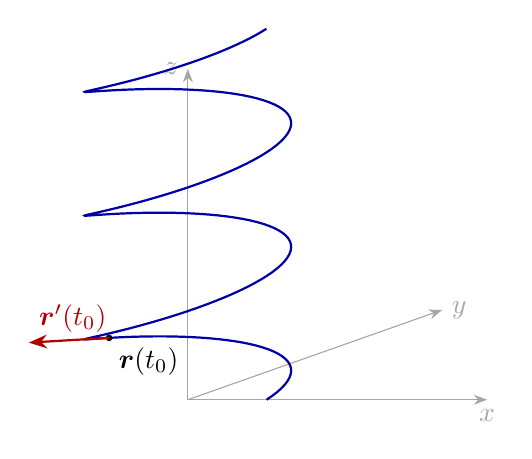
\begin{tikzpicture}[scale=1.0,
  x={(1.0cm,0.0cm)},
  y={(0.85cm,0.30cm)},
  z={(0.0cm,1.0cm)}]

  % axes
  \draw[-{Stealth},gray!70] (0,0,0) -- (3.8,0,0) node[below] {$x$};
  \draw[-{Stealth},gray!70] (0,0,0) -- (0,3.8,0) node[right] {$y$};
  \draw[-{Stealth},gray!70] (0,0,0) -- (0,0,4.2) node[left] {$z$};

  % helix: r(t) = <cos t, sin t, 0.25 t>, t in [0, 6\pi]
  \draw[thick,blue!65!black]
    plot[variable=\t,domain=0:18.8496,samples=220]
    ({cos(deg(\t))},{sin(deg(\t))},{0.25*\t});

  % mark a point at t0 = pi
  \pgfmathsetmacro{\tzero}{3.14159}
  \pgfmathsetmacro{\Px}{cos(deg(\tzero))}
  \pgfmathsetmacro{\Py}{sin(deg(\tzero))}
  \pgfmathsetmacro{\Pz}{0.25*\tzero}

  \fill (\Px,\Py,\Pz) circle (1.2pt);
  \node[below right] at (\Px,\Py,\Pz) {$\vect r(t_0)$};

  % tangent direction ~ r'(t0) = <-sin t0, cos t0, 0.25>
  \pgfmathsetmacro{\dX}{-sin(deg(\tzero))}
  \pgfmathsetmacro{\dY}{cos(deg(\tzero))}
  \pgfmathsetmacro{\dZ}{0.25}

  \draw[-{Stealth},thick,red!70!black]
    (\Px,\Py,\Pz) -- ({\Px+1.2*\dX},{\Py+1.2*\dY},{\Pz+1.2*\dZ})
    node[above right] {$\vect r'(t_0)$};

\end{tikzpicture}
\caption{A space curve (helix) traced by a vector-valued function, with a tangent (velocity) vector at $t_0$.}
\label{fig:helix}
\end{figure}

\begin{exercise}
Give two different parameterizations of the line segment from $A=(0,0,0)$ to $B=(2,1,3)$. (Hint: one can trace it in 1 second, another in 5 seconds.)
\end{exercise}


\subsection{Lesson 2.2: Derivatives of Vector-Valued Functions}

\subsubsection{Componentwise Differentiation}

\begin{definition}[Derivative]\label{def:vvf-derivative}
Let $\vect r(t)=\langle f_1(t),\dots,f_n(t)\rangle$. If each $f_i'(t)$ exists, define
\[
\vect r'(t)=\left\langle f_1'(t),f_2'(t),\dots,f_n'(t)\right\rangle.
\]
\end{definition}

\begin{proposition}[Derivative rules]
All standard rules apply componentwise: linearity, product rules for scalar multiples, and chain rule for each component.
\end{proposition}

\subsubsection{Velocity and Acceleration Vectors}

\begin{definition}[Kinematics in vector form]\label{def:kinematics}
If $\vect r(t)$ is a position vector in $\RR^3$, then
\[
\vect v(t)=\vect r'(t)\quad \text{(velocity)},\qquad
\vect a(t)=\vect r''(t)\quad \text{(acceleration)}.
\]
The \emph{speed} is the scalar $\norm{\vect v(t)}$.
\end{definition}

\begin{remark}[Plain-language meaning]
$\vect v(t)$ points in the direction of motion; its length is “how fast.” $\vect a(t)$ measures how velocity changes: it captures both speeding up/slowing down and turning.
\end{remark}

\subsubsection{Tangent Vectors and Tangent Lines}

\begin{definition}[Tangent line]\label{def:tangent-line}
If $\vect r$ is differentiable at $t=t_0$ and $\vect r'(t_0)\neq\vect 0$, the tangent line at $t_0$ is
\[
\ell:\ \vect \ell(s)=\vect r(t_0)+s\,\vect r'(t_0),\qquad s\in\RR.
\]
(Using $s$ avoids confusion with the original parameter $t$.)
\end{definition}

\begin{example}[Differentiate and form a tangent line]
Let $\vect r(t)=\langle \cos t,\ \sin t,\ t\rangle$.
Then
\[
\vect r'(t)=\langle -\sin t,\ \cos t,\ 1\rangle,\qquad
\vect r''(t)=\langle -\cos t,\ -\sin t,\ 0\rangle.
\]
At $t_0=0$,
\[
\vect r(0)=\langle 1,0,0\rangle,\qquad
\vect r'(0)=\langle 0,1,1\rangle,
\]
so the tangent line is $\vect \ell(s)=\langle 1,0,0\rangle+s\langle 0,1,1\rangle$.
\end{example}

\begin{figure}[H]
\centering
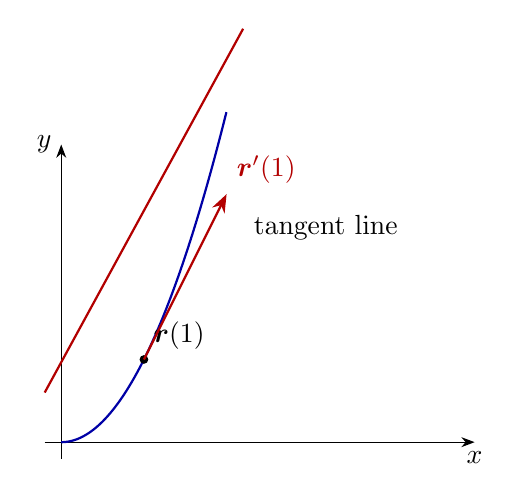
\begin{tikzpicture}[scale=1.05]
  % axes
  \draw[-{Stealth}] (-0.2,0) -- (5.0,0) node[below] {$x$};
  \draw[-{Stealth}] (0,-0.2) -- (0,3.6) node[left] {$y$};

  % curve: r(t)=<t, t^2>, t in [0,2]
  \draw[thick,blue!65!black]
    plot[variable=\t,domain=0:2,samples=140]
    ({\t},{\t*\t});

  % point at t0=1
  \coordinate (P) at (1,1);
  \fill (P) circle (1.5pt) node[above right] {$\vect r(1)$};

  % tangent line at t0=1: slope = 2
  \draw[thick,red!70!black] (-0.2,0.6) -- (2.2,5.0);

  % tangent vector r'(1)=<1,2>
  \draw[-{Stealth},thick,red!70!black] (P) -- (2.0,3.0) node[above right] {$\vect r'(1)$};

  \node at (3.2,2.6) {tangent line};
\end{tikzpicture}
\caption{Planar parametric curve $\vect r(t)=\langle t,t^2\rangle$ with tangent vector and tangent line at $t_0=1$.}
\label{fig:tangent2d}
\end{figure}

\begin{exercise}
Let $\vect r(t)=\langle e^t,\ t^2,\ \ln(1+t)\rangle$ (domain $t>-1$).
Compute $\vect r'(t)$ and the tangent line at $t_0=0$.
\end{exercise}


\subsection{Lesson 2.3: Integrals of Vector-Valued Functions}

\subsubsection{Antiderivatives}

\begin{definition}[Indefinite integral]
If $\vect r(t)=\langle f(t),g(t),h(t)\rangle$ is continuous, define
\[
\int \vect r(t)\,dt
=
\left\langle \int f(t)\,dt,\ \int g(t)\,dt,\ \int h(t)\,dt \right\rangle
=
\vect R(t)+\vect C,
\]
where $\vect R'(t)=\vect r(t)$ and $\vect C$ is a constant vector.
\end{definition}

\begin{proposition}[Fundamental Theorem (vector form)]\label{prop:ftc-vector}
If $\vect r$ is continuous on $[a,b]$ and $\vect R'(t)=\vect r(t)$, then
\[
\int_a^b \vect r(t)\,dt=\vect R(b)-\vect R(a).
\]
\end{proposition}

\subsubsection{Definite Integrals}

\begin{definition}[Definite integral]\label{def:defint-vvf}
For continuous $\vect r(t)=\langle f_1(t),\dots,f_n(t)\rangle$,
\[
\int_a^b \vect r(t)\,dt
=
\left\langle \int_a^b f_1(t)\,dt,\ \dots,\ \int_a^b f_n(t)\,dt\right\rangle.
\]
\end{definition}

\subsubsection{Applications to Motion}

\begin{proposition}[Displacement from velocity]\label{prop:disp-from-vel}
If $\vect v(t)=\vect r'(t)$, then
\[
\vect r(b)-\vect r(a)=\int_a^b \vect v(t)\,dt.
\]
\end{proposition}

\begin{remark}[Displacement vs.\ distance traveled]
\emph{Displacement} is the net change in position: $\vect r(b)-\vect r(a)$.  
\emph{Total distance traveled} is
\[
\int_a^b \norm{\vect v(t)}\,dt,
\]
which is generally larger (unless you move without reversing/turning).
\end{remark}

\begin{example}[Displacement and distance]
Let $\vect v(t)=\langle 1,\ 2t,\ 0\rangle$ for $t\in[0,2]$, and $\vect r(0)=\langle 0,0,0\rangle$.
Then
\[
\vect r(t)=\int_0^t \vect v(s)\,ds
=
\left\langle \int_0^t 1\,ds,\ \int_0^t 2s\,ds,\ 0\right\rangle
=
\langle t,\ t^2,\ 0\rangle.
\]
So displacement on $[0,2]$ is $\vect r(2)-\vect r(0)=\langle 2,4,0\rangle$.
Distance traveled is
\[
\int_0^2 \norm{\vect v(t)}\,dt=\int_0^2 \sqrt{1+(2t)^2}\,dt.
\]
(Closed form exists, but the key point is the setup: distance uses speed $\norm{\vect v}$.)
\end{example}

\begin{exercise}
Suppose $\vect a(t)=\langle 0,-g,0\rangle$ with constant $g>0$, and $\vect v(0)=\langle v_0,0,0\rangle$, $\vect r(0)=\langle 0,0,0\rangle$.
Find $\vect v(t)$ and $\vect r(t)$.
\end{exercise}


\subsection{Lesson 2.4: Arc Length and Curvature}

\subsubsection{Arc Length of Space Curves}

\begin{theorem}[Arc length formula]\label{thm:arc-length}
If $\vect r:[a,b]\to\RR^3$ is continuously differentiable, then the arc length of its trace is
\begin{equation}\label{eq:arc-length}
L=\int_a^b \norm{\vect r'(t)}\,dt.
\end{equation}
\end{theorem}

\begin{remark}[Intuition in one sentence]
Over a tiny time step $\Delta t$, you move about $\norm{\vect r'(t)}\,\Delta t$; summing these and taking a limit yields \cref{eq:arc-length}.
\end{remark}

\begin{example}[Arc length of a helix segment]
For $\vect r(t)=\langle \cos t,\ \sin t,\ t\rangle$ on $[0,2\pi]$,
\[
\vect r'(t)=\langle -\sin t,\ \cos t,\ 1\rangle,\qquad
\norm{\vect r'(t)}=\sqrt{\sin^2 t+\cos^2 t+1}=\sqrt{2}.
\]
Thus $L=\int_0^{2\pi}\sqrt{2}\,dt=2\pi\sqrt{2}$.
\end{example}

\subsubsection{Unit Tangent and Normal Vectors}

\begin{definition}[Unit tangent]\label{def:unit-tangent}
If $\vect r'(t)\neq\vect 0$, the unit tangent vector is
\begin{equation}\label{eq:unit-tangent}
\vect T(t)=\frac{\vect r'(t)}{\norm{\vect r'(t)}}.
\end{equation}
\end{definition}

\begin{definition}[Principal normal]
If $\vect T'(t)\neq\vect 0$, define the principal unit normal vector by
\[
\vect N(t)=\frac{\vect T'(t)}{\norm{\vect T'(t)}}.
\]
In $\RR^3$, one also defines the binormal $\vect B(t)=\vect T(t)\times \vect N(t)$.
\end{definition}

\subsubsection{Curvature of a Curve}

\begin{definition}[Curvature]\label{def:curvature}
Let $s$ be arc length (so $ds/dt=\norm{\vect r'(t)}$). The curvature is
\[
\kappa=\norm{\frac{d\vect T}{ds}}.
\]
Equivalently (as a function of $t$),
\begin{equation}\label{eq:curvature-t}
\kappa(t)=\frac{\norm{\vect T'(t)}}{\norm{\vect r'(t)}}.
\end{equation}
\end{definition}

\begin{theorem}[Cross-product curvature formula]\label{thm:curvature-cross}
If $\vect r$ is twice differentiable and $\vect r'(t)\neq \vect 0$, then
\begin{equation}\label{eq:curvature-cross}
\kappa(t)=\frac{\norm{\vect r'(t)\times \vect r''(t)}}{\norm{\vect r'(t)}^{3}}.
\end{equation}
\end{theorem}

\begin{example}[Curvature of $\langle \cos t,\sin t,t\rangle$ is constant]
For $\vect r(t)=\langle \cos t,\ \sin t,\ t\rangle$:
\[
\vect r'(t)=\langle -\sin t,\ \cos t,\ 1\rangle,\quad
\vect r''(t)=\langle -\cos t,\ -\sin t,\ 0\rangle.
\]
Compute
\[
\vect r'(t)\times \vect r''(t)
=
\left\langle
1\cdot(-\sin t)-1\cdot(-\sin t)?,\ \dots
\right\rangle
\]
Rather than expand blindly, do it carefully:
\begin{align*}
\vect r'(t)\times \vect r''(t) &=
\begin{vmatrix}
\vect i & \vect j & \vect k\\
-\sin t & \cos t & 1\\
-\cos t & -\sin t & 0
\end{vmatrix} \\
&= \bigl\langle
\cos t\cdot 0-1\cdot(-\sin t), \\
&\quad\quad -\bigl((-\sin t)\cdot 0-1\cdot(-\cos t)\bigr), \\
&\quad\quad (-\sin t)(-\sin t)-(\cos t)(-\cos t)
\bigr\rangle
\end{align*}
\[
=\langle \sin t,\ -\cos t,\ 1\rangle.
\]
Hence $\norm{\vect r'(t)\times \vect r''(t)}=\sqrt{\sin^2 t+\cos^2 t+1}=\sqrt{2}$ and
$\norm{\vect r'(t)}=\sqrt{2}$, so by \cref{eq:curvature-cross},
\[
\kappa(t)=\frac{\sqrt{2}}{(\sqrt{2})^3}=\frac{1}{2}.
\]
\end{example}

\begin{exercise}
For the circle $\vect r(t)=\langle a\cos t,\ a\sin t,\ 0\rangle$ ($a>0$), compute $\kappa(t)$ and interpret the result geometrically.
\end{exercise}


\subsection{Lesson 2.5: Motion in Space}

\subsubsection{Kinematics in Three Dimensions}

\begin{notation}
We will write $\vect v=\vect r'$ and $\vect a=\vect r''$ as in \cref{def:kinematics}, and speed $v=\norm{\vect v}$ (note: $v$ is a scalar here).
\end{notation}

\begin{proposition}[Decomposition of acceleration]\label{prop:acc-decomp}
Assume $\vect r'(t)\neq \vect 0$. Then acceleration splits into tangential and normal parts:
\begin{equation}\label{eq:acc-decomp}
\vect a = a_T\,\vect T + a_N\,\vect N,
\end{equation}
where
\begin{equation}\label{eq:aT}
a_T=\frac{dv}{dt}=\frac{\vect v\cdot \vect a}{\norm{\vect v}},
\qquad
a_N=\kappa v^2=\frac{\norm{\vect v\times \vect a}}{\norm{\vect v}}.
\end{equation}
\end{proposition}

\begin{remark}[What this means in plain terms]
$a_T$ measures \emph{speeding up or slowing down}.  
$a_N$ measures \emph{turning}: even if speed is constant ($a_T=0$), you can still have acceleration if the direction changes.
\end{remark}

\begin{example}[Projectile motion (in a plane, written vectorially)]
Let $g>0$ and
\[
\vect r(t)=\langle v_0\cos\theta\; t,\ v_0\sin\theta\; t-\tfrac12 g t^2,\ 0\rangle.
\]
Then
\[
\vect v(t)=\langle v_0\cos\theta,\ v_0\sin\theta-gt,\ 0\rangle,\qquad
\vect a(t)=\langle 0,\ -g,\ 0\rangle.
\]
Acceleration is constant and downward, independent of the current velocity.
\end{example}

\begin{example}[Uniform circular motion and normal acceleration]
If $\vect r(t)=\langle a\cos(\omega t),\ a\sin(\omega t),\ 0\rangle$, then
\[
\vect v(t)=\langle -a\omega\sin(\omega t),\ a\omega\cos(\omega t),\ 0\rangle,\quad
v=\norm{\vect v}=a\omega \ \text{(constant)}.
\]
Thus $a_T=dv/dt=0$. Nevertheless,
\[
\vect a(t)=\langle -a\omega^2\cos(\omega t),\ -a\omega^2\sin(\omega t),\ 0\rangle,
\]
which points toward the center and has magnitude $a\omega^2=\dfrac{v^2}{a}$, matching $a_N=\kappa v^2$ with $\kappa=1/a$.
\end{example}

\begin{exercise}
A particle moves along $\vect r(t)=\langle t,\ \cos t,\ \sin t\rangle$ for $t\ge 0$.
\begin{enumerate}[label=(\alph*)]
\item Compute $\vect v(t)$, $\vect a(t)$, and the speed $v(t)$.
\item Determine whether the speed is constant.
\item Compute $\kappa(t)$ using \cref{eq:curvature-cross}.
\end{enumerate}
\end{exercise}

\subsubsection*{Chapter 2 Checklist}
\begin{itemize}
\item Treat limits/continuity/derivatives/integrals \emph{componentwise} (Definitions \cref{def:limit-vvf,def:vvf-derivative,def:defint-vvf}).
\item Interpret $\vect r',\vect r''$ as velocity and acceleration; speed is $\norm{\vect r'}$.
\item Build tangent lines from $\vect r(t_0)$ and $\vect r'(t_0)$ (\cref{def:tangent-line}).
\item Compute arc length via $L=\int \norm{\vect r'}\,dt$ (\cref{thm:arc-length}).
\item Compute curvature via $\kappa=\norm{\vect r'\times \vect r''}/\norm{\vect r'}^3$ (\cref{thm:curvature-cross}).
\item Decompose acceleration into tangential/normal components (\cref{prop:acc-decomp}).
\end{itemize}

% =========================
% End of Chapter 2
% =========================

% =========================
% Chapter 3 (no preamble)
% =========================

\section{Chapter 3: Functions of Several Variables}

\begin{keyidea}
A single-variable function $y=f(x)$ lives on a line and draws a curve.  
A multivariable function $z=f(x,y)$ lives on a \emph{region in the plane} and draws a \emph{surface} in space.  
Because surfaces are hard to “see” directly, we use \emph{level sets} (contours) and \emph{slices} (traces) to understand them, and we use \emph{partial derivatives} to measure how the output changes when we move in chosen directions.
\end{keyidea}

% -------------------------------------------------
\subsection{Lesson 3.1: Functions of Two and Three Variables}

\subsubsection{Definitions and Examples}

\begin{definition}[Functions of several variables]
A function of two variables is a map
\[
f:D\subset \RR^2 \to \RR,\qquad (x,y)\mapsto f(x,y),
\]
where $D$ is the \emph{domain}. A function of three variables is
\[
f:D\subset \RR^3 \to \RR,\qquad (x,y,z)\mapsto f(x,y,z).
\]
The \emph{range} is $\{f(\vect x): \vect x\in D\}$.
\end{definition}

\begin{example}[Domains]
\begin{enumerate}[label=(\alph*)]
\item $f(x,y)=\sqrt{1-x^2-y^2}$ has domain $D=\{(x,y):x^2+y^2\le 1\}$ (a closed disk).
\item $g(x,y)=\dfrac{1}{x^2+y^2}$ has domain $\RR^2\setminus\{(0,0)\}$.
\item $h(x,y,z)=\ln(z-x^2-y^2)$ has domain $\{(x,y,z): z>x^2+y^2\}$.
\end{enumerate}
\end{example}

\begin{remark}[A practical rule]
Domains are determined by where the formula makes sense: no division by $0$, even roots require nonnegative input, logarithms require positive input, etc.
\end{remark}

\subsubsection{Graphs and Level Sets}

\begin{definition}[Graph of $z=f(x,y)$]
If $f:D\subset\RR^2\to\RR$, the \emph{graph} of $f$ is the set
\[
\{(x,y,z)\in\RR^3: (x,y)\in D,\ z=f(x,y)\}.
\]
\end{definition}

\begin{definition}[Level curves and level surfaces]
For $f(x,y)$, the \emph{level curve} at height $c$ is
\[
f(x,y)=c.
\]
For $F(x,y,z)$, the \emph{level surface} at level $c$ is
\[
F(x,y,z)=c.
\]
\end{definition}

\begin{example}[A classic: paraboloid and its contours]
Let $f(x,y)=x^2+y^2$.  
\begin{itemize}
\item The graph is the paraboloid $z=x^2+y^2$.
\item The level curves $x^2+y^2=c$ (for $c\ge 0$) are circles of radius $\sqrt{c}$ in the $xy$-plane.
\end{itemize}
\end{example}

\begin{figure}[H]
\centering
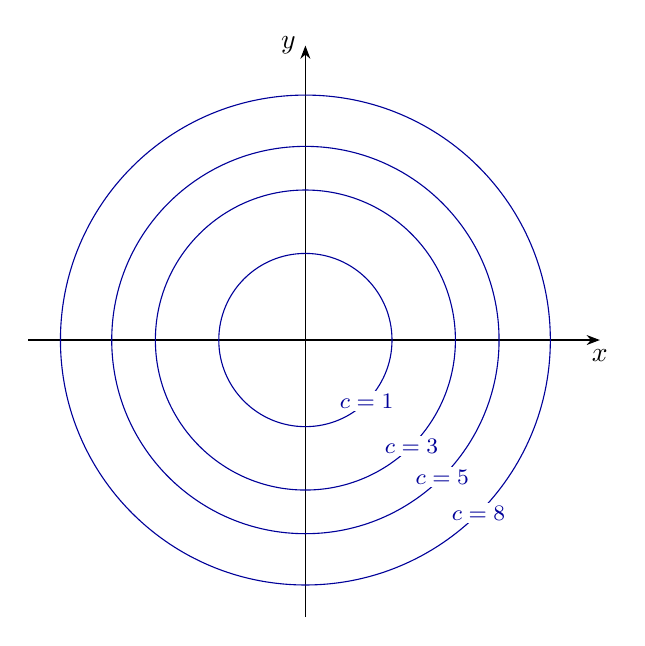
\begin{tikzpicture}[scale=1.1]
  % axes
  \draw[-{Stealth}] (-3.2,0) -- (3.4,0) node[below] {$x$};
  \draw[-{Stealth}] (0,-3.2) -- (0,3.4) node[left] {$y$};

% level curves for x^2+y^2=c
  \foreach \r/\lab in {1/1,1.732/3,2.236/5,2.828/8} {
    \draw[blue!60!black] (0,0) circle (\r);
    \node[blue!60!black, fill=white, inner sep=1pt, font=\footnotesize] at (-45:\r) {$c=\lab$};
  }
\end{tikzpicture}
\caption{Level curves (contour lines) for $f(x,y)=x^2+y^2$.}
\label{fig:levelcurves}
\end{figure}

\subsubsection{Domains and Ranges (Geometric View)}

\begin{example}[Range from geometry]
For $f(x,y)=\sqrt{1-x^2-y^2}$ with domain $x^2+y^2\le 1$, we have $0\le 1-x^2-y^2\le 1$, so
\[
0\le f(x,y)\le 1.
\]
Geometrically, $z=\sqrt{1-x^2-y^2}$ is the upper hemisphere of the unit sphere, so heights run from $0$ to $1$.
\end{example}

\begin{exercise}
Describe the domain of $f(x,y)=\dfrac{\sqrt{4-x^2}}{y-1}$ and sketch it in the $xy$-plane.
\end{exercise}

% -------------------------------------------------
\subsection{Lesson 3.2: Limits and Continuity}

\subsubsection{Limits of Multivariable Functions}

\begin{definition}[Limit in $\RR^2$]\label{def:limitR2}
Let $f:D\subset\RR^2\to\RR$ and let $(a,b)$ be a limit point of $D$. We say
\[
\lim_{(x,y)\to(a,b)} f(x,y)=L
\]
if for every $\varepsilon>0$ there exists $\delta>0$ such that whenever $(x,y)\in D$ and
\[
0<\sqrt{(x-a)^2+(y-b)^2}<\delta,
\]
we have $|f(x,y)-L|<\varepsilon$.
\end{definition}

\begin{remark}[What changed from Calc I]
In one variable, approaching $a$ means coming from the left/right on a line.  
In two variables, $(x,y)\to(a,b)$ means approaching from \emph{infinitely many paths} in the plane. This is why limits are harder: you must control \emph{all} approaches.
\end{remark}

\subsubsection{When a Limit Does Not Exist}

\begin{proposition}[Path test (useful sufficient test for nonexistence)]\label{prop:path-test}
If there exist two paths $\gamma_1,\gamma_2$ approaching $(a,b)$ such that
\[
\lim_{(x,y)\to(a,b)\ \text{along }\gamma_1} f(x,y)\neq
\lim_{(x,y)\to(a,b)\ \text{along }\gamma_2} f(x,y),
\]
then $\lim_{(x,y)\to(a,b)} f(x,y)$ does not exist.
\end{proposition}

\begin{example}[Different paths, different limits]
Define
\[
f(x,y)=
\begin{cases}
\dfrac{x^2-y^2}{x^2+y^2}, & (x,y)\neq(0,0),\\[6pt]
0, & (x,y)=(0,0).
\end{cases}
\]
Along the $x$-axis ($y=0$), for $x\neq 0$,
\[
f(x,0)=\frac{x^2}{x^2}=1 \quad\Longrightarrow\quad \lim_{x\to 0} f(x,0)=1.
\]
Along the $y$-axis ($x=0$), for $y\neq 0$,
\[
f(0,y)=\frac{-y^2}{y^2}=-1 \quad\Longrightarrow\quad \lim_{y\to 0} f(0,y)=-1.
\]
The two path limits disagree, so the limit at $(0,0)$ does not exist by \cref{prop:path-test}.
\end{example}

\begin{figure}[H]
\centering
\begin{tikzpicture}[scale=1.05]
  \draw[-{Stealth}] (-3.2,0) -- (3.2,0) node[below] {$x$};
  \draw[-{Stealth}] (0,-3.2) -- (0,3.2) node[left] {$y$};

  % two paths
  % 修改1: node[below right] 改为 node[above]，避开下方的 x
  \draw[thick,blue!65!black] (-3,0) -- (3,0) node[above] at (3,0) {$y=0$};
  
  % 修改2: node[above left] 改为 node[right]，避开左侧的 y
  \draw[thick,red!70!black] (0,-3) -- (0,3) node[right] at (0,3) {$x=0$};

  % origin
  \fill (0,0) circle (1.5pt);
  \node[below left] at (0,0) {$(0,0)$};

  \node at (0,-3.8) {Two different paths to $(0,0)$ can force different values.};
\end{tikzpicture}
\caption{Approaching $(0,0)$ along different paths is a standard way to test nonexistence of a limit.}
\label{fig:paths}
\end{figure}

\subsubsection{Continuity and Properties}

\begin{definition}[Continuity at a point]\label{def:cont-multi}
A function $f:D\subset\RR^2\to\RR$ is \emph{continuous} at $(a,b)\in D$ if
\[
\lim_{(x,y)\to(a,b)} f(x,y)=f(a,b).
\]
\end{definition}

\begin{proposition}[Algebra of continuity]
If $f$ and $g$ are continuous at $(a,b)$, then $f+g$, $f-g$, $fg$, and (where defined) $f/g$ are continuous at $(a,b)$. Compositions of continuous functions are continuous.
\end{proposition}

\begin{remark}[A reliable shortcut]
Polynomials in $(x,y)$ are continuous everywhere. Rational functions are continuous wherever the denominator is nonzero. Functions built from continuous pieces (roots, trig, exp/log) are continuous where their inputs are valid.
\end{remark}

\begin{exercise}
Determine whether $f(x,y)=\dfrac{xy}{x^2+y^2}$ (with $f(0,0)=0$) is continuous at $(0,0)$.  
(Hint: try the path $y=mx$.)
\end{exercise}

% -------------------------------------------------
\subsection{Lesson 3.3: Partial Derivatives}

\subsubsection{Definition of Partial Derivatives}

\begin{definition}[First-order partial derivatives]\label{def:partials}
Let $f(x,y)$ be defined near $(a,b)$. The partial derivatives at $(a,b)$ are
\[
f_x(a,b)=\lim_{h\to 0}\frac{f(a+h,b)-f(a,b)}{h},
\qquad
f_y(a,b)=\lim_{h\to 0}\frac{f(a,b+h)-f(a,b)}{h},
\]
if the limits exist.
\end{definition}

\begin{remark}[Plain-language interpretation]
$f_x(a,b)$ measures how $f$ changes when you move in the $x$-direction \emph{while freezing $y=b$}.  
$f_y(a,b)$ does the same in the $y$-direction \emph{while freezing $x=a$}.  
So partial derivatives are “single-variable derivatives of slices.”
\end{remark}

\subsubsection{Higher-Order Partial Derivatives}

\begin{definition}[Second-order partial derivatives]\label{def:secondpartials}
If $f_x$ and $f_y$ exist near $(a,b)$, we can differentiate again:
\[
f_{xx}=\frac{\partial}{\partial x}(f_x),\quad
f_{yy}=\frac{\partial}{\partial y}(f_y),\quad
f_{xy}=\frac{\partial}{\partial y}(f_x),\quad
f_{yx}=\frac{\partial}{\partial x}(f_y).
\]
\end{definition}

\subsubsection{Clairaut's Theorem (Equality of Mixed Partials)}

\begin{theorem}[Clairaut / Schwarz]\label{thm:clairaut}
If $f_{xy}$ and $f_{yx}$ are continuous on an open neighborhood of $(a,b)$, then
\[
f_{xy}(a,b)=f_{yx}(a,b).
\]
\end{theorem}

\begin{example}[Computing mixed partials]
Let $f(x,y)=x^2y^3+\sin(xy)$. Then
\[
f_x=2xy^3+y\cos(xy),\qquad
f_y=3x^2y^2+x\cos(xy).
\]
Differentiate again:
\[
f_{xy}=\frac{\partial}{\partial y}\left(2xy^3+y\cos(xy)\right)
=6xy^2+\cos(xy)-xy\sin(xy),
\]
\[
f_{yx}=\frac{\partial}{\partial x}\left(3x^2y^2+x\cos(xy)\right)
=6xy^2+\cos(xy)-xy\sin(xy).
\]
So $f_{xy}=f_{yx}$ (as predicted by \cref{thm:clairaut} since the formula is smooth everywhere).
\end{example}

\begin{figure}[H]
\centering
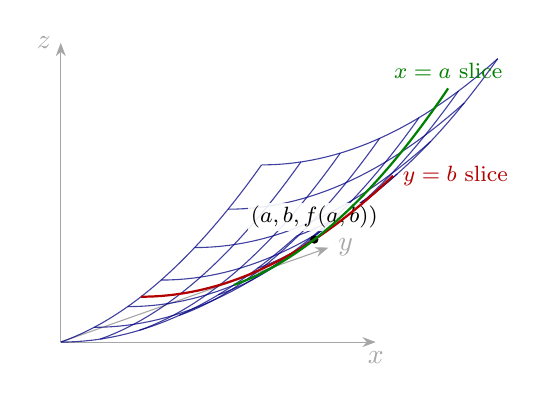
\begin{tikzpicture}[scale=1.0,
  x={(1.0cm,0.0cm)},
  y={(0.85cm,0.30cm)},
  z={(0.0cm,1.0cm)}]

  % --- 1. 定义变量 (避免使用 \b, 改用 \yb) ---
  \def\xa{2.2}
  \def\yb{1.2}

  % axes (坐标轴)
  \draw[-{Stealth},gray!70] (0,0,0) -- (4.0,0,0) node[below] {$x$};
  \draw[-{Stealth},gray!70] (0,0,0) -- (0,4.0,0) node[right] {$y$};
  \draw[-{Stealth},gray!70] (0,0,0) -- (0,0,3.8) node[left] {$z$};

  % --- 2. 绘制曲面网格 ---
  % x-direction lines
  \foreach \u in {0,0.5,...,3} {
    \draw[blue!50!black,opacity=0.75]
      plot[variable=\v,domain=0:3,samples=30]
      ({\u},{\v},{0.15*(\u*\u+\v*\v)});
  }
  % y-direction lines
  \foreach \v in {0,0.5,...,3} {
    \draw[blue!50!black,opacity=0.75]
      plot[variable=\u,domain=0:3,samples=30]
      ({\u},{\v},{0.15*(\u*\u+\v*\v)});
  }

  % --- 3. 绘制点 (a, b) ---
  % 提前计算 z 坐标，避免在 coordinate 中出错
  \pgfmathsetmacro{\zpt}{0.15*(\xa*\xa+\yb*\yb)}
  \coordinate (P) at (\xa,\yb,\zpt);
  
  \fill (P) circle (1.5pt);
  % 使用 anchor=south 稍微把文字往上提，防止盖住点
  \node[above=3pt, fill=white, inner sep=1pt, opacity=0.9, text opacity=1] at (P) {\footnotesize $(a,b,f(a,b))$};

  % --- 4. 绘制切片曲线 (Trace Lines) 并添加标签 ---

  % [红色] y=b 切片 (固定 y=\yb, 变动 x)
  \draw[thick,red!70!black]
    plot[variable=\u,domain=0:3.2,samples=40] % 稍微画长一点到 3.2 以便放置标签
    ({\u},{\yb},{0.15*(\u*\u+\yb*\yb)});
  
  % 计算红色标签的位置 (在 x=3.2 处)
  \pgfmathsetmacro{\zRedLabel}{0.15*(3.2*3.2+\yb*\yb)}
  \node[red!70!black, right, font=\footnotesize] 
    at (3.2, \yb, \zRedLabel) {$y=b$ slice};

  % [绿色] x=a 切片 (固定 x=\xa, 变动 y)
  \draw[thick,green!50!black]
    plot[variable=\v,domain=0:3.2,samples=40]
    ({\xa},{\v},{0.15*(\xa*\xa+\v*\v)});

  % 计算绿色标签的位置 (在 y=3.2 处)
  \pgfmathsetmacro{\zGreenLabel}{0.15*(\xa*\xa+3.2*3.2)}
  \node[green!50!black, above, font=\footnotesize] 
    at (\xa, 3.2, \zGreenLabel) {$x=a$ slice};

\end{tikzpicture}
\caption{Partial derivatives come from slopes of slice curves: fix $y=b$ (red) for $f_x$, fix $x=a$ (green) for $f_y$.}
\label{fig:slices}
\end{figure}

\begin{exercise}
Let $f(x,y)=\dfrac{x^2y}{1+y^2}$.
\begin{enumerate}[label=(\alph*)]
\item Compute $f_x$ and $f_y$.
\item Compute $f_{xy}$ and $f_{yx}$ and verify they agree.
\end{enumerate}
\end{exercise}

% -------------------------------------------------
\subsection{Lesson 3.4: Differentiability and the Gradient}

\subsubsection{Differentiability}

\begin{definition}[Differentiability in $\RR^2$]\label{def:differentiable}
Let $f$ be defined near $(a,b)$. We say $f$ is \emph{differentiable} at $(a,b)$ if there exists a linear map
\[
L(h,k)=Ah+Bk
\]
such that
\begin{equation}\label{eq:diff-def}
f(a+h,b+k)=f(a,b)+L(h,k)+o\!\left(\sqrt{h^2+k^2}\right)
\quad\text{as }(h,k)\to(0,0).
\end{equation}
\end{definition}

\begin{remark}[Why this matters]
Differentiability means: near $(a,b)$, the surface is well-approximated by a plane.  
Continuity alone says “no jumps,” but differentiability says “has a reliable linear approximation.”
\end{remark}

\begin{theorem}[Sufficient condition for differentiability]\label{thm:cont-partials}
If $f_x$ and $f_y$ exist in a neighborhood of $(a,b)$ and are continuous at $(a,b)$, then $f$ is differentiable at $(a,b)$.
\end{theorem}

\begin{proposition}[Differentiability implies continuity]
If $f$ is differentiable at $(a,b)$, then $f$ is continuous at $(a,b)$.
\end{proposition}

\subsubsection{The Gradient Vector}

\begin{definition}[Gradient]\label{def:gradient}
If $f:\RR^2\to\RR$ has partial derivatives, its gradient is
\[
\nabla f(x,y)=\left\langle f_x(x,y),\, f_y(x,y)\right\rangle.
\]
More generally for $f:\RR^n\to\RR$,
\[
\nabla f=\left\langle \frac{\partial f}{\partial x_1},\dots,\frac{\partial f}{\partial x_n}\right\rangle.
\]
\end{definition}

\begin{remark}[What the gradient “is”]
$\nabla f(a,b)$ points in the direction where $f$ increases fastest, and its magnitude is that maximum rate of increase (made precise below).
\end{remark}

\subsubsection{Directional Derivatives}

\begin{definition}[Directional derivative]\label{def:dirder}
Let $\vect u=\langle u_1,u_2\rangle$ be a unit vector. The directional derivative of $f$ at $(a,b)$ in direction $\vect u$ is
\[
D_{\vect u}f(a,b)=\lim_{h\to 0}\frac{f(a+hu_1,b+hu_2)-f(a,b)}{h},
\]
if the limit exists.
\end{definition}

\begin{theorem}[Directional derivative via gradient]\label{thm:dirder-grad}
If $f$ is differentiable at $(a,b)$, then for every unit vector $\vect u$,
\begin{equation}\label{eq:dirder-grad}
D_{\vect u}f(a,b)=\nabla f(a,b)\cdot \vect u.
\end{equation}
\end{theorem}

\begin{corollary}[Maximal increase]\label{cor:max-increase}
If $f$ is differentiable at $(a,b)$ and $\vect u$ is unit, then
\[
-\norm{\nabla f(a,b)} \le D_{\vect u}f(a,b)\le \norm{\nabla f(a,b)},
\]
with maximum $\norm{\nabla f(a,b)}$ achieved when $\vect u$ points in the direction of $\nabla f(a,b)$.
\end{corollary}

\begin{proof}
By \cref{eq:dirder-grad} and Cauchy--Schwarz,
\[
D_{\vect u}f(a,b)=\nabla f(a,b)\cdot \vect u \le \norm{\nabla f(a,b)}\,\norm{\vect u}
=\norm{\nabla f(a,b)}.
\]
Similarly, the minimum is $-\norm{\nabla f(a,b)}$. Equality occurs exactly when $\vect u$ is parallel (or antiparallel) to $\nabla f(a,b)$.
\end{proof}

\begin{figure}[H]
\centering
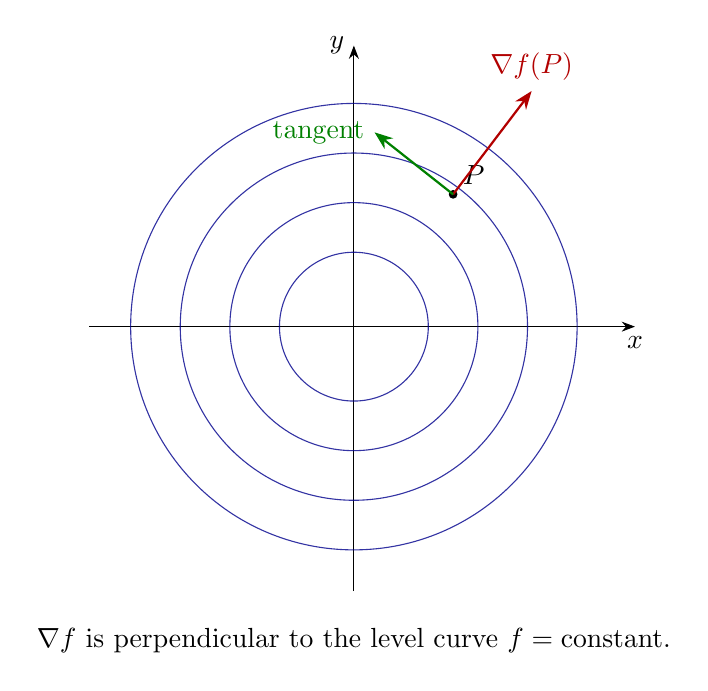
\begin{tikzpicture}[scale=1.05]
  % axes
  \draw[-{Stealth}] (-3.2,0) -- (3.4,0) node[below] {$x$};
  \draw[-{Stealth}] (0,-3.2) -- (0,3.4) node[left] {$y$};

  % contours: x^2+y^2=c
  \foreach \r in {0.9,1.5,2.1,2.7} {
    \draw[blue!55!black,opacity=0.8] (0,0) circle (\r);
  }

  % point P
  \coordinate (P) at (1.2,1.6);
  \fill (P) circle (1.5pt);
  \node[above right] at (P) {$P$};

  % gradient direction for f=x^2+y^2 is <2x,2y> at P
  % draw a normalized-ish arrow
  \draw[-{Stealth},thick,red!70!black] (P) -- (2.15,2.85) node[above] {$\nabla f(P)$};

  % a tangent direction to level curve at P (perpendicular to gradient)
  \draw[-{Stealth},thick,green!50!black] (P) -- (0.25,2.35) node[left] {tangent};

  \node at (0,-3.8) {$\nabla f$ is perpendicular to the level curve $f=\text{constant}$.};
\end{tikzpicture}
\caption{For $f(x,y)=x^2+y^2$, the gradient points radially outward and is perpendicular to the contour through $P$.}
\label{fig:grad-perp}
\end{figure}

\begin{example}[Directional derivative computation]
Let $f(x,y)=x^2y$ and $P=(1,2)$. Then
\[
\nabla f(x,y)=\langle 2xy,\ x^2\rangle
\quad\Longrightarrow\quad
\nabla f(1,2)=\langle 4,\ 1\rangle.
\]
Take the unit direction $\vect u=\frac{1}{5}\langle 3,4\rangle$. By \cref{eq:dirder-grad},
\[
D_{\vect u}f(1,2)=\langle 4,1\rangle\cdot \frac{1}{5}\langle 3,4\rangle
=\frac{1}{5}(12+4)=\frac{16}{5}.
\]
\end{example}

\begin{exercise}
Let $f(x,y)=\ln(x^2+y^2)$ (domain $(x,y)\neq(0,0)$).
\begin{enumerate}[label=(\alph*)]
\item Compute $\nabla f(x,y)$.
\item Find the directional derivative at $(1,1)$ in the direction toward $(2,0)$.
\end{enumerate}
\end{exercise}

% -------------------------------------------------
\subsection{Lesson 3.5: The Chain Rule}

\subsubsection{Chain Rule for One Parameter}

\begin{theorem}[Chain rule: $t\mapsto (x(t),y(t))$]\label{thm:chain-1}
Let $z=f(x,y)$ where $f$ has partial derivatives, and let $x=x(t)$, $y=y(t)$ be differentiable. Define
\[
z(t)=f(x(t),y(t)).
\]
Then
\begin{equation}\label{eq:chain-1}
\frac{dz}{dt}=f_x(x(t),y(t))\frac{dx}{dt}+f_y(x(t),y(t))\frac{dy}{dt}.
\end{equation}
\end{theorem}

\begin{remark}[Interpretation]
$\dfrac{dz}{dt}$ is the rate of change of $f$ along the path $(x(t),y(t))$.  
It is a weighted sum of “how sensitive $f$ is to $x$” and “how sensitive $f$ is to $y$,” weighted by how fast $x$ and $y$ are changing.
\end{remark}

\begin{example}[Compute $dz/dt$]
Let $f(x,y)=x^2+y^2$, $x(t)=e^t$, $y(t)=\sin t$. Then $z(t)=e^{2t}+\sin^2 t$ and
\[
\frac{dz}{dt}=2e^{2t}+2\sin t\cos t.
\]
Using \cref{eq:chain-1} as a check: $f_x=2x$, $f_y=2y$, so
\[
\frac{dz}{dt}=2x\frac{dx}{dt}+2y\frac{dy}{dt}
=2(e^t)(e^t)+2(\sin t)(\cos t)=2e^{2t}+2\sin t\cos t,
\]
consistent.
\end{example}

\subsubsection{Chain Rule for Two Parameters}

\begin{theorem}[Chain rule: $(s,t)\mapsto (x(s,t),y(s,t))$]\label{thm:chain-2}
Let $z=f(x,y)$ with $f_x,f_y$ defined, and let $x=x(s,t)$ and $y=y(s,t)$ be differentiable. Then
\begin{equation}\label{eq:chain-2}
\frac{\partial z}{\partial s}=f_x\,\frac{\partial x}{\partial s}+f_y\,\frac{\partial y}{\partial s},
\qquad
\frac{\partial z}{\partial t}=f_x\,\frac{\partial x}{\partial t}+f_y\,\frac{\partial y}{\partial t},
\end{equation}
where $f_x,f_y$ are evaluated at $(x(s,t),y(s,t))$.
\end{theorem}

\subsubsection{Implicit Differentiation}

\begin{theorem}[Implicit differentiation in $\RR^3$]\label{thm:implicit}
Let $F(x,y,z)=0$ define $z=z(x,y)$ near a point where $F_z\neq 0$ and $F$ has continuous partial derivatives. Then
\begin{equation}\label{eq:implicit}
z_x=-\frac{F_x}{F_z},\qquad z_y=-\frac{F_y}{F_z},
\end{equation}
with all partial derivatives evaluated at $(x,y,z(x,y))$.
\end{theorem}

\begin{example}[Sphere (upper hemisphere)]
Let $F(x,y,z)=x^2+y^2+z^2-1=0$ (unit sphere). For the upper hemisphere, $z=\sqrt{1-x^2-y^2}$ so $z>0$ and $F_z=2z\neq 0$.
Compute
\[
F_x=2x,\quad F_y=2y,\quad F_z=2z.
\]
By \cref{eq:implicit},
\[
z_x=-\frac{2x}{2z}=-\frac{x}{z},\qquad
z_y=-\frac{2y}{2z}=-\frac{y}{z}.
\]
These formulas match what you get by differentiating $z=\sqrt{1-x^2-y^2}$ directly.
\end{example}

\begin{proposition}[Gradient and level sets]\label{prop:grad-level}
If $F:\RR^n\to\RR$ is differentiable and $F(\vect x)=c$ defines a level set, then $\nabla F(\vect x)$ is orthogonal to the level set at points where $\nabla F(\vect x)\neq \vect 0$.
\end{proposition}

\begin{remark}[Geometric meaning]
Level curves/surfaces are “stay at the same height.” The gradient points in the direction that changes the height most, so it must be perpendicular to “no change” directions.
\end{remark}

\begin{exercise}
Let $F(x,y,z)=x e^{yz}+z-2=0$ define $z=z(x,y)$ near a point where $F_z\neq 0$.
Compute $z_x$ and $z_y$ using \cref{eq:implicit}.
\end{exercise}

\subsubsection*{Chapter 3 Checklist}
\begin{itemize}
\item Interpret $z=f(x,y)$ as a surface; use \emph{slices} and \emph{level curves} to visualize it (Lesson 3.1).
\item Use the $\varepsilon$--$\delta$ definition of limit in $\RR^2$ and the path test to disprove limits (Lesson 3.2).
\item Compute partial derivatives and mixed partials; apply Clairaut under continuity (Lesson 3.3).
\item Understand differentiability as “best linear approximation” \cref{eq:diff-def}; use $\nabla f$ and directional derivatives \cref{eq:dirder-grad} (Lesson 3.4).
\item Apply the multivariable chain rule \cref{eq:chain-1,eq:chain-2} and implicit differentiation \cref{eq:implicit} (Lesson 3.5).
\end{itemize}

% =========================
% End of Chapter 3
% =========================

% =========================
% Chapter 4 (no preamble)
% =========================

\section{Chapter 4: Applications of Partial Derivatives}

\begin{keyidea}
Partial derivatives are not just computational objects. They encode \emph{local geometry} (tangent planes and best linear approximations) and \emph{local shape} (max/min/saddle behavior).  
Chapter 4 is the ``toolbox chapter'': once you can linearize and optimize reliably, many applied problems (physics, economics, data fitting) become routine.
\end{keyidea}

% -------------------------------------------------
\subsection{Lesson 4.1: Tangent Planes and Linear Approximations}

\subsubsection{Tangent Plane to a Surface $z=f(x,y)$}

\begin{theorem}[Tangent plane equation]\label{thm:tangent-plane}
Let $f$ be differentiable at $(a,b)$, and consider the surface $z=f(x,y)$.  
The tangent plane at the point $(a,b,f(a,b))$ is
\begin{equation}\label{eq:tangent-plane}
z = f(a,b) + f_x(a,b)(x-a) + f_y(a,b)(y-b).
\end{equation}
\end{theorem}

\begin{remark}[Why this is the right formula]
Differentiability means: near $(a,b)$, $f$ is well-approximated by a \emph{linear map} in $(x-a,y-b)$.  
A plane is exactly “constant + linear terms,” so \cref{eq:tangent-plane} is the geometric translation of “best linear approximation.”
\end{remark}

\begin{example}[Compute a tangent plane]
Let $f(x,y)=x^2+2y^2$ and take $(a,b)=(1,-1)$. Then
\[
f(1,-1)=1+2=3,\qquad f_x(x,y)=2x,\qquad f_y(x,y)=4y.
\]
So $f_x(1,-1)=2$ and $f_y(1,-1)=-4$. The tangent plane is
\[
z = 3 + 2(x-1) - 4(y+1)
\quad\Longleftrightarrow\quad
z = 2x - 4y - 3.
\]
\end{example}

\begin{figure}[H]
\centering
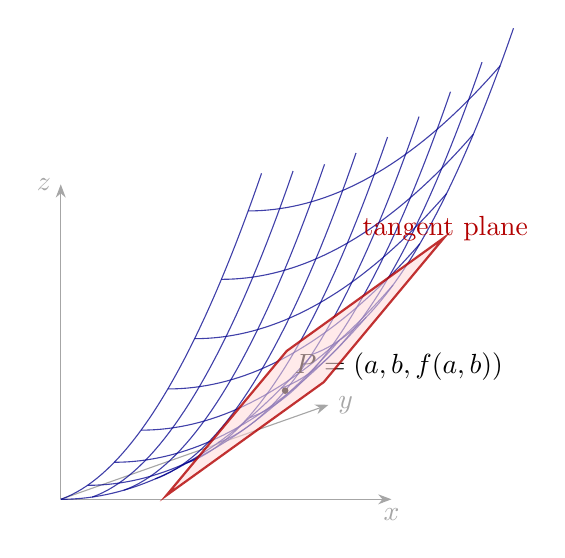
\begin{tikzpicture}[scale=1.0,
  x={(1.0cm,0.0cm)},
  y={(0.85cm,0.30cm)},
  z={(0.0cm,1.0cm)}]

  % axes
  \draw[-{Stealth},gray!70] (0,0,0) -- (4.2,0,0) node[below] {$x$};
  \draw[-{Stealth},gray!70] (0,0,0) -- (0,4.0,0) node[right] {$y$};
  \draw[-{Stealth},gray!70] (0,0,0) -- (0,0,4.0) node[left] {$z$};

  % surface: z = 0.18 x^2 + 0.36 y^2 over [0,3.2]x[0,3.0]
  \foreach \u in {0,0.4,...,3.2} {
    \draw[blue!55!black,opacity=0.75]
      plot[variable=\v,domain=0:3.0,samples=40]
      ({\u},{\v},{0.18*(\u*\u)+0.36*(\v*\v)});
  }
  \foreach \v in {0,0.4,...,3.0} {
    \draw[blue!55!black,opacity=0.75]
      plot[variable=\u,domain=0:3.2,samples=40]
      ({\u},{\v},{0.18*(\u*\u)+0.36*(\v*\v)});
  }

  % point (a,b) = (2,1)
  \pgfmathsetmacro{\a}{2.0}
  \pgfmathsetmacro{\b}{1.0}
  \pgfmathsetmacro{\zab}{0.18*(\a*\a)+0.36*(\b*\b)}
  \coordinate (P) at (\a,\b,\zab);
  \fill (P) circle (1.2pt);
  \node[above right] at (P) {$P=(a,b,f(a,b))$};

  % tangent plane at (2,1): f_x = 0.36 x, f_y = 0.72 y so at (2,1): fx=0.72, fy=0.72
  % plane: z = f(a,b) + fx(x-a) + fy(y-b)
  % draw a parallelogram patch of the plane
  \coordinate (A) at (1.0,0.4,{ \zab + 0.72*(1.0-\a) + 0.72*(0.4-\b)});
  \coordinate (B) at (3.0,0.4,{ \zab + 0.72*(3.0-\a) + 0.72*(0.4-\b)});
  \coordinate (C) at (3.0,2.2,{ \zab + 0.72*(3.0-\a) + 0.72*(2.2-\b)});
  \coordinate (D) at (1.0,2.2,{ \zab + 0.72*(1.0-\a) + 0.72*(2.2-\b)});

  \fill[red!15,opacity=0.55] (A)--(B)--(C)--(D)--cycle;
  \draw[red!70!black,thick,opacity=0.8] (A)--(B)--(C)--(D)--cycle;
  \node[red!70!black] at (2.8,2.45,{ \zab + 0.72*(2.8-\a) + 0.72*(2.45-\b)}) {tangent plane};

\end{tikzpicture}
\caption{A surface patch and its tangent plane at a point: the plane is the best local linear fit.}
\label{fig:tangent-plane-3d}
\end{figure}

\subsubsection{Linearization (Best Local Linear Approximation)}

\begin{definition}[Linearization]\label{def:linearization}
If $f$ is differentiable at $(a,b)$, its \emph{linearization} at $(a,b)$ is the linear function
\begin{equation}\label{eq:linearization}
L(x,y)= f(a,b) + f_x(a,b)(x-a) + f_y(a,b)(y-b).
\end{equation}
Then $f(x,y)\approx L(x,y)$ for $(x,y)$ near $(a,b)$.
\end{definition}

\begin{remark}[What you should remember]
Linearization is “tangent plane as a formula.”  
When you need a quick approximation, compute $f(a,b)$ and the two partial derivatives there, and plug into \cref{eq:linearization}.
\end{remark}

\begin{example}[Fast approximation with small changes]
Approximate $\sqrt{(4.02)^2 + (0.01)^2}$ without a calculator.

Let $f(x,y)=\sqrt{x^2+y^2}$ and expand near $(a,b)=(4,0)$.  
Compute:
\[
f(4,0)=4,\qquad
f_x(x,y)=\frac{x}{\sqrt{x^2+y^2}},\qquad
f_y(x,y)=\frac{y}{\sqrt{x^2+y^2}}.
\]
So $f_x(4,0)=1$ and $f_y(4,0)=0$. Then
\[
L(x,y)=4+1(x-4)+0(y-0)=x.
\]
Now take $(x,y)=(4.02,0.01)$:
\[
f(4.02,0.01)\approx L(4.02,0.01)=4.02.
\]
(The $y$-change contributes only at second order because $f_y(4,0)=0$.)
\end{example}

\subsubsection{Error Estimates (Second-Order Control)}

\begin{theorem}[Second-order Taylor form with remainder]\label{thm:taylor-2var}
Assume $f$ has continuous second partial derivatives on a neighborhood of $(a,b)$.  
For $(x,y)=(a+h,b+k)$ near $(a,b)$, there exist points along the line segment from $(a,b)$ to $(a+h,b+k)$ such that
\begin{equation}\label{eq:taylor-2var}
f(a+h,b+k)=f(a,b)+f_x(a,b)h+f_y(a,b)k+\frac12\Big(f_{xx}(\xi,\eta)h^2+2f_{xy}(\xi,\eta)hk+f_{yy}(\xi,\eta)k^2\Big).
\end{equation}
\end{theorem}

\begin{corollary}[A usable error bound for linearization]\label{cor:error-bound}
Suppose $|f_{xx}|,|f_{xy}|,|f_{yy}| \le M$ on a neighborhood containing the segment from $(a,b)$ to $(x,y)=(a+h,b+k)$.  
Then the linearization error satisfies
\begin{equation}\label{eq:error-bound}
|f(a+h,b+k)-L(a+h,b+k)|
\le \frac{M}{2}\big(|h|+|k|\big)^2
\le M(h^2+k^2).
\end{equation}
\end{corollary}

\begin{proof}
From \cref{eq:taylor-2var}, the error equals the absolute value of the second-order term:
\begin{align*}
\left|\frac12\big(f_{xx}h^2+2f_{xy}hk+f_{yy}k^2\big)\right|
&\le \frac12\Big(|f_{xx}|\,h^2+2|f_{xy}|\,|hk|+|f_{yy}|\,k^2\Big) \\
&\le \frac{M}{2}\big(h^2+2|hk|+k^2\big) \\
&= \frac{M}{2}(|h|+|k|)^2.
\end{align*}
Also $(|h|+|k|)^2 \le 2(h^2+k^2)$, hence the weaker bound $\le M(h^2+k^2)$.
\end{proof}

\begin{exercise}
Let $f(x,y)=e^{x+y}$. Linearize at $(0,0)$ and approximate $e^{0.02-0.01}$.  
Then use \cref{eq:error-bound} with a reasonable bound $M$ on second partial derivatives near $(0,0)$ to estimate the error.
\end{exercise}

% -------------------------------------------------
\subsection{Lesson 4.2: Extrema of Functions of Several Variables}

\subsubsection{Critical Points and Local Extrema}

\begin{definition}[Local maximum/minimum]\label{def:local-extrema}
Let $f:D\subset\RR^2\to\RR$ and $(a,b)\in D$.
\begin{itemize}
\item $f$ has a \emph{local maximum} at $(a,b)$ if $f(a,b)\ge f(x,y)$ for all $(x,y)$ in some neighborhood of $(a,b)$ within $D$.
\item $f$ has a \emph{local minimum} at $(a,b)$ if $f(a,b)\le f(x,y)$ for all $(x,y)$ in some neighborhood of $(a,b)$ within $D$.
\end{itemize}
\end{definition}

\begin{definition}[Critical point]\label{def:critical}
Assume $f_x$ and $f_y$ exist. An interior point $(a,b)$ is a \emph{critical point} if
\[
f_x(a,b)=0 \quad \text{and}\quad f_y(a,b)=0,
\]
or if at least one of $f_x(a,b),f_y(a,b)$ does not exist.
\end{definition}

\begin{theorem}[Fermat's theorem in two variables]\label{thm:fermat}
If $f$ has a local max or local min at an interior point $(a,b)$ and $f_x,f_y$ exist at $(a,b)$, then
\[
f_x(a,b)=0,\qquad f_y(a,b)=0.
\]
\end{theorem}

\begin{remark}[Common pitfall]
\cref{thm:fermat} is one-way: critical points are \emph{candidates} for extrema, not guaranteed extrema.  
You must still classify them (Lesson 4.3) or check boundaries for global problems.
\end{remark}

\subsubsection{Global Extrema on Closed and Bounded Regions}

\begin{theorem}[Extreme Value Theorem (EVT) in $\RR^2$]\label{thm:evt}
If $f$ is continuous on a closed and bounded set $D\subset\RR^2$, then $f$ attains both an absolute maximum and an absolute minimum on $D$.
\end{theorem}

\begin{proposition}[Practical recipe for global extrema]\label{prop:global-recipe}
To find absolute extrema of continuous $f$ on a closed, bounded region $D$:
\begin{enumerate}[label=(\arabic*)]
\item Find all critical points in the interior of $D$ and evaluate $f$ there.
\item Analyze the boundary $\partial D$ (often by parameterizing it or reducing to a single-variable problem) and evaluate $f$ on boundary critical points/endpoints.
\item Compare all values; the largest is the absolute max and the smallest is the absolute min.
\end{enumerate}
\end{proposition}

\begin{example}[Absolute extrema on a disk]
Find the absolute max/min of $f(x,y)=x^2+y^2-2x$ on the closed disk $D=\{(x,y):x^2+y^2\le 4\}$.

\emph{Step 1 (interior critical points).}
\[
f_x=2x-2,\qquad f_y=2y.
\]
Set $f_x=f_y=0$ gives $(x,y)=(1,0)$, which lies in $D$. Then $f(1,0)=1-2=-1$.

\emph{Step 2 (boundary).} On $\partial D$, $x^2+y^2=4$. Then
\[
f=x^2+y^2-2x=4-2x.
\]
So maximizing/minimizing $f$ on the boundary is the same as minimizing/maximizing $x$ on the circle.
On $x^2+y^2=4$, we have $-2\le x\le 2$. Thus
\[
f_{\min,\partial D}=4-2(2)=0 \quad \text{at }(2,0),
\qquad
f_{\max,\partial D}=4-2(-2)=8 \quad \text{at }(-2,0).
\]

\emph{Step 3 (compare).} Candidate values: $-1$ (interior), $0$ and $8$ (boundary).  
So the absolute minimum is $-1$ at $(1,0)$ and the absolute maximum is $8$ at $(-2,0)$.
\end{example}

\begin{exercise}
Find the absolute max and min of $f(x,y)=xy$ on the triangle with vertices $(0,0)$, $(2,0)$, $(0,3)$.
(Hint: boundary consists of three line segments; reduce each to a single-variable function.)
\end{exercise}

% -------------------------------------------------
\subsection{Lesson 4.3: The Second Derivative Test}

\subsubsection{The Hessian Matrix and Quadratic Approximation}

\begin{definition}[Hessian in $\RR^2$]\label{def:hessian}
If $f$ has second partial derivatives, the \emph{Hessian matrix} is
\[
H_f(x,y)=
\begin{pmatrix}
f_{xx}(x,y) & f_{xy}(x,y)\\
f_{yx}(x,y) & f_{yy}(x,y)
\end{pmatrix}.
\]
If the mixed partials are continuous, then $f_{xy}=f_{yx}$ by Clairaut's theorem, so $H_f$ is symmetric.
\end{definition}

\begin{remark}[Why the Hessian matters]
Near a critical point, the first-order (linear) part is zero, so the second-order terms dominate.  
The Hessian tells you whether the surface bends upward (minimum), downward (maximum), or in opposite directions (saddle).
\end{remark}

\subsubsection{Classification in Two Variables}

\begin{theorem}[Second derivative test in $\RR^2$]\label{thm:second-derivative-test}
Let $f$ have continuous second partial derivatives near $(a,b)$, and suppose $(a,b)$ is a critical point with $f_x(a,b)=f_y(a,b)=0$. Define
\begin{equation}\label{eq:D}
D = f_{xx}(a,b)\,f_{yy}(a,b) - \big(f_{xy}(a,b)\big)^2.
\end{equation}
Then:
\begin{enumerate}[label=(\alph*)]
\item If $D>0$ and $f_{xx}(a,b)>0$, then $f$ has a \emph{local minimum} at $(a,b)$.
\item If $D>0$ and $f_{xx}(a,b)<0$, then $f$ has a \emph{local maximum} at $(a,b)$.
\item If $D<0$, then $(a,b)$ is a \emph{saddle point} (neither max nor min).
\item If $D=0$, the test is \emph{inconclusive}.
\end{enumerate}
\end{theorem}

\begin{remark}[In plain language]
$D$ measures whether the quadratic form bends the same way in all directions.  
\begin{itemize}
\item $D>0$ means the quadratic part is definite (up or down), so you get a min or max.
\item $D<0$ means it bends up in some directions and down in others: saddle.
\end{itemize}
\end{remark}

\begin{example}[One min, one saddle, one max]
\begin{enumerate}[label=(\alph*)]
\item $f(x,y)=x^2+y^2$. Critical point at $(0,0)$. Here $f_{xx}=2$, $f_{yy}=2$, $f_{xy}=0$, so $D=4>0$ and $f_{xx}>0$. Local minimum.
\item $g(x,y)=x^2-y^2$. Critical point at $(0,0)$. Here $g_{xx}=2$, $g_{yy}=-2$, $g_{xy}=0$, so $D=-4<0$. Saddle point.
\item $h(x,y)=-(x^2+y^2)$. Critical point at $(0,0)$. Here $h_{xx}=-2$, $h_{yy}=-2$, $h_{xy}=0$, so $D=4>0$ and $h_{xx}<0$. Local maximum.
\end{enumerate}
\end{example}

\begin{figure}[H]
\centering
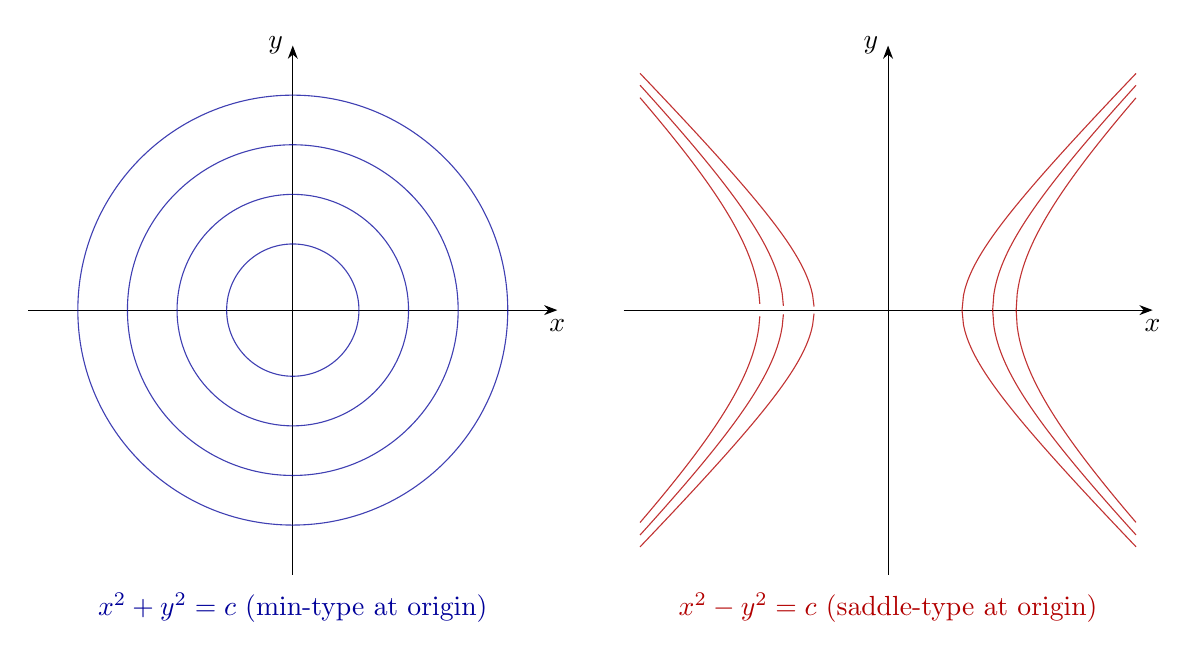
\begin{tikzpicture}[scale=1.05]
  % axes
  \draw[-{Stealth}] (-3.2,0) -- (3.2,0) node[below] {$x$};
  \draw[-{Stealth}] (0,-3.2) -- (0,3.2) node[left] {$y$};

  % level sets for x^2+y^2 = c (min-type)
  \foreach \r in {0.8,1.4,2.0,2.6} {
    \draw[blue!60!black,opacity=0.75] (0,0) circle (\r); 
  }
  \node[blue!60!black] at (0,-3.6) {$x^2+y^2=c$ (min-type at origin)};

  % saddle level sets for x^2-y^2=c (draw a few hyperbolas)
  \begin{scope}[xshift=7.2cm]
    \draw[-{Stealth}] (-3.2,0) -- (3.2,0) node[below] {$x$};
    \draw[-{Stealth}] (0,-3.2) -- (0,3.2) node[left] {$y$};

    \foreach \c in {0.8,1.6,2.4} {
      % 修正说明：加入了 max(0, ...) 以防止浮点数误差导致的负数开根号错误
      
      % 第一象限
      \draw[red!70!black,opacity=0.8]
        plot[variable=\x,domain={sqrt(\c)}:3.0,samples=120]
        ({\x},{sqrt(max(0, \x*\x-\c))});
        
      % Fourth Quadrant (y is negative)
      \draw[red!70!black,opacity=0.8]
        plot[variable=\x,domain={sqrt(\c)}:3.0,samples=120]
        ({\x},{-sqrt(max(0, \x*\x-\c))});
        
      % Second Quadrant (x is negative)
      \draw[red!70!black,opacity=0.8]
        plot[variable=\x,domain={-3.0}:{-sqrt(\c)},samples=120]
        ({\x},{sqrt(max(0, \x*\x-\c))});
        
      % Third Quadrant (x and y are negative)
      \draw[red!70!black,opacity=0.8]
        plot[variable=\x,domain={-3.0}:{-sqrt(\c)},samples=120]
        ({\x},{-sqrt(max(0, \x*\x-\c))});
    }
    \node[red!70!black] at (0,-3.6) {$x^2-y^2=c$ (saddle-type at origin)};
  \end{scope}
\end{tikzpicture}
\caption{Contour patterns distinguish local minima (nested ovals) from saddles (hyperbolic contours).}
\label{fig:contour-shapes}
\end{figure}

\begin{exercise}
Classify all critical points of $f(x,y)=x^3-3x+y^2$ using \cref{thm:second-derivative-test}.  
(Compute $f_x,f_y$, solve for critical points, then compute $D$.)
\end{exercise}

% -------------------------------------------------
\subsection{Lesson 4.4: Constrained Optimization}

\subsubsection{Lagrange Multipliers: Statement}

\begin{theorem}[Lagrange multipliers (one constraint)]\label{thm:lagrange}
Let $f,g:\RR^2\to\RR$ have continuous partial derivatives. Suppose $f$ has a local maximum or minimum on the constraint curve
\[
g(x,y)=c
\]
at a point $(a,b)$ where $\nabla g(a,b)\neq \vect 0$. Then there exists a scalar $\lambda$ such that
\begin{equation}\label{eq:lagrange}
\nabla f(a,b)=\lambda\,\nabla g(a,b).
\end{equation}
\end{theorem}

\begin{remark}[Geometric meaning (the one picture to remember)]
Along the constraint $g=c$, you are allowed to move only \emph{tangent} to the curve.  
At an extremum, moving tangent should not change $f$ (no first-order increase/decrease).  
That means $\nabla f$ must be perpendicular to the tangent direction.  
But $\nabla g$ is also perpendicular to the constraint curve (it is normal to $g=c$).  
So the two normals are parallel: $\nabla f=\lambda \nabla g$.
\end{remark}

\begin{figure}[H]
\centering
\begin{tikzpicture}[scale=1.05]
  % axes
  \draw[-{Stealth}] (-3.2,0) -- (3.2,0) node[below] {$x$};
  \draw[-{Stealth}] (0,-3.2) -- (0,3.2) node[left] {$y$};

  % constraint: circle g=x^2+y^2=4
  \draw[thick,blue!60!black] (0,0) circle (2);

  % Tangency point
  \pgfmathsetmacro{\srt}{1.41421356}
  \coordinate (P) at (\srt,\srt);
  
  % 修改1：移动 P 点标签位置，避免挡住向量
  \fill (P) circle (1.5pt);
  \node[left=3pt] at (P) {$P$};

  % line x+y = 2*sqrt(2)
  \draw[thick,red!70!black] (-3, {2*\srt+3}) -- (3, {2*\srt-3});
  \node[red!70!black] at (-2.5,2.9) {$f=\text{const}$};

  % --- 梯度向量修正 ---
  
  % gradient of g (Constraint): 画长一点 (length ~1.1)，标签放左上
  \draw[-{Stealth},thick,blue!60!black] (P) -- ({\srt+1.1},{\srt+1.1}) 
       node[above left, inner sep=1pt] {$\nabla g$};

  % gradient of f (Objective): 画短一点 (length ~0.6)，标签放右下
  \draw[-{Stealth},thick,red!70!black] (P) -- ({\srt+0.6},{\srt+0.6}) 
       node[below right, inner sep=1pt] {$\nabla f$};

  % -------------------

  % tangent direction
  \draw[-{Stealth},thick,green!50!black] (P) -- ({\srt-0.9},{\srt+0.9}) 
       node[left] {tangent};

  \node at (0,-3.8) {At the optimum on $g=c$, the level curve of $f$ is tangent to the constraint.};
\end{tikzpicture}
\caption{Lagrange multipliers: at a constrained extremum, $\nabla f$ and $\nabla g$ are parallel.}
\label{fig:lagrange-geom}
\end{figure}

\subsubsection{How to Use Lagrange Multipliers (Algorithm)}

\begin{proposition}[Computational procedure]\label{prop:lagrange-proc}
To optimize $f(x,y)$ subject to $g(x,y)=c$:
\begin{enumerate}[label=(\arabic*)]
\item Compute gradients $\nabla f=\langle f_x,f_y\rangle$ and $\nabla g=\langle g_x,g_y\rangle$.
\item Solve the system
\[
\nabla f(x,y)=\lambda \nabla g(x,y),\qquad g(x,y)=c
\]
for $(x,y,\lambda)$.
\item Evaluate $f$ at the candidate points and decide which are max/min (often by comparison, or using context).
\end{enumerate}
\end{proposition}

\subsubsection{Worked Examples}

\begin{example}[Max/min of a product on a circle]
Find the maximum and minimum of $f(x,y)=xy$ subject to $g(x,y)=x^2+y^2=1$.

Compute gradients:
\[
\nabla f=\langle y,\ x\rangle,\qquad \nabla g=\langle 2x,\ 2y\rangle.
\]
Set $\nabla f=\lambda \nabla g$:
\[
y=2\lambda x,\qquad x=2\lambda y,\qquad x^2+y^2=1.
\]
If $x=0$, then $y^2=1$ so $y=\pm 1$, and $f=0$.
If $x\neq 0$ and $y\neq 0$, substitute $y=2\lambda x$ into $x=2\lambda y$:
\[
x=2\lambda(2\lambda x)=4\lambda^2 x \quad\Rightarrow\quad 4\lambda^2=1 \Rightarrow \lambda=\pm\frac12.
\]
If $\lambda=\tfrac12$, then $y=x$ and $x^2+y^2=2x^2=1$, so $x=\pm\frac{1}{\sqrt2}$ and $y=\pm\frac{1}{\sqrt2}$ (same sign). Then $f=xy=\frac12$.
If $\lambda=-\tfrac12$, then $y=-x$ and $2x^2=1$, so $x=\pm\frac{1}{\sqrt2}$ and $y=\mp\frac{1}{\sqrt2}$ (opposite signs). Then $f=-\frac12$.

So the maximum is $\frac12$ at $\left(\frac{1}{\sqrt2},\frac{1}{\sqrt2}\right)$ and $\left(-\frac{1}{\sqrt2},-\frac{1}{\sqrt2}\right)$,
and the minimum is $-\frac12$ at $\left(\frac{1}{\sqrt2},-\frac{1}{\sqrt2}\right)$ and $\left(-\frac{1}{\sqrt2},\frac{1}{\sqrt2}\right)$.
\end{example}

\begin{example}[Distance to a line: closest point]
Find the point on the line $x+y=1$ closest to the origin.

Minimize squared distance $f(x,y)=x^2+y^2$ subject to $g(x,y)=x+y=1$.
\[
\nabla f=\langle 2x,2y\rangle,\qquad \nabla g=\langle 1,1\rangle.
\]
Set $\nabla f=\lambda \nabla g$:
\[
2x=\lambda,\qquad 2y=\lambda,\qquad x+y=1.
\]
Thus $x=y$, so $2x=1$ and $x=y=\frac12$.
The closest point is $\left(\frac12,\frac12\right)$, and the minimum distance is $\sqrt{\left(\frac12\right)^2+\left(\frac12\right)^2}=\frac{1}{\sqrt2}$.
\end{example}

\begin{exercise}
Use Lagrange multipliers to find the maximum and minimum of $f(x,y)=x^2+2y^2$ subject to $x^2+y^2=3$.  
(Your final answers should be specific points and corresponding max/min values.)
\end{exercise}

\subsubsection*{Chapter 4 Checklist}
\begin{itemize}
\item Tangent plane / linearization at $(a,b)$:
\[
L(x,y)=f(a,b)+f_x(a,b)(x-a)+f_y(a,b)(y-b).
\]
\item Use second derivatives to control approximation error (Taylor + bounds) \cref{cor:error-bound}.
\item Local extrema candidates: interior critical points \cref{def:critical}; global extrema on closed bounded sets via EVT \cref{thm:evt}.
\item Classify critical points using the second derivative test \cref{thm:second-derivative-test}.
\item Constrained optimization: solve $\nabla f=\lambda \nabla g$ plus the constraint equation \cref{thm:lagrange}.
\end{itemize}

% =========================
% End of Chapter 4
% =========================

% =========================
% Chapter 5 (no preamble)
% =========================

\section{Chapter 5: Multiple Integrals}

\begin{keyidea}
Single-variable integration adds up tiny \emph{line segments}.  
Double integrals add up tiny \emph{area elements} $dA$ over a region in the plane.  
Triple integrals add up tiny \emph{volume elements} $dV$ over a region in space.  

The most intuitive understanding: divide a region into many very small pieces (small rectangles/small boxes), on each small piece compute "function value $\times$ area/volume of small piece", then add them all up—the limit is the multiple integral.
\end{keyidea}

% -------------------------------------------------
\subsection{Lesson 5.1: Double Integrals over Rectangular Regions}

\subsubsection{Definition of Double Integrals}

\begin{definition}[Double integral over a rectangle]\label{def:double-rect}
Let $R=[a,b]\times[c,d]\subset\RR^2$ and let $f$ be bounded on $R$.
Partition $[a,b]$ into $m$ subintervals and $[c,d]$ into $n$ subintervals, forming subrectangles
\[
R_{ij}=[x_{i-1},x_i]\times[y_{j-1},y_j],\qquad
\Delta A_{ij}=(x_i-x_{i-1})(y_j-y_{j-1}).
\]
Choose a sample point $(x_{ij}^*,y_{ij}^*)\in R_{ij}$ and form the Riemann sum
\[
S=\sum_{i=1}^{m}\sum_{j=1}^{n} f(x_{ij}^*,y_{ij}^*)\,\Delta A_{ij}.
\]
If $S$ approaches a limit as $\max\{\Delta x_i,\Delta y_j\}\to 0$ (independent of sample points), then $f$ is \emph{integrable} on $R$ and we define
\[
\iint_R f(x,y)\,dA=\lim_{\max\{\Delta x_i,\Delta y_j\}\to 0}\sum_{i=1}^{m}\sum_{j=1}^{n} f(x_{ij}^*,y_{ij}^*)\,\Delta A_{ij}.
\]
\end{definition}

\begin{remark}[A safe existence condition]
If $f$ is continuous on the rectangle $R$, then $f$ is integrable on $R$ and the double integral exists.
\end{remark}

\begin{figure}[H]
\centering
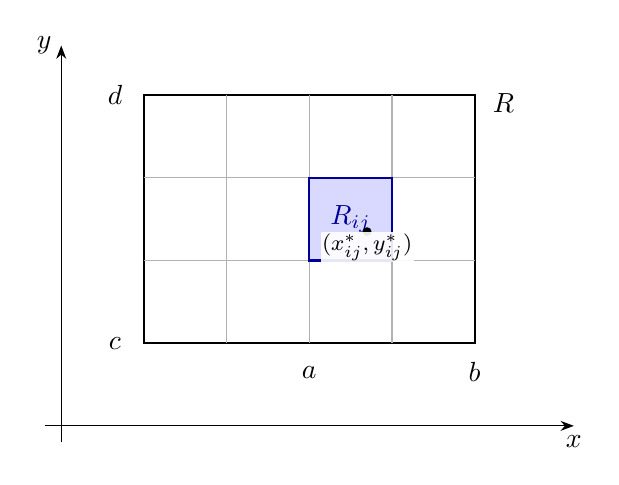
\begin{tikzpicture}[scale=1.05]
  % axes
  \draw[-{Stealth}] (-0.2,0) -- (6.2,0) node[below] {$x$};
  \draw[-{Stealth}] (0,-0.2) -- (0,4.6) node[left] {$y$};

  % rectangle R: [1,5]x[1,4]
  \draw[thick] (1,1) rectangle (5,4);
  \node at (5.35,3.9) {$R$};

  % partition grid
  \foreach \x in {2,3,4} {
    \draw[gray!60] (\x,1) -- (\x,4);
  }
  \foreach \y in {2,3} {
    \draw[gray!60] (1,\y) -- (5,\y);
  }

  % highlight one subrectangle
  \fill[blue!15] (3,2) rectangle (4,3);
  \draw[blue!60!black,thick] (3,2) rectangle (4,3);
  \node[blue!60!black] at (3.5,2.5) {$R_{ij}$};

  % sample point
  \fill (3.7,2.35) circle (1.5pt);
  % --- 修复部分开始 ---
  % 将标签移到点下方，缩小字体，并增加白色背景以提高清晰度
  \node[below, fill=white, inner sep=0.5pt, opacity=0.9, text opacity=1, font=\footnotesize] at (3.7,2.35) {$(x^*_{ij},y^*_{ij})$};
  % --- 修复部分结束 ---

  % labels
  \node at (3,0.65) {$a$}; % 稍微调整了下位置，更对齐网格线
  \node at (5,0.65) {$b$};
  \node at (0.65,1) {$c$};
  \node at (0.65,4) {$d$};
\end{tikzpicture}
\caption{A rectangle region partitioned into small subrectangles $R_{ij}$; the double integral is the limit of sums $f(x^*_{ij},y^*_{ij})\Delta A_{ij}$.}
\label{fig:double-riemann}
\end{figure}

\subsubsection{Iterated Integrals}

\begin{theorem}[Iterated integral over a rectangle]\label{thm:iterated-rect}
If $f$ is continuous on $R=[a,b]\times[c,d]$, then
\begin{equation}\label{eq:iterated-rect}
\iint_R f(x,y)\,dA=\int_{a}^{b}\left(\int_{c}^{d} f(x,y)\,dy\right)\,dx
=\int_{c}^{d}\left(\int_{a}^{b} f(x,y)\,dx\right)\,dy.
\end{equation}
\end{theorem}

\begin{remark}[Intuitive understanding]
In a rectangular region, you can first "add up each vertical strip in the $y$ direction" (inner integral), then sum all the vertical strips over $x$ (outer integral).  
You can also reverse the order: first along $x$ then along $y$. The advantage of rectangles is that the upper, lower, left, and right boundaries are all constants.
\end{remark}

\begin{example}[Compute a double integral on a rectangle]
Let $R=[0,1]\times[0,2]$ and $f(x,y)=x+y$. Then
\[
\iint_R (x+y)\,dA=\int_{0}^{1}\int_{0}^{2}(x+y)\,dy\,dx.
\]
Compute the inner integral:
\[
\int_{0}^{2}(x+y)\,dy=\Big(xy+\tfrac12 y^2\Big)\Big|_{0}^{2}=2x+2.
\]
Then
\[
\int_{0}^{1}(2x+2)\,dx=\big(x^2+2x\big)\Big|_{0}^{1}=1+2=3.
\]
So $\iint_R (x+y)\,dA=3$.
\end{example}

\subsubsection{Fubini's Theorem}

\begin{theorem}[Fubini's Theorem (practical version)]\label{thm:fubini}
If $f$ is continuous on a rectangle $R$, then both iterated integrals in \cref{eq:iterated-rect} exist and are equal to $\iint_R f\,dA$.
More generally, if $\iint_R |f|\,dA<\infty$ (absolute integrability), then the iterated integrals exist and are equal.
\end{theorem}

\begin{exercise}
Compute $\iint_{[1,3]\times[0,1]} (2x-3y)\,dA$ in two ways:
\[
\int_{1}^{3}\int_{0}^{1}(2x-3y)\,dy\,dx
\quad\text{and}\quad
\int_{0}^{1}\int_{1}^{3}(2x-3y)\,dx\,dy.
\]
Verify the answers match.
\end{exercise}

% -------------------------------------------------
\subsection{Lesson 5.2: Double Integrals over General Regions}

\subsubsection{Type I and Type II Regions}

\begin{definition}[Type I (vertically simple) region]\label{def:typeI}
A region $D\subset\RR^2$ is \emph{Type I} if it can be described as
\[
D=\{(x,y): a\le x\le b,\ g_1(x)\le y\le g_2(x)\},
\]
for some functions $g_1,g_2$ with $g_1(x)\le g_2(x)$ on $[a,b]$.
\end{definition}

\begin{definition}[Type II (horizontally simple) region]\label{def:typeII}
A region $D\subset\RR^2$ is \emph{Type II} if it can be described as
\[
D=\{(x,y): c\le y\le d,\ h_1(y)\le x\le h_2(y)\},
\]
for some functions $h_1,h_2$ with $h_1(y)\le h_2(y)$ on $[c,d]$.
\end{definition}

\begin{theorem}[Integrating over Type I / Type II regions]\label{thm:typeI-II-integrals}
If $f$ is continuous on $D$, then
\[
\iint_D f(x,y)\,dA=\int_{a}^{b}\int_{g_1(x)}^{g_2(x)} f(x,y)\,dy\,dx
\quad (\text{Type I}),
\]
\[
\iint_D f(x,y)\,dA=\int_{c}^{d}\int_{h_1(y)}^{h_2(y)} f(x,y)\,dx\,dy
\quad (\text{Type II}).
\]
\end{theorem}

\begin{remark}[Intuitive understanding]
Type I: use "vertical slices," fix $x$, $y$ goes from lower boundary $g_1(x)$ to upper boundary $g_2(x)$.  
Type II: use "horizontal slices," fix $y$, $x$ goes from left boundary $h_1(y)$ to right boundary $h_2(y)$.  
The same region can often be represented using either Type I or Type II; choose whichever is simpler.
\end{remark}

\begin{figure}[H]
\centering
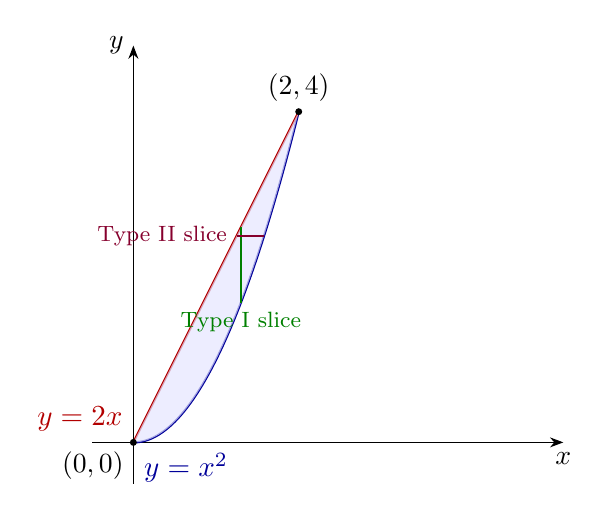
\begin{tikzpicture}[scale=1.05]
  % axes
  \draw[-{Stealth}] (-0.5,0) -- (5.2,0) node[below] {$x$};
  \draw[-{Stealth}] (0,-0.5) -- (0,4.8) node[left] {$y$};

  % curves y = x^2 and y = 2x
  % 修改1：使用 pos=0.5 将标签放在曲线中段，避开端点
  \draw[thick,blue!60!black,domain=0:2,samples=150]
    plot (\x,{\x*\x}) node[pos=0.5, below right] {$y=x^2$};
    
  % 修改2：使用 sloped 让标签跟随直线斜率，并放在中段
  \draw[thick,red!70!black,domain=0:2,samples=2]
    plot (\x,{2*\x}) node[pos=0.6, above left, sloped] {$y=2x$};

  % shading region
  \fill[blue!10,opacity=0.7]
    (0,0) --
    plot[domain=0:2,samples=150] (\x,{2*\x}) --
    (2,4) --
    plot[domain=2:0,samples=150] (\x,{\x*\x}) -- cycle;

  % --- Slices (切片) ---

  % vertical slice at x=1.3 (Type I)
  \draw[thick,green!50!black] (1.3,{1.3*1.3}) -- (1.3,{2*1.3});
  % 修改3：将标签移到切片底部，利用抛物线下方的空白
  \node[green!50!black, below, font=\footnotesize] at (1.3, {1.3*1.3}) {Type I slice};

  % horizontal slice at y=2.5 (Type II)
  \pgfmathsetmacro{\yy}{2.5}
  \draw[thick,purple!70!black] ({\yy/2},\yy) -- ({sqrt(\yy)},\yy);
  % 修改4：将标签移到切片左侧，利用直线左侧的空白
  \node[purple!70!black, left, font=\footnotesize] at ({\yy/2},\yy) {Type II slice};

  % intersection points
  \fill (0,0) circle (1.2pt);
  \fill (2,4) circle (1.2pt);
  \node[below left] at (0,0) {$(0,0)$};
  % 修改5：(2,4) 标签单独放在上方，不再和曲线名打架
  \node[above] at (2,4) {$(2,4)$};
\end{tikzpicture}
\caption{A region that is both Type I and Type II: between $y=x^2$ and $y=2x$ in the first quadrant.}
\label{fig:typeI-typeII}
\end{figure}

\subsubsection{Changing the Order of Integration}

\begin{proposition}[How to change the order (workflow)]\label{prop:change-order}
Given an iterated integral, to switch $dy\,dx$ to $dx\,dy$ (or vice versa):
\begin{enumerate}[label=(\arabic*)]
\item Sketch the region $D$ described by the current bounds.
\item Decide whether you want vertical slices (Type I) or horizontal slices (Type II).
\item Rewrite $D$ with the new slice description (new outer bounds + new inner bounds).
\item Rewrite the integral with the new bounds; then integrate.
\end{enumerate}
\end{proposition}

\begin{example}[Change order for the region between $y=x^2$ and $y=2x$]
Let $D=\{(x,y):0\le x\le 2,\ x^2\le y\le 2x\}$.
Then
\[
\iint_D 1\,dA=\int_{0}^{2}\int_{x^2}^{2x} 1\,dy\,dx.
\]
Compute directly:
\[
\int_{0}^{2}\big(2x-x^2\big)\,dx=\Big(x^2-\tfrac13 x^3\Big)\Big|_{0}^{2}=4-\tfrac83=\tfrac{4}{3}.
\]

Now rewrite as Type II. Here $y$ ranges from $0$ to $4$. For a fixed $y\in[0,4]$, $x$ runs from the line $y=2x$ (i.e.\ $x=y/2$) to the parabola $y=x^2$ (i.e.\ $x=\sqrt{y}$):
\[
D=\{(x,y):0\le y\le 4,\ \tfrac{y}{2}\le x\le \sqrt{y}\}.
\]
Thus
\[
\iint_D 1\,dA=\int_{0}^{4}\int_{y/2}^{\sqrt{y}} 1\,dx\,dy
=\int_{0}^{4}\left(\sqrt{y}-\frac{y}{2}\right)\,dy
=\left(\frac{2}{3}y^{3/2}-\frac14 y^2\right)\Big|_{0}^{4}
=\frac{16}{3}-4=\frac{4}{3},
\]
which matches, as it must.
\end{example}

\begin{exercise}
Rewrite and evaluate
\[
\int_{0}^{1}\int_{x}^{1} e^{y^2}\,dy\,dx
\]
by switching the order of integration. (Hint: the integrand suggests $dx$ inside.)
\end{exercise}

% -------------------------------------------------
\subsection{Lesson 5.3: Applications of Double Integrals}

\subsubsection{Area and Volume}

\begin{proposition}[Area of a planar region]\label{prop:area}
If $D\subset\RR^2$ is a region with finite area, then
\[
\operatorname{Area}(D)=\iint_D 1\,dA.
\]
\end{proposition}

\begin{proposition}[Volume under a surface]\label{prop:volume-under}
If $f(x,y)\ge 0$ on $D$, then the volume under $z=f(x,y)$ above $D$ is
\[
V=\iint_D f(x,y)\,dA.
\]
If $f$ changes sign, $\iint_D f\,dA$ is a \emph{signed volume}; geometric volume is typically $\iint_D |f|\,dA$.
\end{proposition}

\begin{remark}[Intuitive understanding]
$\iint_D 1\,dA$ is "counting each small area element once," so it yields the total area.  
$\iint_D f\,dA$ is multiplying the "height $f$" of each small piece by its "base area $dA$," and adding them up gives the volume (when $f\ge0$).
\end{remark}

\subsubsection{Mass and Density}

\begin{proposition}[Mass of a lamina]\label{prop:mass}
If a thin plate occupies region $D$ with (possibly varying) surface density $\rho(x,y)\ge 0$ (mass per unit area), then its mass is
\[
m=\iint_D \rho(x,y)\,dA.
\]
\end{proposition}

\subsubsection{Average Value}

\begin{definition}[Average value on a region]\label{def:avg-value}
If $f$ is integrable on $D$ and $\operatorname{Area}(D)>0$, the average value of $f$ on $D$ is
\[
f_{\text{avg}}=\frac{1}{\operatorname{Area}(D)}\iint_D f(x,y)\,dA.
\]
\end{definition}

\begin{example}[Mass with variable density on a triangular region]
Let $D=\{(x,y): 0\le x\le 1,\ 0\le y\le 2x\}$ (a triangle).
Let density be $\rho(x,y)=x+y$. Then
\[
m=\iint_D (x+y)\,dA=\int_{0}^{1}\int_{0}^{2x} (x+y)\,dy\,dx.
\]
Compute the inner integral:
\[
\int_{0}^{2x}(x+y)\,dy=\Big(xy+\tfrac12 y^2\Big)\Big|_{0}^{2x}=2x^2+2x^2=4x^2.
\]
Then
\[
m=\int_{0}^{1}4x^2\,dx=\frac{4}{3}.
\]
Also $\operatorname{Area}(D)=\int_{0}^{1}\int_{0}^{2x}1\,dy\,dx=\int_{0}^{1}2x\,dx=1$.
So the average density (and the average of $x+y$ over $D$) is $m/\operatorname{Area}(D)=\frac{4}{3}$.
\end{example}

\begin{example}[Average value over a rectangle]
Let $R=[0,2]\times[0,1]$ and $f(x,y)=x^2+2y$.
\begin{align*}
\iint_R f\,dA &= \int_{0}^{2}\int_{0}^{1}(x^2+2y)\,dy\,dx 
= \int_{0}^{2}\Big(x^2y+y^2\Big)\Big|_{0}^{1}\,dx \\
&= \int_{0}^{2}(x^2+1)\,dx 
= \Big(\tfrac13 x^3+x\Big)\Big|_{0}^{2}
= \frac{8}{3}+2=\frac{14}{3}.
\end{align*}
Area$(R)=2$. Hence
\[
f_{\text{avg}}=\frac{1}{2}\cdot\frac{14}{3}=\frac{7}{3}.
\]
\end{example}

\begin{exercise}
Find the volume under $z=3-x-y$ above the triangle with vertices $(0,0)$, $(3,0)$, $(0,2)$.
(First confirm $3-x-y\ge0$ on the region.)
\end{exercise}

% -------------------------------------------------
\subsection{Lesson 5.4: Polar Coordinates}

\subsubsection{Polar Coordinate System}

\begin{definition}[Polar coordinates]\label{def:polar}
Polar coordinates represent a point in the plane by $(r,\theta)$ where
\[
x=r\cos\theta,\qquad y=r\sin\theta,\qquad r\ge 0.
\]
Also
\[
r=\sqrt{x^2+y^2},\qquad \theta=\text{angle from the positive $x$-axis (chosen consistently).}
\]
\end{definition}

\begin{proposition}[Area element in polar coordinates]\label{prop:polar-area}
Under the change of variables $(x,y)=(r\cos\theta,r\sin\theta)$, the area element transforms as
\begin{equation}\label{eq:polar-jac}
dA = r\,dr\,d\theta.
\end{equation}
\end{proposition}

\begin{remark}[Intuitive understanding]
At a fixed angle $\theta$, as the radius increases from $r$ to $r+dr$, it forms a "thin annular wedge" with area approximately
\[
(\text{arc length})\times(\text{thickness}) \approx (r\,d\theta)\cdot(dr)=r\,dr\,d\theta,
\]
which is the extra factor of $r$ in \cref{eq:polar-jac}.
\end{remark}

\begin{figure}[H]
\centering
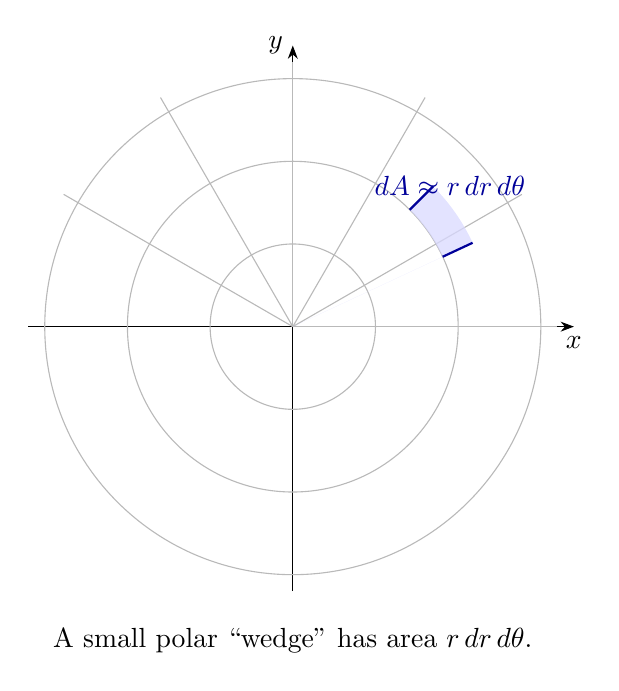
\begin{tikzpicture}[scale=1.05]
  % axes
  \draw[-{Stealth}] (-3.2,0) -- (3.4,0) node[below] {$x$};
  \draw[-{Stealth}] (0,-3.2) -- (0,3.4) node[left] {$y$};

  % polar grid (a few circles)
  \foreach \r in {1,2,3} {
    \draw[gray!55] (0,0) circle (\r);
  }
  \foreach \ang in {0,30,...,150} {
    \draw[gray!55] (0,0) -- ({3.2*cos(\ang)},{3.2*sin(\ang)});
  }

  % wedge element
  \fill[blue!15,opacity=0.75]
    (0,0) --
    ({2.0*cos(25)},{2.0*sin(25)}) --
    ({2.4*cos(25)},{2.4*sin(25)}) arc[start angle=25,end angle=45,radius=2.4] --
    ({2.0*cos(45)},{2.0*sin(45)}) arc[start angle=45,end angle=25,radius=2.0] -- cycle;

  \draw[blue!60!black,thick]
    ({2.0*cos(25)},{2.0*sin(25)}) -- ({2.4*cos(25)},{2.4*sin(25)});
  \draw[blue!60!black,thick]
    ({2.0*cos(45)},{2.0*sin(45)}) -- ({2.4*cos(45)},{2.4*sin(45)});

  \node[blue!60!black] at (1.9,1.7) {$dA\approx r\,dr\,d\theta$};
  \node at (0,-3.8) {A small polar ``wedge'' has area $r\,dr\,d\theta$.};
\end{tikzpicture}
\caption{Polar coordinates: the Jacobian factor $r$ comes from the arc length $r\,d\theta$.}
\label{fig:polar-wedge}
\end{figure}

\subsubsection{Double Integrals in Polar Coordinates}

\begin{theorem}[Polar-coordinate double integral]\label{thm:polar-double}
Let $D$ be described in polar form by
\[
\alpha\le \theta\le \beta,\qquad 0\le r\le g(\theta),
\]
and let $f$ be integrable on $D$. Then
\begin{equation}\label{eq:polar-double}
\iint_D f(x,y)\,dA
=
\int_{\alpha}^{\beta}\int_{0}^{g(\theta)}
f(r\cos\theta,r\sin\theta)\, r\,dr\,d\theta.
\end{equation}
More generally, if $r$ ranges between two curves $r=g_1(\theta)$ and $r=g_2(\theta)$, then use $g_1(\theta)\le r\le g_2(\theta)$.
\end{theorem}

\subsubsection{Applications}

\begin{example}[Area of a disk]\label{ex:area-disk}
For the disk $x^2+y^2\le a^2$, we have $0\le r\le a$ and $0\le\theta\le 2\pi$.
Then
\[
\operatorname{Area}=\iint_D 1\,dA
=\int_{0}^{2\pi}\int_{0}^{a} 1\cdot r\,dr\,d\theta
=\int_{0}^{2\pi}\left(\tfrac12 a^2\right)d\theta
=\pi a^2.
\]
\end{example}

\begin{example}[A common integrand: $x^2+y^2$ over a disk]
Let $D=\{(x,y):x^2+y^2\le a^2\}$ and $f(x,y)=x^2+y^2$.
In polar, $f=r^2$. Thus
\[
\iint_D (x^2+y^2)\,dA
=\int_{0}^{2\pi}\int_{0}^{a} r^2\cdot r\,dr\,d\theta
=\int_{0}^{2\pi}\int_{0}^{a} r^3\,dr\,d\theta
=\int_{0}^{2\pi}\left(\tfrac14 a^4\right)d\theta
=\frac{\pi}{2}a^4.
\]
\end{example}

\begin{exercise}
Evaluate $\iint_D \sqrt{x^2+y^2}\,dA$ over the annulus $1\le x^2+y^2\le 4$ using polar coordinates.
\end{exercise}

% -------------------------------------------------
\subsection{Lesson 5.5: Triple Integrals}

\subsubsection{Definition of Triple Integrals}

\begin{definition}[Triple integral over a box]\label{def:triple-box}
Let $B=[a,b]\times[c,d]\times[e,f]\subset\RR^3$, and let $F$ be bounded on $B$.
Partition $B$ into small boxes $B_{ijk}$ with volume $\Delta V_{ijk}$ and choose sample points $(x_{ijk}^*,y_{ijk}^*,z_{ijk}^*)$.
If the Riemann sums
\[
\sum_{i}\sum_{j}\sum_{k} F(x_{ijk}^*,y_{ijk}^*,z_{ijk}^*)\,\Delta V_{ijk}
\]
approach a limit as the mesh goes to $0$, we define
\[
\iiint_B F(x,y,z)\,dV=\lim \sum_{i}\sum_{j}\sum_{k} F(x_{ijk}^*,y_{ijk}^*,z_{ijk}^*)\,\Delta V_{ijk}.
\]
\end{definition}

\begin{remark}[Intuitive understanding]
Divide the spatial region into many small boxes, each small box contributes approximately $F\cdot(\text{volume of small box})$, add them all up and take the limit to get the triple integral.
\end{remark}

\subsubsection{Triple Integrals in Rectangular Coordinates (Fubini)}

\begin{theorem}[Iterated integrals for a box]\label{thm:triple-fubini}
If $F$ is continuous on the box $B=[a,b]\times[c,d]\times[e,f]$, then
\[
\iiint_B F(x,y,z)\,dV
=
\int_{a}^{b}\int_{c}^{d}\int_{e}^{f} F(x,y,z)\,dz\,dy\,dx,
\]
and similarly for the other 5 possible integration orders.
\end{theorem}

\subsubsection{Applications to Volume and Mass}

\begin{proposition}[Volume of a solid]\label{prop:volume-solid}
If $E\subset\RR^3$ is a solid region with finite volume, then
\[
\operatorname{Vol}(E)=\iiint_E 1\,dV.
\]
\end{proposition}

\begin{proposition}[Mass of a solid]\label{prop:mass-solid}
If a solid occupies $E$ with density $\rho(x,y,z)\ge 0$ (mass per unit volume), then
\[
m=\iiint_E \rho(x,y,z)\,dV.
\]
\end{proposition}

\begin{definition}[Average value in 3D]\label{def:avg-3d}
If $F$ is integrable on $E$ and $\operatorname{Vol}(E)>0$, then
\[
F_{\text{avg}}=\frac{1}{\operatorname{Vol}(E)}\iiint_E F\,dV.
\]
\end{definition}

\begin{example}[Volume of the tetrahedron $x+y+z\le 1$ in the first octant]\label{ex:tetra-volume}
Let
\[
E=\{(x,y,z): x\ge 0,\ y\ge 0,\ z\ge 0,\ x+y+z\le 1\}.
\]
A convenient description is
\[
0\le x\le 1,\qquad 0\le y\le 1-x,\qquad 0\le z\le 1-x-y.
\]
Thus
\[
\operatorname{Vol}(E)=\iiint_E 1\,dV
=\int_{0}^{1}\int_{0}^{1-x}\int_{0}^{1-x-y} 1\,dz\,dy\,dx.
\]
Integrate:
\[
\int_{0}^{1-x-y}1\,dz=1-x-y,
\]
\[
\int_{0}^{1-x}(1-x-y)\,dy=\Big((1-x)y-\tfrac12 y^2\Big)\Big|_{0}^{1-x}
=\frac{(1-x)^2}{2},
\]
\[
\int_{0}^{1}\frac{(1-x)^2}{2}\,dx
=\frac12\int_{0}^{1}(1-2x+x^2)\,dx
=\frac12\Big(x-x^2+\tfrac13 x^3\Big)\Big|_{0}^{1}
=\frac12\cdot\frac13=\frac{1}{6}.
\]
So $\operatorname{Vol}(E)=\frac{1}{6}$.
\end{example}

\begin{example}[Mass with density $\rho=z$ on the same tetrahedron]\label{ex:tetra-mass}
Using the same region $E$ as \cref{ex:tetra-volume} with density $\rho(x,y,z)=z$,
\[
m=\iiint_E z\,dV
=\int_{0}^{1}\int_{0}^{1-x}\int_{0}^{1-x-y} z\,dz\,dy\,dx.
\]
Compute:
\[
\int_{0}^{1-x-y} z\,dz=\frac{(1-x-y)^2}{2}.
\]
Then
\[
\int_{0}^{1-x}\frac{(1-x-y)^2}{2}\,dy
=\frac12\int_{0}^{1-x} (1-x-y)^2\,dy.
\]
Let $u=1-x-y$ so $du=-dy$, and when $y=0$, $u=1-x$, when $y=1-x$, $u=0$:
\[
\frac12\int_{u=1-x}^{0} u^2(-du)=\frac12\int_{0}^{1-x}u^2\,du=\frac12\cdot\frac{(1-x)^3}{3}=\frac{(1-x)^3}{6}.
\]
Finally
\[
m=\int_{0}^{1}\frac{(1-x)^3}{6}\,dx
=\frac{1}{6}\int_{0}^{1}(1-3x+3x^2-x^3)\,dx
=\frac{1}{6}\left(1-\frac{3}{2}+1-\frac{1}{4}\right)
=\frac{1}{6}\cdot\frac{1}{4}
=\frac{1}{24}.
\]
So $m=\frac{1}{24}$, and the average value of $z$ over $E$ is
\[
z_{\text{avg}}=\frac{m}{\operatorname{Vol}(E)}=\frac{1/24}{1/6}=\frac{1}{4}.
\]
\end{example}

\begin{figure}[H]
\centering
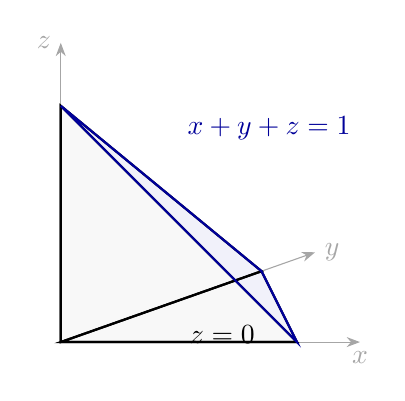
\begin{tikzpicture}[scale=1.0,
  x={(1.0cm,0.0cm)},
  y={(0.85cm,0.30cm)},
  z={(0.0cm,1.0cm)}]

  % axes
  \draw[-{Stealth},gray!70] (0,0,0) -- (3.8,0,0) node[below] {$x$};
  \draw[-{Stealth},gray!70] (0,0,0) -- (0,3.8,0) node[right] {$y$};
  \draw[-{Stealth},gray!70] (0,0,0) -- (0,0,3.8) node[left] {$z$};

  % tetrahedron x+y+z=1 in first octant (scaled for drawing)
  % vertices: (0,0,0), (1,0,0), (0,1,0), (0,0,1)
  \coordinate (O) at (0,0,0);
  \coordinate (X) at (3.0,0,0);
  \coordinate (Y) at (0,3.0,0);
  \coordinate (Z) at (0,0,3.0);

  % faces (light)
  \fill[blue!10,opacity=0.55] (X) -- (Y) -- (Z) -- cycle; % slanted face
  \fill[gray!10,opacity=0.35] (O) -- (X) -- (Y) -- cycle; % z=0 face
  \fill[gray!10,opacity=0.35] (O) -- (X) -- (Z) -- cycle; % y=0 face
  \fill[gray!10,opacity=0.35] (O) -- (Y) -- (Z) -- cycle; % x=0 face

  % edges
  \draw[thick] (O)--(X)--(Y)--cycle;
  \draw[thick] (O)--(X)--(Z)--cycle;
  \draw[thick] (O)--(Y)--(Z)--cycle;
  \draw[thick,blue!60!black] (X)--(Y)--(Z)--cycle;

  \node[blue!60!black] at (1.2,1.7,2.2) {$x+y+z=1$};
  \node at (1.2,1.0,-0.2) {$z=0$};
\end{tikzpicture}
\caption{The solid $x,y,z\ge 0$ and $x+y+z\le 1$ (a tetrahedron). Triple integrals add up $F\,dV$ over such a region.}
\label{fig:tetrahedron}
\end{figure}

\begin{exercise}
Set up (do not necessarily evaluate) an iterated integral for $\iiint_E (x+2y+3z)\,dV$ where $E$ is bounded by
\[
0\le z\le 2,\qquad 0\le y\le 1,\qquad 0\le x\le 3-y.
\]
Then compute the volume of $E$ using $\iiint_E 1\,dV$.
\end{exercise}

\subsubsection*{Chapter 5 Checklist}
\begin{itemize}
\item Double integral definition: limit of sums $f(x^*,y^*)\Delta A$ over partitions (Lesson 5.1).
\item Rectangle $\Rightarrow$ iterated integrals and order swap via Fubini (Theorem \cref{thm:fubini}).
\item General regions: Type I (vertical slices) and Type II (horizontal slices) (Lesson 5.2).
\item Changing order: sketch $D$, rewrite bounds, then integrate (Proposition \cref{prop:change-order}).
\item Applications: area $\iint_D 1\,dA$, volume $\iint_D f\,dA$ (for $f\ge0$), mass $\iint_D \rho\,dA$, average value (Lesson 5.3).
\item Polar coordinates: $(x,y)=(r\cos\theta,r\sin\theta)$ and $dA=r\,dr\,d\theta$ (Lesson 5.4).
\item Triple integrals: $\iiint_E F\,dV$; volume $\iiint_E 1\,dV$; mass $\iiint_E \rho\,dV$ (Lesson 5.5).
\end{itemize}

% =========================
% End of Chapter 5
% =========================

% =========================
% Chapter 6 (no preamble)
% =========================

\section{Chapter 6: Change of Variables in Multiple Integrals}

\begin{keyidea}
A change of variables is the multivariable analogue of substitution in single-variable calculus.

If a mapping $(u,v)\mapsto (x,y)$ is smooth and one-to-one, then small area elements scale by a factor
\[
\left|\frac{\partial(x,y)}{\partial(u,v)}\right|
\]
(the \emph{Jacobian}). This turns complicated regions in the $xy$-plane into simpler regions in the $uv$-plane, where integrals are easier to set up and compute.
\end{keyidea}

% -------------------------------------------------
\subsection{Lesson 6.1: Jacobians and Coordinate Transformations}

\subsubsection{Motivation for Change of Variables}

\begin{remark}[Why we bother]
The hard part of many double/triple integrals is not the integrand; it is the \emph{region}.  
A well-chosen coordinate transformation can turn “curved boundaries” into “constant bounds,” while the Jacobian keeps the calculation honest by correcting the area/volume scale.
\end{remark}

\subsubsection{Transformations and the Jacobian Determinant}

\begin{definition}[Planar transformation]
A (planar) coordinate transformation is a mapping
\[
T:\ (u,v)\mapsto (x,y)=(x(u,v),y(u,v)),
\]
defined on a region $D^\ast$ in the $uv$-plane and mapping it to a region $D=T(D^\ast)$ in the $xy$-plane.
\end{definition}

\begin{definition}[Jacobian determinant]\label{def:jacobian}
Assume $x(u,v)$ and $y(u,v)$ have continuous first partial derivatives. The \emph{Jacobian determinant} of $T$ is
\begin{equation}\label{eq:jacobian}
\frac{\partial(x,y)}{\partial(u,v)}
=
\begin{vmatrix}
x_u & x_v\\
y_u & y_v
\end{vmatrix}
= x_u y_v - x_v y_u.
\end{equation}
\end{definition}

\begin{remark}[Plain-language meaning]
At a point $(u,v)$, the vectors
\[
\vect r_u=\left\langle x_u,\,y_u\right\rangle,\qquad
\vect r_v=\left\langle x_v,\,y_v\right\rangle
\]
approximate how the map moves when you change $u$ or $v$ a little. A tiny $uv$-rectangle with sides $\Delta u$ and $\Delta v$ maps to a tiny parallelogram spanned by $\vect r_u\Delta u$ and $\vect r_v\Delta v$. Its area is approximately
\[
\big|\vect r_u\times \vect r_v\big|
=
\left|x_u y_v-x_v y_u\right|
=
\left|\frac{\partial(x,y)}{\partial(u,v)}\right|.
\]
So the Jacobian is a local \emph{area scale factor}.
\end{remark}

\begin{figure}[H]
\centering
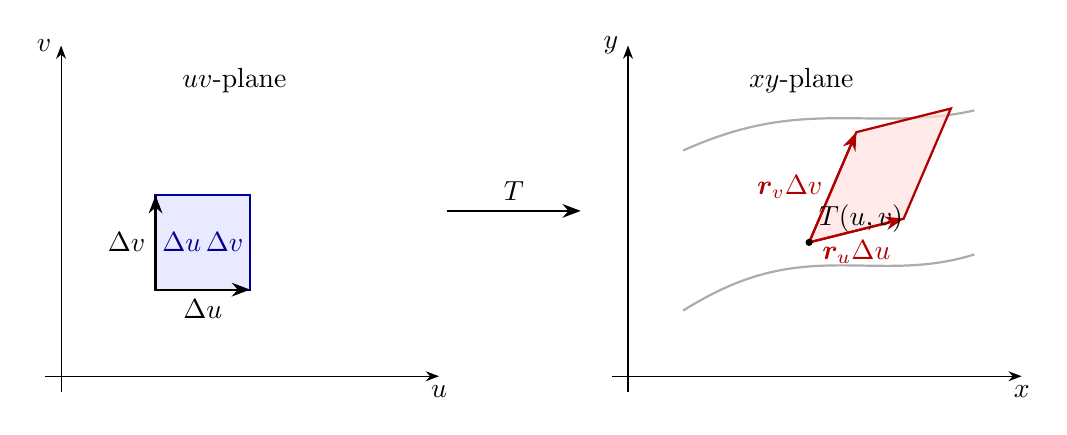
\begin{tikzpicture}[scale=1.0]
  % Left: uv-plane
  \begin{scope}
    \draw[-{Stealth}] (-0.2,0) -- (4.8,0) node[below] {$u$};
    \draw[-{Stealth}] (0,-0.2) -- (0,4.2) node[left] {$v$};

    % small rectangle in uv
    \fill[blue!12,opacity=0.7] (1.2,1.1) rectangle (2.4,2.3);
    \draw[blue!60!black,thick] (1.2,1.1) rectangle (2.4,2.3);
    \node[blue!60!black] at (1.8,1.7) {$\Delta u\,\Delta v$};

    % arrows showing basis directions
    \draw[-{Stealth},thick] (1.2,1.1) -- (2.4,1.1) node[midway,below] {$\Delta u$};
    \draw[-{Stealth},thick] (1.2,1.1) -- (1.2,2.3) node[midway,left] {$\Delta v$};

    \node at (2.2,3.75) {$uv$-plane};
  \end{scope}

  % Right: xy-plane (schematic)
  \begin{scope}[xshift=7.2cm]
    \draw[-{Stealth}] (-0.2,0) -- (5.0,0) node[below] {$x$};
    \draw[-{Stealth}] (0,-0.2) -- (0,4.2) node[left] {$y$};

    % draw a curved region boundary (schematic)
    \draw[gray!65,thick]
      plot[domain=0.7:4.4,samples=120] (\x,{0.6+0.35*(\x-0.7)+0.35*sin(60*\x)});
    \draw[gray!65,thick]
      plot[domain=0.7:4.4,samples=120] (\x,{2.7+0.25*(\x-0.7)+0.25*sin(60*\x)});

    % parallelogram image (local linearization)
    \coordinate (P) at (2.3,1.7);
    \coordinate (A) at (3.5,2.0);
    \coordinate (B) at (2.9,3.1);
    \coordinate (C) at (4.1,3.4);

    \fill[red!12,opacity=0.7] (P)--(A)--(C)--(B)--cycle;
    \draw[red!70!black,thick] (P)--(A)--(C)--(B)--cycle;

    \draw[-{Stealth},thick,red!70!black] (P)--(A) node[midway,below] {$\vect r_u\Delta u$};
    \draw[-{Stealth},thick,red!70!black] (P)--(B) node[midway,left] {$\vect r_v\Delta v$};

    \fill (P) circle (1.3pt);
    \node[above right] at (P) {$T(u,v)$};

    \node at (2.2,3.75) {$xy$-plane};
  \end{scope}

  % Arrow indicating mapping
  \draw[-{Stealth},thick] (4.9,2.1) -- (6.6,2.1) node[midway,above] {$T$};

\end{tikzpicture}
\caption{A small rectangle in the $uv$-plane maps to a small parallelogram in the $xy$-plane. The Jacobian gives the local area scaling.}
\label{fig:jacobian-geometry}
\end{figure}

\subsubsection{Properties of Jacobians}

\begin{proposition}[Jacobian of a linear map]\label{prop:linear-jac}
If
\[
x=au+bv,\qquad y=cu+dv,
\]
then
\[
\frac{\partial(x,y)}{\partial(u,v)}=
\begin{vmatrix}
a & b\\
c & d
\end{vmatrix}
=ad-bc.
\]
Geometrically, the unit square in $(u,v)$ maps to a parallelogram in $(x,y)$ with area $|ad-bc|$.
\end{proposition}

\begin{proposition}[Inverse function and reciprocal Jacobian]\label{prop:inverse-jac}
If $T$ is one-to-one and differentiable with differentiable inverse $T^{-1}$, and if
\[
J(u,v)=\frac{\partial(x,y)}{\partial(u,v)}\neq 0,
\]
then the Jacobian of the inverse satisfies
\begin{equation}\label{eq:inverse-jac}
\frac{\partial(u,v)}{\partial(x,y)}=\frac{1}{\frac{\partial(x,y)}{\partial(u,v)}}
\end{equation}
evaluated at corresponding points.
\end{proposition}

\begin{proposition}[Jacobian of a composition]\label{prop:comp-jac}
If $T:(u,v)\mapsto (x,y)$ and $S:(x,y)\mapsto (p,q)$ are differentiable, then
\[
\frac{\partial(p,q)}{\partial(u,v)}
=
\frac{\partial(p,q)}{\partial(x,y)}\,
\frac{\partial(x,y)}{\partial(u,v)}.
\]
\end{proposition}

\begin{exercise}
Let $T(u,v)=(x,y)=(u+2v,\,3u-v)$.
\begin{enumerate}[label=(\alph*)]
\item Compute $\dfrac{\partial(x,y)}{\partial(u,v)}$.
\item Find the area of the image of the rectangle $0\le u\le 2$, $0\le v\le 1$ under $T$.
\end{enumerate}
\end{exercise}

% -------------------------------------------------
\subsection{Lesson 6.2: Double Integrals in General Coordinates}

\subsubsection{Change of Variables Theorem (Double Integrals)}

\begin{theorem}[Change of variables in $\RR^2$]\label{thm:cov2}
Let $T:(u,v)\mapsto (x,y)$ be a one-to-one $C^1$ transformation mapping a region $D^\ast$ in the $uv$-plane onto a region $D$ in the $xy$-plane. Assume the Jacobian
\[
J(u,v)=\frac{\partial(x,y)}{\partial(u,v)}
\]
is continuous and nonzero on $D^\ast$. If $f$ is continuous on $D$, then
\begin{equation}\label{eq:cov2}
\iint_D f(x,y)\,dA
=
\iint_{D^\ast} f(x(u,v),y(u,v))\,\left|J(u,v)\right|\,du\,dv.
\end{equation}
\end{theorem}

\begin{remark}[What the formula is saying]
Replace $(x,y)$ by your formulas in terms of $(u,v)$, and multiply by the scale factor $\left|J\right|$.  
The absolute value is essential: even if the mapping flips orientation (negative Jacobian), physical area must remain positive.
\end{remark}

\subsubsection{Transforming Regions}

\begin{definition}[Image and preimage]
If $D^\ast$ is a region in the $uv$-plane, its image is $D=T(D^\ast)$ in the $xy$-plane.  
Conversely, if $D$ is described naturally in $xy$, you try to find a transformation so that $D^\ast=T^{-1}(D)$ has simpler bounds.
\end{definition}

\begin{example}[Area of an ellipse via a scaling map]\label{ex:ellipse-area}
Let
\[
D=\left\{(x,y):\frac{x^2}{a^2}+\frac{y^2}{b^2}\le 1\right\},\qquad a>0,\ b>0.
\]
Use the substitution $x=au$, $y=bv$. Then
\[
\frac{x^2}{a^2}+\frac{y^2}{b^2}=u^2+v^2,
\]
so $D^\ast$ is the unit disk $u^2+v^2\le 1$. The Jacobian is
\[
\frac{\partial(x,y)}{\partial(u,v)}=
\begin{vmatrix}
a & 0\\
0 & b
\end{vmatrix}
=ab.
\]
Therefore,
\[
\operatorname{Area}(D)=\iint_D 1\,dA
=\iint_{D^\ast} 1\cdot |ab|\,du\,dv
=ab\cdot \operatorname{Area}(D^\ast)
=ab\cdot \pi
=\pi ab.
\]
\end{example}

\begin{example}[A Gaussian-shaped integral on an ellipse]\label{ex:ellipse-gaussian}
Let $D$ be the ellipse in \cref{ex:ellipse-area} and consider
\[
I=\iint_D \exp\!\left(-\frac{x^2}{a^2}-\frac{y^2}{b^2}\right)\,dA.
\]
With $x=au$, $y=bv$, we have $\exp(-(x^2/a^2)-(y^2/b^2))=\exp(-(u^2+v^2))$ and $dA=|ab|\,du\,dv=ab\,du\,dv$. Hence
\[
I=ab\iint_{u^2+v^2\le 1} e^{-(u^2+v^2)}\,du\,dv.
\]
At this stage, switching to polar in the $uv$-plane finishes it:
\[
I=ab\int_{0}^{2\pi}\int_{0}^{1} e^{-r^2}\,r\,dr\,d\theta
=ab\cdot 2\pi \cdot \left[-\frac12 e^{-r^2}\right]_{0}^{1}
=ab\pi\,(1-e^{-1}).
\]
\end{example}

\subsubsection{Polar Coordinates as a Special Case}

\begin{proposition}[Polar Jacobian]\label{prop:polar-jac}
Let
\[
x=r\cos\theta,\qquad y=r\sin\theta,\qquad r\ge 0.
\]
Then
\[
\frac{\partial(x,y)}{\partial(r,\theta)}
=
\begin{vmatrix}
\cos\theta & -r\sin\theta\\
\sin\theta & r\cos\theta
\end{vmatrix}
=r(\cos^2\theta+\sin^2\theta)=r,
\]
so
\begin{equation}\label{eq:polar-area-element}
dA=r\,dr\,d\theta.
\end{equation}
\end{proposition}

\begin{remark}[Practical cue]
If you see circles, disks, annuli, or expressions like $x^2+y^2$, polar coordinates are usually the right tool because they turn $x^2+y^2$ into $r^2$ and simplify the region.
\end{remark}

\begin{exercise}
Evaluate
\[
\iint_D (x^2+y^2)\,dA
\quad\text{where}\quad
D=\{(x,y):1\le x^2+y^2\le 4\}.
\]
Use polar coordinates and show each bound clearly.
\end{exercise}

% -------------------------------------------------
\subsection{Lesson 6.3: Cylindrical and Spherical Coordinates}

\subsubsection{Cylindrical Coordinates}

\begin{definition}[Cylindrical coordinates]\label{def:cyl}
Cylindrical coordinates represent points in $\RR^3$ by $(r,\theta,z)$:
\[
x=r\cos\theta,\qquad y=r\sin\theta,\qquad z=z,
\]
with $r\ge 0$ and $\theta$ measured in the $xy$-plane.
\end{definition}

\begin{proposition}[Volume element in cylindrical coordinates]\label{prop:cyl-vol}
Under $(x,y,z)=(r\cos\theta,r\sin\theta,z)$, the Jacobian determinant is $r$, so
\begin{equation}\label{eq:cyl-dV}
dV=r\,dr\,d\theta\,dz.
\end{equation}
\end{proposition}

\begin{example}[Volume of a right circular cylinder]
Let $E=\{(x,y,z):x^2+y^2\le a^2,\ 0\le z\le h\}$. In cylindrical coordinates:
\[
0\le r\le a,\qquad 0\le \theta\le 2\pi,\qquad 0\le z\le h.
\]
Thus
\[
\operatorname{Vol}(E)=\iiint_E 1\,dV
=\int_{0}^{h}\int_{0}^{2\pi}\int_{0}^{a} 1\cdot r\,dr\,d\theta\,dz
=\int_{0}^{h}\left(2\pi\cdot \frac{a^2}{2}\right)dz
=\pi a^2 h.
\]
\end{example}

\subsubsection{Spherical Coordinates}

\begin{definition}[Spherical coordinates]\label{def:sph}
Spherical coordinates represent points in $\RR^3$ by $(\rho,\phi,\theta)$:
\[
x=\rho\sin\phi\cos\theta,\qquad
y=\rho\sin\phi\sin\theta,\qquad
z=\rho\cos\phi,
\]
where $\rho\ge 0$ is distance from the origin, $0\le \phi\le \pi$ is the angle from the positive $z$-axis (polar angle), and $0\le \theta\le 2\pi$ is the angle in the $xy$-plane (azimuth).
\end{definition}

\begin{proposition}[Volume element in spherical coordinates]\label{prop:sph-vol}
Under $(x,y,z)=(\rho\sin\phi\cos\theta,\allowbreak \rho\sin\phi\sin\theta,\allowbreak \rho\cos\phi)$, the Jacobian determinant is $\rho^2\sin\phi$, so
\begin{equation}\label{eq:sph-dV}
dV=\rho^2\sin\phi\,d\rho\,d\phi\,d\theta.
\end{equation}
\end{proposition}

\begin{remark}[Memory aid]
In spherical, the volume scale has two effects:
\begin{itemize}
\item $\rho^2$ because spheres grow like “radius squared” in surface area,
\item $\sin\phi$ because slices at polar angle $\phi$ have radius $\rho\sin\phi$ in the $xy$-direction.
\end{itemize}
\end{remark}

\begin{figure}[H]
\centering
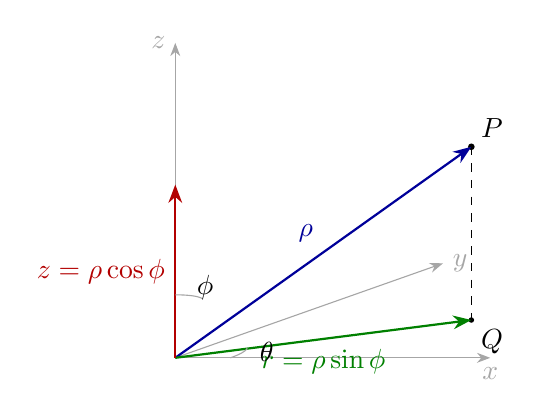
\begin{tikzpicture}[scale=1.0,
  x={(1.0cm,0.0cm)},
  y={(0.85cm,0.30cm)},
  z={(0.0cm,1.0cm)}]

  % axes
  \draw[-{Stealth},gray!70] (0,0,0) -- (4.0,0,0) node[below] {$x$};
  \draw[-{Stealth},gray!70] (0,0,0) -- (0,4.0,0) node[right] {$y$};
  \draw[-{Stealth},gray!70] (0,0,0) -- (0,0,4.0) node[left] {$z$};

  % point in space (schematic)
  \coordinate (O) at (0,0,0);
  \coordinate (P) at (2.4,1.6,2.2);
  \fill (P) circle (1.2pt);
  \node[above right] at (P) {$P$};

  % radial vector rho
  \draw[-{Stealth},thick,blue!60!black] (O) -- (P) node[midway,above left] {$\rho$};

  % projection onto xy-plane
  \coordinate (Q) at (2.4,1.6,0);
  \draw[dashed] (P) -- (Q);
  \fill (Q) circle (1.0pt);
  \node[below right] at (Q) {$Q$};

  % r in cylindrical sense
  \draw[-{Stealth},thick,green!50!black] (O) -- (Q) node[midway,below] {$r=\rho\sin\phi$};

  % show z component
  \draw[-{Stealth},thick,red!70!black] (O) -- (0,0,2.2) node[midway,left] {$z=\rho\cos\phi$};

  % small arc for theta in xy-plane (schematic)
  \draw[gray!70] (0.7,0,0) arc[start angle=0,end angle=35,radius=0.7];
  \node at (0.95,0.25,0) {$\theta$};

  % indicate phi (schematic arc in plane containing z-axis and OP)
  % draw a short arc near origin in that plane (approx)
  \draw[gray!70] (0,0,0.8) arc[start angle=90,end angle=52,radius=0.8];
  \node at (0.25,0.15,0.85) {$\phi$};

\end{tikzpicture}
\caption{Cylindrical and spherical geometry: $r$ is the projection radius in the $xy$-plane, while $\rho$ is the full distance to the origin. Angles $\theta$ (azimuth) and $\phi$ (polar angle) locate direction.}
\label{fig:cyl-sph}
\end{figure}

\subsubsection{Applications to Triple Integrals}

\begin{theorem}[Triple integrals in cylindrical coordinates]\label{thm:triple-cyl}
If a solid $E$ is described by bounds in $(r,\theta,z)$, then
\[
\iiint_E F(x,y,z)\,dV
=
\iiint_{E^\ast} F(r\cos\theta,r\sin\theta,z)\, r\,dr\,d\theta\,dz,
\]
with the bounds taken over the corresponding region $E^\ast$ in $(r,\theta,z)$-space.
\end{theorem}

\begin{theorem}[Triple integrals in spherical coordinates]\label{thm:triple-sph}
If a solid $E$ is described by bounds in $(\rho,\phi,\theta)$, then
\[
\iiint_E F(x,y,z)\,dV
=
\iiint_{E^\ast} F(\rho\sin\phi\cos\theta,\rho\sin\phi\sin\theta,\rho\cos\phi)\,
\rho^2\sin\phi\,d\rho\,d\phi\,d\theta.
\]
\end{theorem}

\begin{example}[Volume of a ball]\label{ex:ball-volume}
Compute the volume of the ball $\rho\le a$ (i.e.\ $x^2+y^2+z^2\le a^2$).
In spherical coordinates:
\[
0\le \rho\le a,\qquad 0\le \phi\le \pi,\qquad 0\le \theta\le 2\pi.
\]
Thus
\[
\operatorname{Vol}=\iiint_E 1\,dV
=\int_{0}^{2\pi}\int_{0}^{\pi}\int_{0}^{a} 1\cdot \rho^2\sin\phi\,d\rho\,d\phi\,d\theta
=\left(\int_{0}^{2\pi}d\theta\right)\left(\int_{0}^{\pi}\sin\phi\,d\phi\right)\left(\int_{0}^{a}\rho^2\,d\rho\right).
\]
Compute each factor:
\[
\int_{0}^{2\pi}d\theta=2\pi,\qquad
\int_{0}^{\pi}\sin\phi\,d\phi=\big[-\cos\phi\big]_{0}^{\pi}=2,\qquad
\int_{0}^{a}\rho^2\,d\rho=\frac{a^3}{3}.
\]
Therefore $\operatorname{Vol}=\dfrac{4}{3}\pi a^3$.
\end{example}

\begin{example}[A symmetric integral over a ball]
Evaluate
\[
I=\iiint_{x^2+y^2+z^2\le a^2} (x^2+y^2+z^2)\,dV.
\]
In spherical, $x^2+y^2+z^2=\rho^2$, so
\[
I=\int_{0}^{2\pi}\int_{0}^{\pi}\int_{0}^{a} \rho^2\cdot \rho^2\sin\phi\,d\rho\,d\phi\,d\theta
=\left(\int_{0}^{2\pi}d\theta\right)\left(\int_{0}^{\pi}\sin\phi\,d\phi\right)\left(\int_{0}^{a}\rho^4\,d\rho\right)
=2\pi\cdot 2\cdot \frac{a^5}{5}
=\frac{4\pi}{5}a^5.
\]
\end{example}

\begin{exercise}
Set up (and evaluate) the integral for the volume inside the paraboloid $z=4-r^2$ and above the plane $z=0$ using cylindrical coordinates.
\end{exercise}

\begin{exercise}
Use spherical coordinates to compute the mass of the solid ball $x^2+y^2+z^2\le a^2$ with density $\rho(x,y,z)=k\sqrt{x^2+y^2+z^2}$, where $k>0$ is constant.
\end{exercise}

\subsubsection*{Chapter 6 Checklist}
\begin{itemize}
\item The Jacobian $\dfrac{\partial(x,y)}{\partial(u,v)}=x_u y_v-x_v y_u$ is the local area scale factor.
\item Change of variables for double integrals:
\[
\iint_D f(x,y)\,dA=\iint_{D^\ast} f(x(u,v),y(u,v))\left|\frac{\partial(x,y)}{\partial(u,v)}\right|\,du\,dv.
\]
\item Polar is a special case: $dA=r\,dr\,d\theta$.
\item Cylindrical coordinates: $dV=r\,dr\,d\theta\,dz$.
\item Spherical coordinates: $dV=\rho^2\sin\phi\,d\rho\,d\phi\,d\theta$.
\end{itemize}

% =========================
% End of Chapter 6
% =========================

% =========================
% Chapter 7 (no preamble)
% =========================

\section{Chapter 7: Vector Calculus}

\begin{keyidea}
Vector calculus connects geometry, differentiation, and integration in a powerful way.

\begin{itemize}
\item A \emph{vector field} assigns a vector to each point in space (think: wind velocity, fluid flow, force).
\item \emph{Line integrals} measure accumulated work or circulation along a curve.
\item \emph{Flux integrals} measure flow through a curve/surface.
\item The big theorems (Green, Stokes, Divergence) convert hard integrals into easier ones by swapping “boundary” and “interior.”
\end{itemize}
\end{keyidea}

% -------------------------------------------------
\subsection{Lesson 7.1: Vector Fields}

\subsubsection{Definitions and Examples}

\begin{definition}[Vector field]
A \emph{vector field} on a region $D\subset\RR^n$ is a function
\[
\vect F:D\to\RR^n,\qquad \vect F(\vect x)=\langle F_1(\vect x),\dots,F_n(\vect x)\rangle.
\]
In $\RR^2$, write $\vect F(x,y)=\langle P(x,y),Q(x,y)\rangle$.  
In $\RR^3$, write $\vect F(x,y,z)=\langle P(x,y,z),Q(x,y,z),R(x,y,z)\rangle$.
\end{definition}

\begin{example}[Typical fields]
\begin{enumerate}[label=(\alph*)]
\item Radial field in $\RR^2$: $\vect F(x,y)=\langle x,y\rangle$ (points away from the origin).
\item Rotational field in $\RR^2$: $\vect F(x,y)=\langle -y,x\rangle$ (circles around the origin).
\item Inverse-square-type (away from origin) in $\RR^3$: $\vect F=\dfrac{1}{(x^2+y^2+z^2)^{3/2}}\langle x,y,z\rangle$.
\end{enumerate}
\end{example}

\begin{remark}[Physical intuition]
A vector field is a “vector at every point.” If it is velocity, field lines show how a particle would flow; if it is force, field lines show force directions.
\end{remark}

\subsubsection{Gradient Fields and Potential Functions}

\begin{definition}[Gradient field / conservative field]\label{def:conservative}
A vector field $\vect F$ on a region $D\subset\RR^n$ is \emph{conservative} (or a \emph{gradient field}) if there exists a scalar function $f$ such that
\[
\vect F=\nabla f.
\]
The function $f$ is called a \emph{potential function} for $\vect F$.
\end{definition}

\begin{example}[A gradient field]
Let $f(x,y)=x^2y+y^3$. Then
\[
\nabla f=\langle 2xy,\ x^2+3y^2\rangle.
\]
So $\vect F(x,y)=\langle 2xy,\ x^2+3y^2\rangle$ is conservative on $\RR^2$.
\end{example}

\subsubsection{Visualizing Vector Fields (Sketching)}

\begin{figure}[H]
\centering
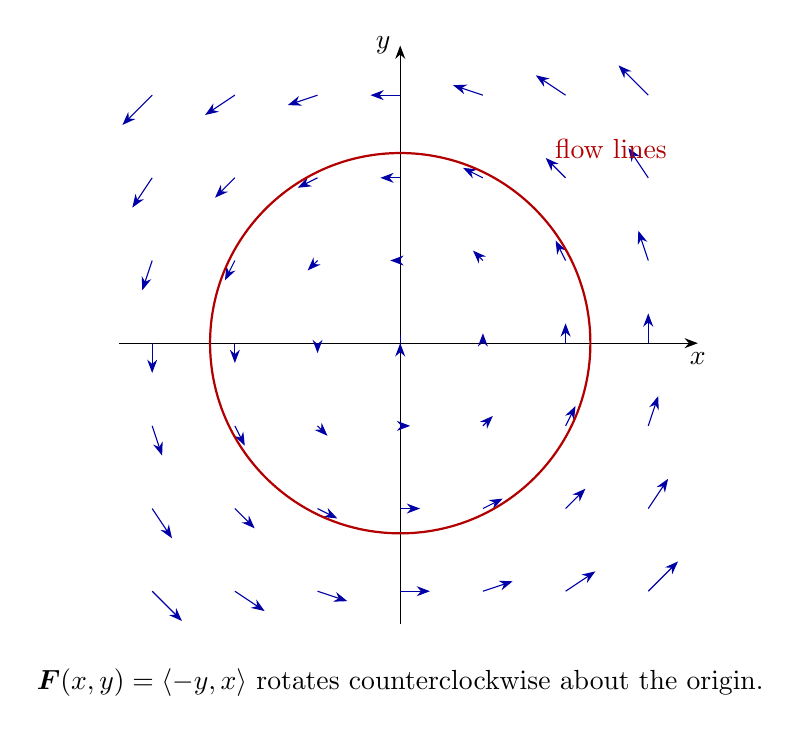
\begin{tikzpicture}[scale=1.05]
  % axes
  \draw[-{Stealth}] (-3.4,0) -- (3.6,0) node[below] {$x$};
  \draw[-{Stealth}] (0,-3.4) -- (0,3.6) node[left] {$y$};

  % field F(x,y) = <-y, x> on a grid (rotational)
  \foreach \i in {-3,-2,...,3} {
    \foreach \j in {-3,-2,...,3} {
      \pgfmathsetmacro{\vx}{-(\j)}   % -y
      \pgfmathsetmacro{\vy}{(\i)}    % x
      % scale down arrows
      \pgfmathsetmacro{\sx}{0.12*\vx}
      \pgfmathsetmacro{\sy}{0.12*\vy}
      \draw[-{Stealth},blue!65!black] (\i,\j) -- (\i+\sx,\j+\sy);
    }
  }

  % circle to suggest flow
  \draw[red!70!black,thick] (0,0) circle (2.3);
  \node[red!70!black] at (2.55,2.35) {flow lines};

  \node at (0,-4.1) {$\vect F(x,y)=\langle -y,x\rangle$ rotates counterclockwise about the origin.};
\end{tikzpicture}
\caption{A rotational vector field in $\RR^2$: arrows circulate around the origin.}
\label{fig:vectorfield-rot}
\end{figure}

\begin{exercise}
For $\vect F(x,y)=\langle x, -y\rangle$, describe qualitatively how the arrows point in each quadrant. Is the field more like “source/sink” or “rotation”?
\end{exercise}

% -------------------------------------------------
\subsection{Lesson 7.2: Line Integrals}

\subsubsection{Line Integrals of Scalar Functions}

\begin{definition}[Line integral of a scalar function]\label{def:line-scalar}
Let $C$ be a smooth curve parametrized by $\vect r(t)$, $a\le t\le b$, and let $f$ be continuous on $C$. Then
\begin{equation}\label{eq:line-scalar}
\int_C f\,ds = \int_a^b f(\vect r(t))\,\norm{\vect r'(t)}\,dt.
\end{equation}
\end{definition}

\begin{remark}[Interpretation]
$\int_C f\,ds$ adds up $f$ weighted by arc length. For example, if $f$ is density along a wire, then $\int_C f\,ds$ is total mass.
\end{remark}

\subsubsection{Line Integrals of Vector Fields (Work Integrals)}

\begin{definition}[Work / circulation line integral]\label{def:line-work}
Let $\vect F$ be a vector field and $C$ be a smooth curve oriented by $\vect r(t)$, $a\le t\le b$. Then
\begin{equation}\label{eq:line-work}
\int_C \vect F\cdot d\vect r
=
\int_a^b \vect F(\vect r(t))\cdot \vect r'(t)\,dt.
\end{equation}
\end{definition}

\begin{remark}[Physics meaning]
If $\vect F$ is force and $\vect r(t)$ is a path, then $\int_C \vect F\cdot d\vect r$ is the work done by the force along that path.
\end{remark}

\subsubsection{Basic Parametrization Examples}

\begin{example}[Scalar line integral on a circle]
Let $C$ be the circle $x^2+y^2=4$ traversed once counterclockwise. Parameterize:
\[
\vect r(t)=\langle 2\cos t,\ 2\sin t\rangle,\qquad 0\le t\le 2\pi.
\]
Then $\norm{\vect r'(t)}=\norm{\langle -2\sin t,\ 2\cos t\rangle}=2$.  
For $f(x,y)=x^2+y^2$, we have $f(\vect r(t))=4$. Hence
\[
\int_C f\,ds=\int_0^{2\pi} 4\cdot 2\,dt = 16\pi.
\]
\end{example}

\begin{example}[Work integral]\label{ex:work}
Let $\vect F(x,y)=\langle -y,x\rangle$ and let $C$ be the unit circle $x^2+y^2=1$ counterclockwise.  
Use $\vect r(t)=\langle \cos t,\sin t\rangle$, $0\le t\le 2\pi$.
Then
\[
\vect r'(t)=\langle -\sin t,\ \cos t\rangle,\qquad
\vect F(\vect r(t))=\langle -\sin t,\ \cos t\rangle.
\]
So
\[
\vect F(\vect r(t))\cdot \vect r'(t)
=\langle -\sin t,\cos t\rangle\cdot \langle -\sin t,\cos t\rangle
=\sin^2 t+\cos^2 t=1.
\]
Therefore
\[
\int_C \vect F\cdot d\vect r=\int_{0}^{2\pi}1\,dt=2\pi.
\]
\end{example}

\begin{exercise}
Compute $\displaystyle \int_C (x+y)\,ds$ where $C$ is the line segment from $(0,0)$ to $(2,1)$.
(Hint: parametrize $\vect r(t)=\langle 2t,t\rangle$, $0\le t\le 1$.)
\end{exercise}

% -------------------------------------------------
\subsection{Lesson 7.3: The Fundamental Theorem for Line Integrals}

\subsubsection{Path Independence and Conservative Fields}

\begin{theorem}[Fundamental Theorem for Line Integrals]\label{thm:ftli}
Let $\vect F=\nabla f$ be a conservative vector field on a region $D$, and let $C$ be a smooth curve in $D$ from point $A$ to point $B$. Then
\begin{equation}\label{eq:ftli}
\int_C \vect F\cdot d\vect r = f(B)-f(A).
\end{equation}
In particular, the integral depends only on endpoints, not on the path.
\end{theorem}

\begin{corollary}[Zero circulation on closed curves]\label{cor:closed-zero}
If $\vect F=\nabla f$ and $C$ is a closed curve (start = end), then
\[
\oint_C \vect F\cdot d\vect r = 0.
\]
\end{corollary}

\begin{remark}[How to use it]
If you can find a potential function $f$, you avoid parametrizing curves entirely: compute $f(B)-f(A)$ and you are done.
\end{remark}

\subsubsection{Characterizing Conservative Fields in $\RR^2$}

\begin{theorem}[Curl test in $\RR^2$ (simply connected domains)]\label{thm:conservative-test}
Let $\vect F(x,y)=\langle P(x,y),Q(x,y)\rangle$ with continuous partial derivatives on a simply connected region $D\subset\RR^2$.  
Then $\vect F$ is conservative on $D$ if and only if
\begin{equation}\label{eq:curl2}
\frac{\partial P}{\partial y}=\frac{\partial Q}{\partial x}\quad \text{everywhere on }D.
\end{equation}
\end{theorem}

\begin{remark}[Why “simply connected” matters]
If the region has holes, a field can satisfy $\partial P/\partial y=\partial Q/\partial x$ and still fail to be globally conservative.  
Example: $\langle -y/(x^2+y^2),\ x/(x^2+y^2)\rangle$ on $\RR^2\setminus\{(0,0)\}$ has nontrivial circulation around the origin.
\end{remark}

\subsubsection{Finding a Potential Function}

\begin{proposition}[How to find $f$ when $\vect F=\langle P,Q\rangle$ is conservative]\label{prop:find-potential}
Assume $f_x=P$ and $f_y=Q$.
\begin{enumerate}[label=(\arabic*)]
\item Integrate $P$ with respect to $x$ to get $f(x,y)=\int P(x,y)\,dx + g(y)$.
\item Differentiate this expression with respect to $y$ and set it equal to $Q$ to determine $g'(y)$.
\item Integrate $g'(y)$ to get $g(y)$ and complete $f$ (up to an additive constant).
\end{enumerate}
\end{proposition}

\begin{example}[Using the FTLI]
Let $\vect F(x,y)=\langle 2xy,\ x^2+3y^2\rangle$. We claim $\vect F$ is conservative on $\RR^2$.
Check:
\[
\frac{\partial P}{\partial y}=2x,\qquad \frac{\partial Q}{\partial x}=2x,
\]
so \cref{eq:curl2} holds and $D=\RR^2$ is simply connected.

Find a potential $f$:
\[
f_x=2xy \implies f(x,y)=\int 2xy\,dx=x^2y+g(y).
\]
Differentiate:
\[
f_y=x^2+g'(y).
\]
Set $f_y=Q=x^2+3y^2$ gives $g'(y)=3y^2$, so $g(y)=y^3$. Thus
\[
f(x,y)=x^2y+y^3.
\]

Now compute the work from $A=(0,1)$ to $B=(2,0)$ along any path:
\[
\int_C \vect F\cdot d\vect r=f(B)-f(A)=\big(2^2\cdot 0+0^3\big)-\big(0^2\cdot 1+1^3\big)=0-1=-1.
\]
\end{example}

\begin{exercise}
Determine whether $\vect F(x,y)=\langle y\cos x,\ \sin x\rangle$ is conservative on $\RR^2$.
If it is, find a potential $f$ and compute $\int_C \vect F\cdot d\vect r$ from $(0,0)$ to $(\pi,1)$.
\end{exercise}

% -------------------------------------------------
\subsection{Lesson 7.4: Green's Theorem}

\subsubsection{Circulation Form of Green's Theorem}

\begin{theorem}[Green's Theorem (circulation form)]\label{thm:green}
Let $C$ be a positively oriented (counterclockwise), simple, closed, piecewise-smooth curve in the plane, and let $D$ be the region it encloses.  
If $\vect F=\langle P,Q\rangle$ has continuous partial derivatives on an open region containing $D$, then
\begin{equation}\label{eq:green-circ}
\oint_C P\,dx+Q\,dy
=
\iint_D \left(\frac{\partial Q}{\partial x}-\frac{\partial P}{\partial y}\right)\,dA.
\end{equation}
\end{theorem}

\begin{remark}[What it does]
A line integral around the boundary becomes a double integral over the interior.  
This is usually a huge simplification when the boundary is complicated but the interior is easy (or vice versa).
\end{remark}

\subsubsection{Flux Form of Green's Theorem}

\begin{definition}[Outward unit normal in the plane]
If $C$ is oriented counterclockwise with tangent direction $d\vect r=\langle dx,dy\rangle$, then an outward normal line element can be represented by
\[
\vect n\,ds=\langle dy,\ -dx\rangle.
\]
\end{definition}

\begin{theorem}[Green's Theorem (flux form)]\label{thm:green-flux}
With the same hypotheses as \cref{thm:green}, we have
\begin{equation}\label{eq:green-flux}
\oint_C \vect F\cdot \vect n\,ds
=
\oint_C P\,dy - Q\,dx
=
\iint_D \left(\frac{\partial P}{\partial x}+\frac{\partial Q}{\partial y}\right)\,dA.
\end{equation}
\end{theorem}

\begin{remark}[Divergence in 2D]
The integrand $\dfrac{\partial P}{\partial x}+\dfrac{\partial Q}{\partial y}$ is the \emph{2D divergence}. The flux form says: total outward flux through the boundary equals the integral of divergence over the region.
\end{remark}

\subsubsection{Applications}

\begin{example}[Compute area using Green's Theorem]\label{ex:area-green}
Take $P=-\dfrac{y}{2}$ and $Q=\dfrac{x}{2}$. Then
\[
\frac{\partial Q}{\partial x}-\frac{\partial P}{\partial y}
=\frac12-\left(-\frac12\right)=1.
\]
By \cref{eq:green-circ},
\[
\oint_C \left(-\frac{y}{2}\,dx+\frac{x}{2}\,dy\right)
=\iint_D 1\,dA=\operatorname{Area}(D).
\]
So
\begin{equation}\label{eq:area-formula}
\operatorname{Area}(D)=\frac12\oint_C (x\,dy-y\,dx).
\end{equation}
\end{example}

\begin{example}[Work around a circle quickly]
Let $\vect F=\langle -y,x\rangle$ and let $C$ be the unit circle oriented counterclockwise. In \cref{ex:work} we computed the circulation as $2\pi$ by parametrization.  
Now use Green:
\[
\frac{\partial Q}{\partial x}-\frac{\partial P}{\partial y}
=\frac{\partial}{\partial x}(x)-\frac{\partial}{\partial y}(-y)=1-(-1)=2.
\]
Hence
\[
\oint_C P\,dx+Q\,dy=\iint_D 2\,dA=2\cdot \operatorname{Area}(\text{unit disk})=2\cdot \pi=2\pi,
\]
agreeing with the earlier result.
\end{example}

\begin{figure}[H]
\centering
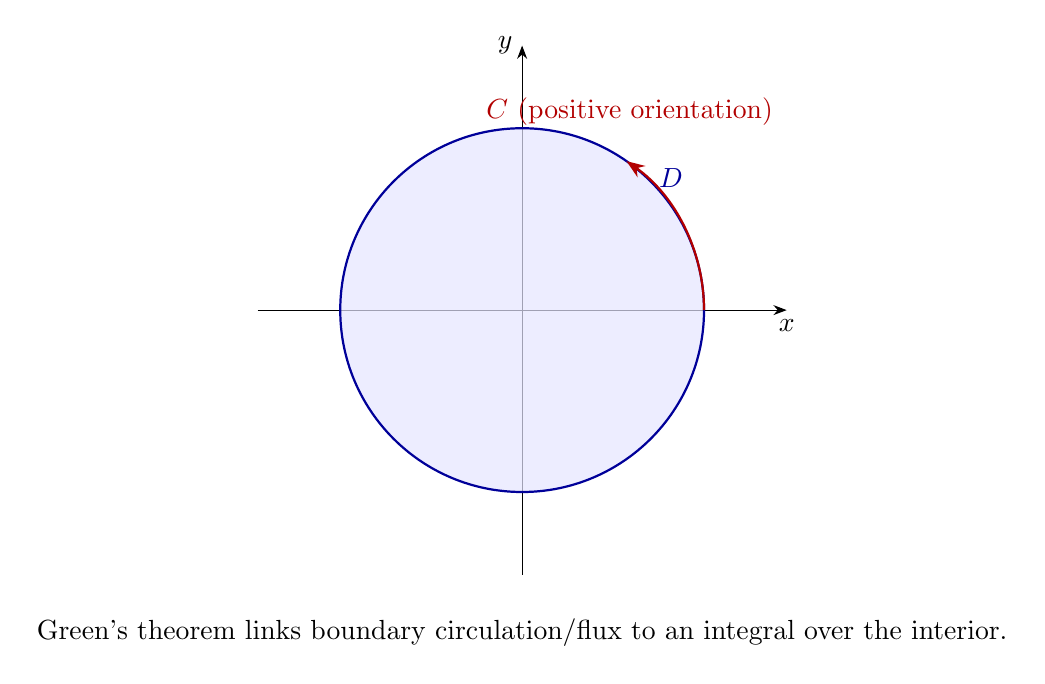
\begin{tikzpicture}[scale=1.05]
  \draw[-{Stealth}] (-3.2,0) -- (3.2,0) node[below] {$x$};
  \draw[-{Stealth}] (0,-3.2) -- (0,3.2) node[left] {$y$};

  % region D: unit disk
  \fill[blue!10,opacity=0.7] (0,0) circle (2.2);
  \draw[blue!60!black,thick] (0,0) circle (2.2);
  \node[blue!60!black] at (1.8,1.6) {$D$};

  % boundary C arrow (counterclockwise)
  \draw[-{Stealth},red!70!black,thick] (2.2,0) arc[start angle=0,end angle=55,radius=2.2];
  \node[red!70!black] at (1.3,2.4) {$C$ (positive orientation)};

  \node at (0,-3.9) {Green's theorem links boundary circulation/flux to an integral over the interior.};
\end{tikzpicture}
\caption{A positively oriented boundary curve $C$ enclosing a region $D$.}
\label{fig:green-setup}
\end{figure}

\begin{exercise}
Use Green's Theorem to compute
\[
\oint_C (x^2-y^2)\,dx + 2xy\,dy
\]
where $C$ is the positively oriented circle $x^2+y^2=1$.
\end{exercise}

% -------------------------------------------------
\subsection{Lesson 7.5: Curl and Divergence}

\subsubsection{Definitions in $\RR^3$}

\begin{definition}[Divergence]\label{def:div}
For a $C^1$ vector field $\vect F=\langle P,Q,R\rangle$ on $\RR^3$, the divergence is
\[
\nabla\cdot \vect F = P_x+Q_y+R_z.
\]
\end{definition}

\begin{definition}[Curl]\label{def:curl}
For a $C^1$ vector field $\vect F=\langle P,Q,R\rangle$ on $\RR^3$, the curl is
\[
\nabla\times \vect F
=
\left\langle
R_y-Q_z,\ 
P_z-R_x,\ 
Q_x-P_y
\right\rangle.
\]
\end{definition}

\begin{remark}[Interpretation]
Divergence measures “net outflow per unit volume” (sources/sinks).  
Curl measures “local rotation” (circulation density).
\end{remark}

\subsubsection{Key Identities}

\begin{proposition}[Always true identities]\label{prop:identities}
If $f$ is $C^2$ and $\vect F$ is $C^2$, then
\[
\nabla\times(\nabla f)=\vect 0,
\qquad
\nabla\cdot(\nabla\times \vect F)=0.
\]
\end{proposition}

\begin{remark}[A practical consequence]
If $\vect F$ is a gradient field ($\vect F=\nabla f$), then $\nabla\times \vect F=\vect 0$.  
This is a necessary condition for being conservative; in simply connected regions it is also sufficient.
\end{remark}

\subsubsection{Examples}

\begin{example}[Compute divergence and curl]
Let $\vect F(x,y,z)=\langle x^2y,\ yz,\ xz^2\rangle$.
Then
\[
\nabla\cdot \vect F
=\frac{\partial}{\partial x}(x^2y)+\frac{\partial}{\partial y}(yz)+\frac{\partial}{\partial z}(xz^2)
=2xy+z+2xz.
\]
Also
\begin{align*}
\nabla\times \vect F
&= \left\langle R_y-Q_z,\ P_z-R_x,\ Q_x-P_y \right\rangle \\[8pt]
&= \begin{bmatrix}
\dfrac{\partial}{\partial y}(xz^2)-\dfrac{\partial}{\partial z}(yz) \\[8pt]
\dfrac{\partial}{\partial z}(x^2y)-\dfrac{\partial}{\partial x}(xz^2) \\[8pt]
\dfrac{\partial}{\partial x}(yz)-\dfrac{\partial}{\partial y}(x^2y)
\end{bmatrix}^T \\[8pt]
&= \langle 0-y,\ 0-z^2,\ 0-x^2 \rangle \\[5pt]
&= \langle -y,\ -z^2,\ -x^2\rangle.
\end{align*}
\end{example}

\begin{exercise}
Let $\vect F=\langle yz,\ xz,\ xy\rangle$.
\begin{enumerate}[label=(\alph*)]
\item Compute $\nabla\cdot \vect F$.
\item Compute $\nabla\times \vect F$.
\item Is $\vect F$ conservative on $\RR^3$? (Justify.)
\end{enumerate}
\end{exercise}

% -------------------------------------------------
\subsection{Lesson 7.6: Stokes' Theorem and the Divergence Theorem}

\subsubsection{Stokes' Theorem}

\begin{theorem}[Stokes' Theorem]\label{thm:stokes}
Let $S$ be an oriented, smooth surface with boundary curve $\partial S=C$ (a closed curve).
Let $\vect n$ be the unit normal consistent with the positive orientation of $C$ (right-hand rule).
If $\vect F$ has continuous partial derivatives on an open region containing $S$, then
\begin{equation}\label{eq:stokes}
\oint_{C} \vect F\cdot d\vect r
=
\iint_{S} (\nabla\times \vect F)\cdot \vect n\,dS.
\end{equation}
\end{theorem}

\begin{remark}[Meaning]
A circulation integral around the boundary equals the flux of curl through the surface.  
It is the 3D analogue of Green's theorem.
\end{remark}

\begin{example}[A simple Stokes computation: choose the easiest surface]\label{ex:stokes-disk}
Let $\vect F=\langle -y,x,0\rangle$ and let $C$ be the circle $x^2+y^2=1$ in the plane $z=0$ oriented counterclockwise (viewed from $+z$).
Choose $S$ to be the unit disk in the plane $z=0$ with upward normal $\vect n=\langle 0,0,1\rangle$.

Compute curl:
\[
\nabla\times \vect F
=
\left\langle
0-0,\ 0-0,\ \frac{\partial}{\partial x}(x)-\frac{\partial}{\partial y}(-y)
\right\rangle
=
\langle 0,0,2\rangle.
\]
Then
\[
\iint_S (\nabla\times \vect F)\cdot \vect n\,dS
=
\iint_S 2\,dS
=2\cdot \operatorname{Area}(\text{unit disk})
=2\pi.
\]
Hence, by Stokes,
\[
\oint_C \vect F\cdot d\vect r =2\pi,
\]
matching Chapter 7 line-integral computations.
\end{example}

\subsubsection{Divergence Theorem}

\begin{theorem}[Divergence Theorem (Gauss)]\label{thm:divthm}
Let $E$ be a solid region in $\RR^3$ with closed, piecewise-smooth boundary surface $S=\partial E$ oriented outward.
If $\vect F$ has continuous partial derivatives on an open region containing $E$, then
\begin{equation}\label{eq:divthm}
\iint_{S} \vect F\cdot \vect n\,dS
=
\iiint_{E} (\nabla\cdot \vect F)\,dV.
\end{equation}
\end{theorem}

\begin{remark}[Meaning]
Total outward flux through the boundary equals total divergence inside the volume.  
This is the 3D analogue of the flux form of Green's theorem.
\end{remark}

\subsubsection{Applications}

\begin{example}[Flux through a sphere using divergence theorem]\label{ex:flux-sphere}
Let $\vect F=\langle x,y,z\rangle$ and let $S$ be the sphere $x^2+y^2+z^2=a^2$ oriented outward.
Then
\[
\nabla\cdot \vect F = 1+1+1=3.
\]
Let $E$ be the ball $x^2+y^2+z^2\le a^2$. By \cref{eq:divthm},
\[
\iint_S \vect F\cdot \vect n\,dS=\iiint_E 3\,dV=3\cdot \operatorname{Vol}(E)=3\cdot \frac{4}{3}\pi a^3=4\pi a^3.
\]
\end{example}

\begin{example}[Why conservative fields have zero circulation on closed curves]
If $\vect F=\nabla f$ is $C^2$, then $\nabla\times \vect F=\nabla\times(\nabla f)=\vect 0$ by \cref{prop:identities}.
By Stokes' theorem \cref{eq:stokes},
\[
\oint_C \vect F\cdot d\vect r=\iint_S (\nabla\times \vect F)\cdot \vect n\,dS=\iint_S 0\,dS=0.
\]
This recovers the “closed curve integral is zero” fact in a broader 3D setting.
\end{example}

\begin{figure}[H]
\centering
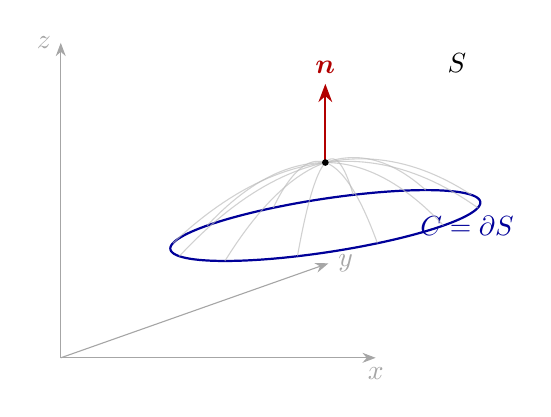
\begin{tikzpicture}[scale=1.0,
  x={(1.0cm,0.0cm)},
  y={(0.85cm,0.30cm)},
  z={(0.0cm,1.0cm)}]

  % axes
  \draw[-{Stealth},gray!70] (0,0,0) -- (4.0,0,0) node[below] {$x$};
  \draw[-{Stealth},gray!70] (0,0,0) -- (0,4.0,0) node[right] {$y$};
  \draw[-{Stealth},gray!70] (0,0,0) -- (0,0,4.0) node[left] {$z$};

  % draw a "cap" surface (schematic) and boundary circle
  % boundary circle in plane z=1.2 with radius 1.5 centered at (2,1.6)
  \coordinate (C0) at (2.0,1.6,1.2);
  \pgfmathsetmacro{\R}{1.5}

  % boundary circle
  \draw[thick,blue!60!black]
    plot[variable=\t,domain=0:360,samples=160]
    ({2.0+\R*cos(\t)},{1.6+\R*sin(\t)},{1.2});
  \node[blue!60!black] at (3.8,1.6,1.2) {$C=\partial S$};

  % surface patch as a dome: z = 1.2 + 0.8*(1 - (r/R)^2), r<=R (schematic grid)
  \foreach \u in {0,30,...,330} {
    \draw[gray!55,opacity=0.65]
      plot[variable=\rr,domain=0:\R,samples=25]
      ({2.0+\rr*cos(\u)},{1.6+\rr*sin(\u)},{1.2+0.8*(1-(\rr/\R)^2)});
  }

  % normal vector at a top point
  \coordinate (Top) at (2.0,1.6,{1.2+0.8});
  \draw[-{Stealth},thick,red!70!black] (Top) -- (2.0,1.6,{1.2+0.8+1.0}) node[above] {$\vect n$};
  \fill (Top) circle (1.2pt);

  \node at (1.8,3.8,2.6) {$S$};

\end{tikzpicture}
\caption{Stokes' theorem relates a line integral around $C=\partial S$ to the flux of $\nabla\times \vect F$ through the surface $S$.}
\label{fig:stokes-geom}
\end{figure}

\begin{exercise}
Let $\vect F=\langle y,-x,0\rangle$ and let $C$ be the circle $x^2+y^2=4$ in the plane $z=3$, oriented counterclockwise when viewed from above.
Use Stokes' theorem to compute $\displaystyle \oint_C \vect F\cdot d\vect r$ by choosing a convenient surface.
\end{exercise}

\begin{exercise}
Use the divergence theorem to compute the outward flux of $\vect F=\langle x^3,y^3,z^3\rangle$ across the boundary of the cube $0\le x,y,z\le 1$.
\end{exercise}

\subsubsection*{Chapter 7 Checklist}
\begin{itemize}
\item Vector fields $\vect F=\langle P,Q\rangle$ (2D) or $\langle P,Q,R\rangle$ (3D) model flow/force.
\item Scalar line integral: $\displaystyle \int_C f\,ds=\int_a^b f(\vect r(t))\|\vect r'(t)\|\,dt$.
\item Work integral: $\displaystyle \int_C \vect F\cdot d\vect r=\int_a^b \vect F(\vect r(t))\cdot \vect r'(t)\,dt$.
\item Fundamental Theorem for Line Integrals: if $\vect F=\nabla f$, then $\int_C \vect F\cdot d\vect r=f(B)-f(A)$.
\item Green's theorem: boundary circulation/flux $\leftrightarrow$ interior double integral.
\item Divergence $\nabla\cdot \vect F=P_x+Q_y+R_z$ and curl $\nabla\times \vect F=\langle R_y-Q_z,\ P_z-R_x,\ Q_x-P_y\rangle$.
\item Stokes: $\displaystyle \oint_{\partial S} \vect F\cdot d\vect r=\iint_S (\nabla\times \vect F)\cdot \vect n\,dS$.
\item Divergence theorem: $\displaystyle \iint_{\partial E}\vect F\cdot \vect n\,dS=\iiint_E (\nabla\cdot \vect F)\,dV$.
\end{itemize}

% =========================
% End of Chapter 7
% =========================

% =========================
% Chapter 8 (no preamble)
% =========================

\section{Chapter 8: Parametric Surfaces and Surface Integrals}

\begin{keyidea}
Curves are 1-dimensional objects, so we integrate along them with $ds$ or $d\vect r$.  
Surfaces are 2-dimensional objects, so we integrate over them with an area element $dS$.

The key geometric fact is: a smooth surface can be \emph{parameterized} by two variables $(u,v)$, and the tiny surface patch area is controlled by the cross product
\[
\bigl\|\vect r_u\times \vect r_v\bigr\|.
\]
That single quantity drives both surface area and surface integrals (scalar and flux).
\end{keyidea}

% -------------------------------------------------
\subsection{Lesson 8.1: Parametric Surfaces}

\subsubsection{Parametrizations and Tangent Planes}

\begin{definition}[Parametric surface]\label{def:param-surface}
A \emph{parametric surface} is a vector-valued function
\[
\vect r(u,v)=\langle x(u,v),\,y(u,v),\,z(u,v)\rangle,
\]
defined on a region $D^\ast\subset \RR^2$ (the \emph{parameter domain}). The image
\[
S=\{\vect r(u,v):(u,v)\in D^\ast\}\subset\RR^3
\]
is the surface.
\end{definition}

\begin{definition}[Tangent vectors and normal]\label{def:tangent-normal}
If $\vect r$ has continuous partial derivatives, then the vectors
\[
\vect r_u=\frac{\partial \vect r}{\partial u},\qquad \vect r_v=\frac{\partial \vect r}{\partial v}
\]
are tangent to the surface (they point along the $u$- and $v$-coordinate curves).  
If $\vect r_u\times \vect r_v\neq \vect 0$, then a normal vector to the surface is
\[
\vect n = \vect r_u\times \vect r_v.
\]
\end{definition}

\begin{proposition}[Tangent plane to a parametric surface]\label{prop:tangent-plane-param}
At a point $\vect r(u_0,v_0)$ with $\vect r_u\times \vect r_v\neq\vect 0$, the tangent plane is the plane through $\vect r(u_0,v_0)$ with normal $\vect n=\vect r_u(u_0,v_0)\times \vect r_v(u_0,v_0)$:
\[
\vect n\cdot\bigl(\langle x,y,z\rangle-\vect r(u_0,v_0)\bigr)=0.
\]
\end{proposition}

\begin{remark}[Plain-language picture]
A surface is locally like a stretched sheet. The vectors $\vect r_u$ and $\vect r_v$ span the local directions you can move while staying on the sheet. Their cross product points perpendicular to the sheet.
\end{remark}

\begin{example}[A plane as a parametric surface]\label{ex:param-plane}
The plane $z=1+x+2y$ can be parameterized by letting $u=x$ and $v=y$:
\[
\vect r(u,v)=\langle u,\ v,\ 1+u+2v\rangle,\qquad (u,v)\in\RR^2.
\]
Then
\[
\vect r_u=\langle 1,0,1\rangle,\qquad \vect r_v=\langle 0,1,2\rangle,
\]
so a normal is
\[
\vect r_u\times\vect r_v=
\begin{vmatrix}
\vect i & \vect j & \vect k\\
1&0&1\\
0&1&2
\end{vmatrix}
=\langle -1,-2,1\rangle.
\]
\end{example}

\begin{figure}[H]
\centering
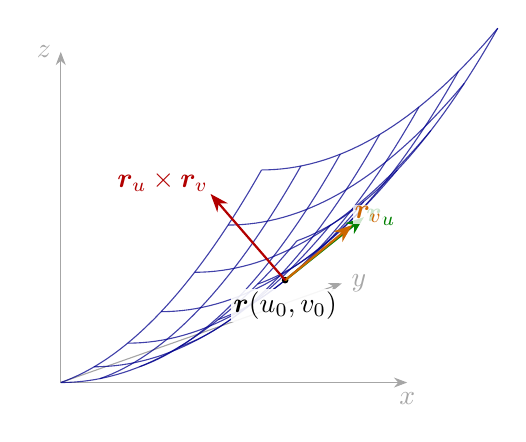
\begin{tikzpicture}[scale=1.0,
  x={(1.0cm,0.0cm)},
  y={(0.85cm,0.30cm)},
  z={(0.0cm,1.0cm)}]

  % --- 1. 变量重命名 (避免使用 \b) ---
  \pgfmathsetmacro{\valu}{2.0} % 原来的 \a
  \pgfmathsetmacro{\valv}{1.0} % 原来的 \b

  % axes
  \draw[-{Stealth},gray!70] (0,0,0) -- (4.4,0,0) node[below] {$x$};
  \draw[-{Stealth},gray!70] (0,0,0) -- (0,4.2,0) node[right] {$y$};
  \draw[-{Stealth},gray!70] (0,0,0) -- (0,0,4.2) node[left] {$z$};

  % surface patch
  \foreach \u in {0,0.5,...,3} {
    \draw[blue!55!black,opacity=0.75]
      plot[variable=\v,domain=0:3,samples=35]
      ({\u},{\v},{0.20*(\u*\u+\v*\v)});
  }
  \foreach \v in {0,0.5,...,3} {
    \draw[blue!55!black,opacity=0.75]
      plot[variable=\u,domain=0:3,samples=35]
      ({\u},{\v},{0.20*(\u*\u+\v*\v)});
  }

  % --- 2. 计算点 P ---
  \pgfmathsetmacro{\zz}{0.20*(\valu*\valu+\valv*\valv)}
  \coordinate (P) at (\valu,\valv,\zz);
  
  \fill (P) circle (1.2pt);
  % 修改位置：改为 below，并加上白色背景 fill=white, opacity=0.8
  \node[below=3pt, fill=white, inner sep=1pt, opacity=0.9, text opacity=1] at (P) {$\vect r(u_0,v_0)$};

  % --- 3. 绘制切向量 ---
  \pgfmathsetmacro{\dxz}{0.40*\valu}
  \pgfmathsetmacro{\dyz}{0.40*\valv}

  % r_u (绿色)
  \draw[-{Stealth},thick,green!50!black]
    (P) -- ({\valu+1.0},{\valv},{\zz+1.0*\dxz})
    % 加上白色背景
    node[right, fill=white, inner sep=0.5pt, opacity=0.8, text opacity=1] {$\vect r_u$};

  % r_v (橙色)
  \draw[-{Stealth},thick,orange!80!black]
    (P) -- ({\valu},{\valv+1.0},{\zz+1.0*\dyz})
    % 加上白色背景，位置微调为 above right
    node[above right, fill=white, inner sep=0.5pt, opacity=0.8, text opacity=1] {$\vect r_v$};

  % --- 4. 法向量 ---
  % normal direction
  \draw[-{Stealth},thick,red!70!black]
    (P) -- ({\valu-0.65},{\valv-0.35},{\zz+1.2})
    % 加上白色背景
    node[above left, fill=white, inner sep=0.5pt, opacity=0.8, text opacity=1] {$\vect r_u\times \vect r_v$};

\end{tikzpicture}
\caption{A surface patch with two tangent directions and a normal direction at a point.}
\label{fig:param-surface}
\end{figure}

\begin{exercise}
Parameterize the cylinder $x^2+y^2=9$ for $0\le z\le 2$ using $(\theta,z)$, and compute $\vect r_\theta\times \vect r_z$.
\end{exercise}

% -------------------------------------------------
\subsection{Lesson 8.2: Surface Area}

\subsubsection{Surface Area of a Parametric Surface}

\begin{theorem}[Surface area formula]\label{thm:surface-area}
Let $S$ be parametrized by $\vect r(u,v)$ on a region $D^\ast$ and assume $\vect r_u\times \vect r_v$ is continuous and nonzero on $D^\ast$. Then the surface area is
\begin{equation}\label{eq:surface-area}
\operatorname{Area}(S)=\iint_{D^\ast}\bigl\|\vect r_u\times \vect r_v\bigr\|\,du\,dv.
\end{equation}
\end{theorem}

\begin{remark}[What $\|\vect r_u\times \vect r_v\|$ is doing]
In the parameter domain, a tiny rectangle has area $du\,dv$. On the surface, it becomes a tiny parallelogram spanned by $\vect r_u\,du$ and $\vect r_v\,dv$, whose area is $\|\vect r_u\times \vect r_v\|\,du\,dv$. Integrating adds them up.
\end{remark}

\subsubsection{Graph Surfaces: $z=g(x,y)$}

\begin{proposition}[Surface area element for a graph]\label{prop:graph-dS}
If $S$ is the graph $z=g(x,y)$ over a region $D$ in the $xy$-plane, and $g_x,g_y$ are continuous on $D$, then
\begin{equation}\label{eq:dS-graph}
dS=\sqrt{1+g_x(x,y)^2+g_y(x,y)^2}\,dA.
\end{equation}
Hence
\[
\operatorname{Area}(S)=\iint_D \sqrt{1+g_x^2+g_y^2}\,dA.
\]
\end{proposition}

\begin{example}[Surface area of a paraboloid patch]\label{ex:paraboloid-area}
Find the area of the surface $z=x^2+y^2$ above the disk $x^2+y^2\le R^2$.

Here $g_x=2x$ and $g_y=2y$, so by \cref{eq:dS-graph},
\[
dS=\sqrt{1+4x^2+4y^2}\,dA=\sqrt{1+4r^2}\,dA
\]
in polar coordinates. Thus
\[
\operatorname{Area}
=\int_{0}^{2\pi}\int_{0}^{R}\sqrt{1+4r^2}\,r\,dr\,d\theta.
\]
Compute the $r$-integral. Let $u=1+4r^2$, so $du=8r\,dr$ and $r\,dr=\frac{1}{8}du$:
\[
\int_0^R r\sqrt{1+4r^2}\,dr
=\frac{1}{8}\int_{1}^{1+4R^2} u^{1/2}\,du
=\frac{1}{8}\cdot \frac{2}{3}\Big[u^{3/2}\Big]_{1}^{1+4R^2}
=\frac{1}{12}\left((1+4R^2)^{3/2}-1\right).
\]
Therefore
\[
\operatorname{Area}
=2\pi\cdot \frac{1}{12}\left((1+4R^2)^{3/2}-1\right)
=\frac{\pi}{6}\left((1+4R^2)^{3/2}-1\right).
\]
\end{example}

\begin{example}[Surface area of a sphere]\label{ex:sphere-area}
Parameterize the sphere of radius $a>0$ by spherical angles:
\[
\vect r(\phi,\theta)=\langle a\sin\phi\cos\theta,\ a\sin\phi\sin\theta,\ a\cos\phi\rangle,
\qquad 0\le \phi\le \pi,\ 0\le\theta\le 2\pi.
\]
Compute partial derivatives:
\[
\vect r_\phi=\langle a\cos\phi\cos\theta,\ a\cos\phi\sin\theta,\ -a\sin\phi\rangle,\qquad
\vect r_\theta=\langle -a\sin\phi\sin\theta,\ a\sin\phi\cos\theta,\ 0\rangle.
\]
A direct computation gives
\[
\bigl\|\vect r_\phi\times \vect r_\theta\bigr\|=a^2\sin\phi.
\]
Therefore, by \cref{eq:surface-area},
\[
\operatorname{Area}(S)
=\int_{0}^{2\pi}\int_{0}^{\pi} a^2\sin\phi\,d\phi\,d\theta
=a^2\left(\int_{0}^{2\pi}d\theta\right)\left(\int_{0}^{\pi}\sin\phi\,d\phi\right)
=a^2(2\pi)(2)=4\pi a^2.
\]
\end{example}

\begin{exercise}
Use \cref{prop:graph-dS} to set up the surface area of $z=xy$ over the rectangle $0\le x\le 1$, $0\le y\le 2$.
(You do not need to evaluate the integral.)
\end{exercise}

% -------------------------------------------------
\subsection{Lesson 8.3: Surface Integrals of Scalar Fields}

\subsubsection{Definition}

\begin{definition}[Surface integral of a scalar function]\label{def:surface-scalar}
Let $S$ be a smooth surface and let $f$ be continuous on $S$. The \emph{surface integral} of $f$ over $S$ is denoted
\[
\iint_S f\,dS.
\]
If $S$ is parametrized by $\vect r(u,v)$ on $D^\ast$, then
\begin{equation}\label{eq:surface-scalar-param}
\iint_S f\,dS
=
\iint_{D^\ast} f(\vect r(u,v))\,\bigl\|\vect r_u\times \vect r_v\bigr\|\,du\,dv.
\end{equation}
\end{definition}

\begin{remark}[Interpretation]
$\iint_S f\,dS$ adds up $f$ weighted by surface area.  
If $f$ is a surface density (mass per unit area), then $\iint_S f\,dS$ is total mass of a thin shell.
\end{remark}

\subsubsection{Graph Case}

\begin{proposition}[Scalar surface integral over a graph]\label{prop:surface-scalar-graph}
If $S$ is $z=g(x,y)$ over a region $D$ in the $xy$-plane, then
\begin{equation}\label{eq:surface-scalar-graph}
\iint_S f\,dS
=
\iint_D f(x,y,g(x,y))\,\sqrt{1+g_x^2+g_y^2}\,dA.
\end{equation}
\end{proposition}

\begin{example}[A clean computation on a plane]\label{ex:scalar-plane}
Let $S$ be the part of the plane $z=1+x+y$ above the unit square $D=\{(x,y):0\le x\le 1,\ 0\le y\le 1\}$, and let $f(x,y,z)=z$.

Here $g(x,y)=1+x+y$, so $g_x=1$ and $g_y=1$. Thus
\[
\sqrt{1+g_x^2+g_y^2}=\sqrt{1+1+1}=\sqrt{3}.
\]
By \cref{eq:surface-scalar-graph},
\[
\iint_S z\,dS
=\iint_D (1+x+y)\sqrt{3}\,dA
=\sqrt{3}\int_{0}^{1}\int_{0}^{1}(1+x+y)\,dy\,dx.
\]
Compute:
\[
\int_{0}^{1}(1+x+y)\,dy=(1+x)\cdot 1+\frac12=\frac32+x,
\qquad
\int_{0}^{1}\left(\frac32+x\right)\,dx=\frac32+\frac12=2.
\]
Therefore
\[
\iint_S z\,dS = 2\sqrt{3}.
\]
\end{example}

\begin{exercise}
Let $S$ be the hemisphere $x^2+y^2+z^2=1$ with $z\ge 0$ and let $f(x,y,z)=z$.
Write $\iint_S f\,dS$ using a spherical parametrization. (You do not need to evaluate.)
\end{exercise}

% -------------------------------------------------
\subsection{Lesson 8.4: Surface Integrals of Vector Fields (Flux)}

\subsubsection{Oriented Surfaces and Flux}

\begin{definition}[Oriented surface]\label{def:oriented-surface}
A smooth surface $S$ is \emph{oriented} if we choose a continuous unit normal vector $\vect n$ at each point of $S$.  
For a closed surface, the standard orientation is \emph{outward}. For a graph $z=g(x,y)$, a common choice is \emph{upward} (positive $z$-component).
\end{definition}

\begin{definition}[Flux integral]\label{def:flux}
Let $\vect F$ be a vector field and let $S$ be an oriented surface with unit normal $\vect n$. The \emph{flux} of $\vect F$ through $S$ is
\begin{equation}\label{eq:flux}
\iint_S \vect F\cdot \vect n\,dS.
\end{equation}
\end{definition}

\begin{remark}[Plain-language meaning]
$\vect F\cdot \vect n$ measures how much the field points through the surface (perpendicular component). Integrating adds up that “through-flow” over the entire surface.
\end{remark}

\subsubsection{Flux Using a Parametrization}

\begin{proposition}[Flux via $\vect r_u\times \vect r_v$]\label{prop:flux-param}
If $S$ is parametrized by $\vect r(u,v)$ on $D^\ast$ and oriented consistently with the normal
\[
\vect n\,dS = \bigl(\vect r_u\times \vect r_v\bigr)\,du\,dv,
\]
then
\begin{equation}\label{eq:flux-param}
\iint_S \vect F\cdot \vect n\,dS
=
\iint_{D^\ast} \vect F(\vect r(u,v))\cdot\bigl(\vect r_u\times \vect r_v\bigr)\,du\,dv.
\end{equation}
If the opposite orientation is required, replace $\vect r_u\times \vect r_v$ by its negative.
\end{proposition}

\subsubsection{Flux Through a Graph Surface}

\begin{proposition}[Flux for a graph $z=g(x,y)$]\label{prop:flux-graph}
Let $S$ be the graph $z=g(x,y)$ over a region $D$ in the $xy$-plane.
A parametrization is $\vect r(x,y)=\langle x,y,g(x,y)\rangle$.
Then
\[
\vect r_x=\langle 1,0,g_x\rangle,\qquad \vect r_y=\langle 0,1,g_y\rangle,
\qquad
\vect r_x\times\vect r_y=\langle -g_x,-g_y,1\rangle.
\]
For the \emph{upward} orientation (positive $z$-component), we have
\begin{equation}\label{eq:flux-graph}
\iint_S \vect F\cdot \vect n\,dS
=
\iint_D \vect F(x,y,g(x,y))\cdot \langle -g_x,-g_y,1\rangle\,dA.
\end{equation}
For the \emph{downward} orientation, use the negative of this vector.
\end{proposition}

\begin{example}[A flux integral that collapses nicely]\label{ex:flux-plane}
Let $\vect F=\langle x,y,z\rangle$, and let $S$ be the part of the plane
\[
z=2-x-y
\]
above the triangle $D=\{(x,y): x\ge 0,\ y\ge 0,\ x+y\le 1\}$, oriented upward.

Here $g(x,y)=2-x-y$, so $g_x=-1$ and $g_y=-1$. By \cref{eq:flux-graph},
\[
\vect n\,dS=\langle -g_x,-g_y,1\rangle\,dA=\langle 1,1,1\rangle\,dA.
\]
Also
\[
\vect F(x,y,g)=\langle x,\ y,\ 2-x-y\rangle,
\quad\Rightarrow\quad
\vect F\cdot \langle 1,1,1\rangle = x+y+(2-x-y)=2.
\]
Therefore the flux is
\[
\iint_S \vect F\cdot \vect n\,dS
=
\iint_D 2\,dA
=2\cdot \operatorname{Area}(D).
\]
The triangle $D$ has legs of length $1$ and $1$, so $\operatorname{Area}(D)=\frac12$. Hence the flux is
\[
\iint_S \vect F\cdot \vect n\,dS = 1.
\]
\end{example}

\begin{exercise}
Let $\vect F=\langle 0,0,z\rangle$ and let $S$ be the graph $z=x^2+y^2$ over the disk $x^2+y^2\le 1$, oriented upward.
Set up $\iint_S \vect F\cdot \vect n\,dS$ using \cref{eq:flux-graph}, and simplify the integrand as much as possible.
\end{exercise}

% -------------------------------------------------
\subsection{Lesson 8.5: Orientation, Boundaries, and Strategy}

\subsubsection{Orientation Conventions}

\begin{remark}[Right-hand rule]
If a surface $S$ has boundary curve $C=\partial S$ and $S$ is oriented by $\vect n$, then the positive orientation of $C$ is given by the right-hand rule: curling the fingers of your right hand in the direction of $C$, your thumb points in the direction of $\vect n$.
\end{remark}

\subsubsection{Choosing the Best Method}

\begin{proposition}[Workflow for surface integrals]\label{prop:surface-workflow}
To compute surface area or a surface integral:
\begin{enumerate}[label=(\arabic*)]
\item Decide whether the surface is best described as a \emph{graph} $z=g(x,y)$ or a \emph{parametric surface} $\vect r(u,v)$.
\item For area or scalar surface integrals, compute the factor $\|\vect r_u\times\vect r_v\|$ (or $\sqrt{1+g_x^2+g_y^2}$).
\item For flux, compute the oriented normal element $\vect n\,dS$:
\[
\vect n\,dS = (\vect r_u\times \vect r_v)\,du\,dv
\quad\text{or}\quad
\vect n\,dS=\langle -g_x,-g_y,1\rangle\,dA
\]
with the correct sign for orientation.
\item Translate the region into clean bounds in the parameter domain (often polar/cylindrical is the cleanest).
\end{enumerate}
\end{proposition}

\begin{figure}[H]
\centering
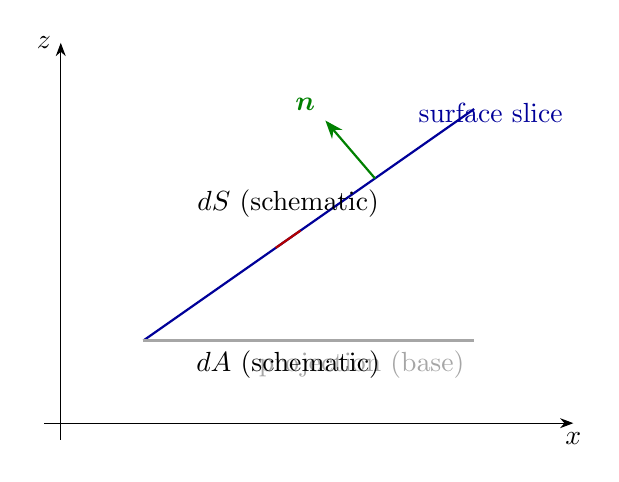
\begin{tikzpicture}[scale=1.05]
  % axes
  \draw[-{Stealth}] (-0.2,0) -- (6.2,0) node[below] {$x$};
  \draw[-{Stealth}] (0,-0.2) -- (0,4.6) node[left] {$z$};

  % slanted line representing surface in a 2D cross-section
  \draw[thick,blue!60!black] (1,1) -- (5,3.8);
  \node[blue!60!black] at (5.2,3.75) {surface slice};

  % base segment (projection)
  \draw[thick,gray!70] (1,1) -- (5,1);
  % 【修改1】将 projection 标签移到最右端，避开左边的 dA
  \node[gray!70, below left] at (5,1) {projection (base)};

  % tiny base dx and corresponding ds
  \coordinate (A) at (2.6,1);
  \coordinate (B) at (2.9,1);
  \draw[thick,gray!70] (A)--(B);
  \node[below] at (2.75,1) {$dA$ (schematic)};

  % corresponding tiny segment on the surface
  \coordinate (As) at (2.6,{1+0.7*(2.6-1)});
  \coordinate (Bs) at (2.9,{1+0.7*(2.9-1)});
  \draw[thick,red!70!black] (As)--(Bs);
  % 【修改2】添加 sloped 让文字倾斜，视觉更整洁
  \node[above, sloped] at (2.75,{1+0.7*(2.75-1)+0.15}) {$dS$ (schematic)};

  % normal arrow (schematic)
  % 【修改3】将法向量的位置从 x=3.3 移到 x=3.8，彻底避开 dS 的文字
  \coordinate (M) at (3.8,{1+0.7*(3.8-1)});
  \draw[-{Stealth},thick,green!50!black] (M) -- ++(-0.6,0.7) node[above left] {$\vect n$};

\end{tikzpicture}
\caption{Schematic idea: $dS$ (surface element) is larger than its projection $dA$ when the surface tilts; the factor $\sqrt{1+g_x^2+g_y^2}$ measures the tilt.}
\label{fig:dS-vs-dA}
\end{figure}

\begin{exercise}
A surface is given parametrically by $\vect r(u,v)=\langle u,\ v,\ uv\rangle$ on $0\le u\le 1$, $0\le v\le 2$.
\begin{enumerate}[label=(\alph*)]
\item Compute $\|\vect r_u\times \vect r_v\|$.
\item Set up the surface area integral.
\item Set up $\iint_S z\,dS$.
\end{enumerate}
\end{exercise}

\subsubsection*{Chapter 8 Checklist}
\begin{itemize}
\item Parametric surface: $\vect r(u,v)$; tangent vectors $\vect r_u,\vect r_v$; normal $\vect r_u\times \vect r_v$.
\item Surface area: $\displaystyle \operatorname{Area}(S)=\iint_{D^\ast}\|\vect r_u\times\vect r_v\|\,du\,dv$.
\item Graph surface $z=g(x,y)$: $\displaystyle dS=\sqrt{1+g_x^2+g_y^2}\,dA$.
\item Scalar surface integral: $\displaystyle \iint_S f\,dS=\iint_{D^\ast} f(\vect r(u,v))\|\vect r_u\times\vect r_v\|\,du\,dv$.
\item Flux integral: $\displaystyle \iint_S \vect F\cdot\vect n\,dS=\iint_{D^\ast}\vect F(\vect r(u,v))\cdot(\vect r_u\times\vect r_v)\,du\,dv$ (orientation matters).
\item For graphs, upward flux uses $\langle -g_x,-g_y,1\rangle\,dA$.
\end{itemize}

% =========================
% End of Chapter 8
% =========================

% =========================
% Chapter 9 (no preamble)
% =========================

\section{Chapter 9: The Big Theorems of Vector Calculus}

\begin{keyidea}
Vector calculus has three “bridge theorems” that convert difficult integrals into easier ones:

\begin{itemize}
\item \textbf{Green's Theorem (2D)}: boundary line integral $\leftrightarrow$ interior double integral.
\item \textbf{Stokes' Theorem (3D)}: boundary circulation $\leftrightarrow$ surface integral of curl.
\item \textbf{Divergence Theorem (3D)}: surface flux $\leftrightarrow$ volume integral of divergence.
\end{itemize}

They all share the same philosophy: \emph{what happens on the boundary is controlled by what happens inside}.
\end{keyidea}

% -------------------------------------------------
\subsection{Lesson 9.1: A Unifying View (Orientation and Boundaries)}

\subsubsection{Orientation in 2D and 3D}

\begin{remark}[Orientation is not optional]
Each theorem requires a consistent orientation:
\begin{itemize}
\item In the plane, \emph{positive orientation} means the boundary curve is traversed counterclockwise.
\item In space, the \emph{right-hand rule} ties the orientation of a boundary curve $\partial S$ to the chosen normal on the surface $S$.
\item For closed surfaces, the standard is \emph{outward} orientation.
\end{itemize}
If you flip the orientation, the integral changes sign.
\end{remark}

\subsubsection{A Quick “Boundary-of-a-Boundary” Principle}

\begin{proposition}[Boundary of a boundary is empty]\label{prop:boundary-boundary}
Informally, $\partial(\partial S)=\varnothing$.
In practice: if you take a surface boundary curve $C=\partial S$, then $C$ has no boundary endpoints because it is a closed loop.
This principle underlies why “curl of a gradient” and “divergence of a curl” vanish.
\end{proposition}

\begin{remark}[What to remember]
The big theorems are “consistent bookkeeping” rules for how derivatives measure interior behavior and integrals measure accumulated boundary behavior.
\end{remark}

% -------------------------------------------------
\subsection{Lesson 9.2: Green's Theorem (Both Forms and Consequences)}

\subsubsection{Statements}

\begin{theorem}[Green's Theorem: circulation form]\label{thm:green9}
Let $C$ be a positively oriented, simple, closed, piecewise-smooth curve in the plane, and let $D$ be the region it encloses.  
If $\vect F=\langle P,Q\rangle$ has continuous partial derivatives on an open set containing $D$, then
\begin{equation}\label{eq:green9-circ}
\oint_C P\,dx+Q\,dy
=
\iint_D \left(\frac{\partial Q}{\partial x}-\frac{\partial P}{\partial y}\right)\,dA.
\end{equation}
\end{theorem}

\begin{theorem}[Green's Theorem: flux form]\label{thm:green9-flux}
Under the same hypotheses,
\begin{equation}\label{eq:green9-flux}
\oint_C \vect F\cdot \vect n\,ds
=
\oint_C P\,dy - Q\,dx
=
\iint_D \left(\frac{\partial P}{\partial x}+\frac{\partial Q}{\partial y}\right)\,dA.
\end{equation}
\end{theorem}

\begin{remark}[Two key operators in 2D]
\[
\text{2D curl (scalar)}:\quad \frac{\partial Q}{\partial x}-\frac{\partial P}{\partial y},
\qquad
\text{2D divergence}:\quad \frac{\partial P}{\partial x}+\frac{\partial Q}{\partial y}.
\]
Green's theorem converts boundary circulation/flux into interior integrals of these quantities.
\end{remark}

\subsubsection{Consequences}

\begin{corollary}[Area formula]\label{cor:area-green9}
If $C=\partial D$ is positively oriented, then
\begin{equation}\label{eq:area-green9}
\operatorname{Area}(D)=\frac12\oint_C (x\,dy-y\,dx).
\end{equation}
\end{corollary}

\begin{proof}
Take $P=-y/2$ and $Q=x/2$. Then $Q_x-P_y=1$ and apply \cref{eq:green9-circ}.
\end{proof}

\begin{corollary}[Circulation is zero for conservative fields]\label{cor:green-conservative}
If $\vect F=\nabla f$ on a region containing $D$, then
\[
\oint_C \vect F\cdot d\vect r=0.
\]
\end{corollary}

\begin{proof}
If $\vect F=\langle P,Q\rangle=\nabla f$, then $P=f_x$ and $Q=f_y$, so $Q_x-P_y=f_{yx}-f_{xy}=0$ (Clairaut). Apply \cref{eq:green9-circ}.
\end{proof}

\subsubsection{Worked Example}

\begin{example}[Use Green instead of parametrizing]\label{ex:green9-example}
Compute $\displaystyle \oint_C (x^2-y^2)\,dx + 2xy\,dy$ where $C$ is the circle $x^2+y^2=4$ oriented counterclockwise.

Here $P=x^2-y^2$ and $Q=2xy$. Then
\[
\frac{\partial Q}{\partial x}-\frac{\partial P}{\partial y}=2y-(-2y)=4y.
\]
So by \cref{eq:green9-circ},
\[
\oint_C P\,dx+Q\,dy=\iint_D 4y\,dA,
\]
where $D$ is the disk $x^2+y^2\le 4$. The integrand $4y$ is odd in $y$ and the disk is symmetric about the $x$-axis, hence
\[
\iint_D 4y\,dA=0.
\]
Therefore the line integral is $0$.
\end{example}

\begin{exercise}
Let $C$ be the positively oriented boundary of the region between the circles $x^2+y^2=1$ and $x^2+y^2=4$.
Use Green's theorem to compute $\displaystyle \oint_C (-y)\,dx + x\,dy$.
\end{exercise}

% -------------------------------------------------
\subsection{Lesson 9.3: Stokes' Theorem (Circulation $\leftrightarrow$ Curl Flux)}

\subsubsection{Statement}

\begin{theorem}[Stokes' Theorem]\label{thm:stokes9}
Let $S$ be an oriented, piecewise-smooth surface with boundary curve $C=\partial S$.
Let $\vect n$ be the unit normal to $S$ consistent with the orientation of $C$ (right-hand rule).
If $\vect F$ has continuous partial derivatives on an open region containing $S$, then
\begin{equation}\label{eq:stokes9}
\oint_{C} \vect F\cdot d\vect r
=
\iint_{S} (\nabla\times \vect F)\cdot \vect n\,dS.
\end{equation}
\end{theorem}

\begin{remark}[Core strategy]
When you see a circulation integral $\oint_C \vect F\cdot d\vect r$, ask:
\begin{itemize}
\item Can I choose a surface $S$ with boundary $C$ that makes the surface integral easy?
\item Often the easiest $S$ is a flat disk, a plane piece, or any simple surface with the same boundary.
\end{itemize}
Stokes' theorem guarantees you can swap surfaces as long as the boundary and orientation match.
\end{remark}

\subsubsection{Independence of Surface (Same Boundary)}

\begin{proposition}[Surface choice principle]\label{prop:surface-choice}
If $S_1$ and $S_2$ are two oriented surfaces with the same boundary curve $C$ (and consistent orientation), then
\[
\iint_{S_1} (\nabla\times \vect F)\cdot \vect n\,dS
=
\iint_{S_2} (\nabla\times \vect F)\cdot \vect n\,dS,
\]
provided $\vect F$ is $C^1$ on a region containing both surfaces.
\end{proposition}

\begin{remark}[Why this is true (conceptual)]
Glue $S_1$ and $S_2$ together to form a closed surface (with opposite orientations on $C$ canceling). Then apply the divergence theorem to $\nabla\times \vect F$ and use $\nabla\cdot(\nabla\times \vect F)=0$.
\end{remark}

\subsubsection{Worked Example}

\begin{example}[Circle in a plane: use a disk]\label{ex:stokes9-circle}
Let $\vect F=\langle -y,\ x,\ z\rangle$ and let $C$ be the circle $x^2+y^2=1$ in the plane $z=0$, oriented counterclockwise as viewed from $+z$.
Choose $S$ to be the unit disk in $z=0$ with upward unit normal $\vect n=\langle 0,0,1\rangle$.

Compute curl:
\begin{align*}
\nabla\times \vect F
&= \left\langle R_y-Q_z,\ P_z-R_x,\ Q_x-P_y \right\rangle \\
&= \left\langle
\frac{\partial}{\partial y}(z)-\frac{\partial}{\partial z}(x),\
\frac{\partial}{\partial z}(-y)-\frac{\partial}{\partial x}(z),\
\frac{\partial}{\partial x}(x)-\frac{\partial}{\partial y}(-y)
\right\rangle \\
&= \langle 0-0,\ 0-0,\ 1-(-1)\rangle \\
&= \langle 0,0,2\rangle.
\end{align*}
Then
\[
\iint_S (\nabla\times \vect F)\cdot \vect n\,dS
=
\iint_S 2\,dS
=
2\cdot \pi
=
2\pi.
\]
So by Stokes,
\[
\oint_C \vect F\cdot d\vect r=2\pi.
\]
\end{example}

\begin{exercise}
Let $C$ be the curve of intersection of the plane $z=2$ with the cylinder $x^2+y^2=9$, oriented counterclockwise as viewed from above.
Use Stokes' theorem to compute $\displaystyle \oint_C \langle -y,x,0\rangle\cdot d\vect r$.
\end{exercise}

% -------------------------------------------------
\subsection{Lesson 9.4: Divergence Theorem (Flux $\leftrightarrow$ Divergence Volume Integral)}

\subsubsection{Statement}

\begin{theorem}[Divergence Theorem]\label{thm:div9}
Let $E$ be a solid region in $\RR^3$ with closed, piecewise-smooth boundary surface $S=\partial E$ oriented outward.
If $\vect F$ has continuous partial derivatives on an open region containing $E$, then
\begin{equation}\label{eq:div9}
\iint_{S} \vect F\cdot \vect n\,dS
=
\iiint_{E} (\nabla\cdot \vect F)\,dV.
\end{equation}
\end{theorem}

\begin{remark}[When it is most useful]
If the surface $S$ is complicated but the volume $E$ is simple (e.g., a ball or box), the divergence theorem often turns a hard surface integral into an easy triple integral.
\end{remark}

\subsubsection{Worked Example}

\begin{example}[Flux through a sphere without parametrizing]\label{ex:div9-sphere}
Let $\vect F=\langle x^2, y^2, z^2\rangle$ and let $S$ be the sphere $x^2+y^2+z^2=a^2$ oriented outward.
Then
\[
\nabla\cdot \vect F = 2x+2y+2z.
\]
Let $E$ be the ball $x^2+y^2+z^2\le a^2$. By symmetry,
\[
\iiint_E x\,dV=\iiint_E y\,dV=\iiint_E z\,dV=0
\]
because the ball is symmetric under sign changes in each coordinate. Hence
\[
\iiint_E (2x+2y+2z)\,dV=0.
\]
Therefore, by \cref{eq:div9},
\[
\iint_S \vect F\cdot \vect n\,dS=0.
\]
\end{example}

\begin{example}[Flux through a cube]\label{ex:div9-cube}
Compute the outward flux of $\vect F=\langle x^3,y^3,z^3\rangle$ across the boundary of the cube $0\le x,y,z\le 1$.

We have
\[
\nabla\cdot \vect F = 3x^2+3y^2+3z^2.
\]
Thus, by \cref{eq:div9},
\[
\iint_{\partial E}\vect F\cdot \vect n\,dS
=
\iiint_{E} (3x^2+3y^2+3z^2)\,dV
=
3\iiint_E x^2\,dV + 3\iiint_E y^2\,dV + 3\iiint_E z^2\,dV.
\]
By symmetry of the cube,
\[
\iiint_E x^2\,dV=\iiint_E y^2\,dV=\iiint_E z^2\,dV
=
\left(\int_0^1 x^2\,dx\right)\left(\int_0^1 dy\right)\left(\int_0^1 dz\right)
=\frac13.
\]
Therefore
\[
\iint_{\partial E}\vect F\cdot \vect n\,dS
=
3\left(\frac13+\frac13+\frac13\right)=3.
\]
\end{example}

\begin{exercise}
Let $\vect F=\langle x,y,z\rangle$ and let $S$ be the boundary of the region between the spheres $\rho=1$ and $\rho=2$ (an “outer shell”), oriented outward.
Use the divergence theorem to compute $\iint_S \vect F\cdot \vect n\,dS$.
\end{exercise}

% -------------------------------------------------
\subsection{Lesson 9.5: Putting It All Together (Recognizing the Right Theorem)}

\subsubsection{Decision Guide}

\begin{proposition}[Which theorem should you try first?]\label{prop:decision-guide}
\begin{enumerate}[label=(\arabic*)]
\item If you have a \emph{line integral around a closed curve} in the plane: try \textbf{Green's theorem}.
\item If you have a \emph{line integral around a closed space curve} and you can find a surface spanning it: try \textbf{Stokes' theorem}.
\item If you have a \emph{flux integral across a closed surface}: try the \textbf{Divergence theorem}.
\end{enumerate}
\end{proposition}

\begin{remark}[Common simplifications]
\begin{itemize}
\item Symmetry can zero out integrals immediately (odd integrands over symmetric regions).
\item For Stokes, choose the easiest spanning surface (often a flat disk).
\item For Divergence, avoid parametrizing complicated surfaces—integrate divergence over a simple volume instead.
\end{itemize}
\end{remark}

\subsubsection{A Compact “Unified” Diagram}

\begin{figure}[H]
\centering
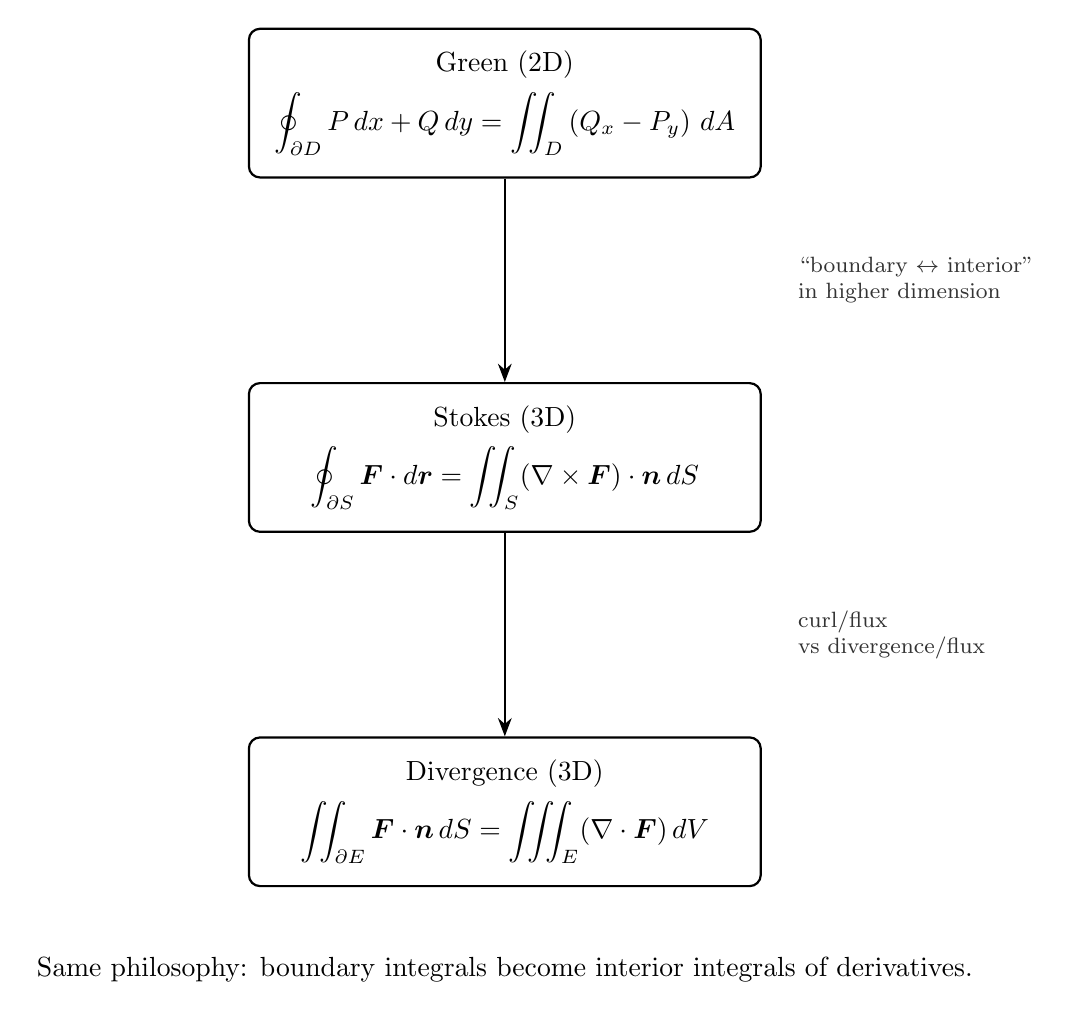
\begin{tikzpicture}[scale=1.0]
  % 定义统一的盒子样式，方便调整
  \tikzset{
    mybox/.style={
      draw, rounded corners, thick, align=center,
      minimum width=6.5cm, minimum height=1.6cm, % 稍微加大高度
      inner sep=8pt
    }
  }

  % 1. 调整坐标：拉大垂直间距 (4.5 -> 0 -> -4.5)
  \node[mybox] (green) at (0,4.5)
    {Green (2D)\\[4pt]
     $\displaystyle \oint_{\partial D} P\,dx+Q\,dy=\iint_D\left(Q_x-P_y\right)\,dA$};

  \node[mybox] (stokes) at (0,0)
    {Stokes (3D)\\[4pt]
     $\displaystyle \oint_{\partial S}\vect F\cdot d\vect r=\iint_S (\nabla\times\vect F)\cdot \vect n\,dS$};

  \node[mybox] (div) at (0,-4.5)
    {Divergence (3D)\\[4pt]
     $\displaystyle \iint_{\partial E}\vect F\cdot \vect n\,dS=\iiint_E (\nabla\cdot\vect F)\,dV$};

  % 2. 绘制箭头
  \draw[-{Stealth},thick] (green) -- (stokes);
  \draw[-{Stealth},thick] (stokes) -- (div);

  % 3. 绘制说明文字 (移到右侧)
  % 盒子的一半宽度约为 3.25cm，我们将文字放在 x=3.6 处，完全避开盒子
  \node[right, align=left, font=\footnotesize, color=gray!40!black] at (3.6, 2.25) 
    {“boundary $\leftrightarrow$ interior”\\ in higher dimension};

  \node[right, align=left, font=\footnotesize, color=gray!40!black] at (3.6, -2.25) 
    {curl/flux\\ vs divergence/flux};

  % 底部总结
  \node[align=center] at (0,-6.5)
    {Same philosophy: boundary integrals become interior integrals of derivatives.};
\end{tikzpicture}
\caption{A high-level map of the three major theorems.}
\label{fig:big-theorems-map}
\end{figure}

\subsubsection{Final Practice Problems}

\begin{exercise}
Let $C$ be the positively oriented boundary of the region $D=\{(x,y):0\le x\le 1,\ 0\le y\le x\}$.
Compute $\displaystyle \oint_C (y^2)\,dx + (x^2)\,dy$ using Green's theorem.
\end{exercise}

\begin{exercise}
Let $S$ be the portion of the plane $x+2y+3z=6$ in the first octant, oriented with upward-pointing normal (positive $z$-component).
Use Stokes' theorem to compute $\displaystyle \oint_{\partial S} \langle y,-x,0\rangle\cdot d\vect r$.
(Hint: choose a convenient spanning surface with the same boundary.)
\end{exercise}

\begin{exercise}
Let $S$ be the boundary of the region $E=\{(x,y,z):x^2+y^2+z^2\le 9\}$ oriented outward.
Compute $\displaystyle \iint_S \langle x,0,0\rangle\cdot \vect n\,dS$ using the divergence theorem.
\end{exercise}

\subsubsection*{Chapter 9 Checklist}
\begin{itemize}
\item Green's theorem (2D): $\displaystyle \oint_{\partial D} P\,dx+Q\,dy=\iint_D (Q_x-P_y)\,dA$ and flux form $\displaystyle \oint_{\partial D} \vect F\cdot \vect n\,ds=\iint_D (P_x+Q_y)\,dA$.
\item Stokes' theorem (3D): $\displaystyle \oint_{\partial S}\vect F\cdot d\vect r=\iint_S (\nabla\times\vect F)\cdot \vect n\,dS$.
\item Divergence theorem (3D): $\displaystyle \iint_{\partial E}\vect F\cdot \vect n\,dS=\iiint_E (\nabla\cdot\vect F)\,dV$.
\item Orientation matters: counterclockwise in the plane, right-hand rule in space, outward for closed surfaces.
\item Strategy: choose the theorem that converts your integral into the simplest region/surface/volume integral available.
\end{itemize}

% =========================
% End of Chapter 9
% =========================

\end{document}